\documentclass{article}

\usepackage{arxiv}

\usepackage{todonotes}
\usepackage[utf8]{inputenc} % allow utf-8 input
\usepackage[T1]{fontenc}    % use 8-bit T1 fonts
\usepackage{hyperref}       % hyperlinks
\usepackage{url}            % simple URL typesetting
\usepackage{booktabs}       % professional-quality tables
\usepackage{amsfonts,amssymb,amsthm}       % blackboard math symbols
\usepackage{nicefrac}       % compact symbols for 1/2, etc.
\usepackage{microtype}      % microtypography
\usepackage{lipsum}
\usepackage{amsmath}
\usepackage{amssymb}
\usepackage{graphicx} % inclusion des figures
\usepackage{braket}
\usepackage{listings}
\usepackage{pgf, tikz}
\usepackage[sorting=none]{biblatex}
\usepackage{pgfplots}
\usepackage{pgfplotstable}
\usetikzlibrary{arrows, automata}
\usetikzlibrary{arrows,shapes}
\pgfplotsset{compat=1.17} 
\usepackage{qcircuit}
\usepackage{caption}
\usepackage{subcaption}

\addbibresource{references.bib}

\newenvironment{changemargin}[2]{%
\begin{list}{}{%
\setlength{\topsep}{0pt}%
\setlength{\leftmargin}{#1}%
\setlength{\rightmargin}{#2}%
\setlength{\listparindent}{\parindent}%
\setlength{\itemindent}{\parindent}%
\setlength{\parsep}{\parskip}%
}%
\item[]}{\end{list}}

\title{Computing PageRank using Quantum Graph Fourier Transform}
\newcommand\advisor{\thanks{Advisor}}

\author{
  Théodore Chapuis-Chkaiban\\
  Department of Computer Science\\
  CentraleSupelec - Paris-Saclay University\\
  3 Rue Joliot-Curie, 91190, Gif-Sur-Yvette, FRANCE\\ 
  \texttt{theodore.chapuis-chkaiban@student-cs.fr}
  %% examples of more authors
\and
 Zeno Toffano \\
  Laboratoire des Signaux et Systèmes (L2S-UMR8506)\\
  CentraleSupelec - Paris-Saclay University\\
  3 Rue Joliot-Curie, 91190, Gif-Sur-Yvette, FRANCE\\
  \texttt{zeno.toffano@centralesupelec.fr}
  \and
  Benoit Valiron \\
  Department of Computer Science\\
  CentraleSupelec - Paris-Saclay University\\
  3 Rue Joliot-Curie, 91190, Gif-Sur-Yvette, FRANCE\\
  \texttt{benoit.valiron@centralesupelec.fr} 
}

\date{\today}

\newtheorem{lem}{Lemma}[section]
\newtheorem{prop}{Proposition}[section]
\newtheorem{propriete}{Property}[section]
\newtheorem{cor}{Corollary}[section]
\newtheorem{definition}{Definition}[section]
\newtheorem{theo}{Theorem}[section]
\newtheorem{definition-theo}{Definition-Theorem}[section]


\begin{document}

\maketitle
 
\begin{abstract}
In this paper, we provide a new computation method of the PageRank algorithm designed by Google relying on the Spectral Graph Theory principles. Supposing one can build an efficient enough QRAM, we achieve PageRank classification at least quadratically faster than on a classical computer, at most exponentially faster for matrices with nodes heavily connected. Besides, our method is fully parallelizable on classical and quantum computers. Finally, our generalized Pagerank allows to access more information on the input Web Graph while preserving the original structure of the graph.
\end{abstract}


% keywords can be removed
\keywords{Quantum Computing \and PageRank \and Fourier Transform \and Spectral Graph Theory}


\section{Introduction}

\todo[inline]{TODO INLINE}

\paragraph{Google PageRank:}
The Google\todo{TODO MARGE} PageRank algorithm was introduced by Sergey Brin and Lawrence Page through their paper entitled "The anatomy of a large-scale hypertextual Web search engine" \cite{brin_page_1998}. This algorithm shaped the Web and even though the PageRank algorithm has been integrated into a larger pipeline to derive web Rankings, it remains a major component of Google's search engine that largely contributed to its fame.\\
The PageRank aims at ranking the nodes of any directed graph by order of importance. We will develop this notion of importance later throughout this paper, but it's worth noting that Google's PageRank derives a nodes ranking based on a very specific conception of importance. \\
Nowadays, one has derived several applications where the PageRank algorithm can be found useful - for instance in any social network, this algorithm can be used to rank the most influential users or content. We have also been able to find use cases in various fields like sports, literature, neuroscience, toxic waste management, debugging and road traffic prediction (see \cite{cornell_pagerank} for more details). David F. Gleich has studied extensively the various applications of the PageRank algorithm in \cite{gleich_2015}.

\paragraph{Computational complexity of the PageRank:} The Google PageRank computational complexity has been studied extensively over the last few years. Since the algorithm relies on the Perron-Frobenius theorem which derives an approximation of the final PageRank vector, one has to precise the maximum error on the prediction for the algorithm.\\
Since nowadays, the computations of the PageRank on the Web Graph involve several billion of web pages, one had to find a parallel implementation of the PageRank algorithm. One remarkable result regarding PageRank parallelization can be found in \cite{sarma_molla_pandurangan_upfal_2013} - however, this result assumes that each node of the graph can perform computations which is not the case in our general setting.\\
In a unparallel setting, the PageRank of a n-nodes graph can be computed in $\mathcal{O}(n^2)$ operations (it amounts to compute the eigenspace associated with the 1 eigenvalue). When it comes to approximating the PageRank, the error on the real value of the Perron vector seems to be lower than $\alpha^k$ after k iterations of the algorithm (involving an $n\times n$ matrix-vector multiplication and a vector-vector addition), where $\alpha$ is a constant between 0.1 and 0.99 used as an initial parameter for the PageRank algorithm.\\


\paragraph{Evolution of Quantum Computing:}
Quantum computing is an exciting field at the crossroads of mathematics, physics and computer science. Over the past two decades, the rise of quantum computing has been considerable and has resulted in several scientific achievements. In 2019, Google claimed to have achieved quantum supremacy by stabilizing a computer of more than 50 Qbits \cite{google2019}: this technical achievement is the result of several decades of research in the field of theoretical physics, but also a mature understanding of technologies that, until very recently, were relegated to the stage of futuristic fads, without much of a future.\\

\paragraph{Spectral Graph Theory:}
Our approach uses Spectral Graph Theory, a recent mathematical theory, to build a consistent algorithm to perform PageRank. Spectral Graph Theory unveils general graph properties thanks to the spectral study of the Graph Laplacian \cite{ricaud2019}. This method allows us to define a Fourier Transform on a directed graph, which will be useful for the our study.\\

\paragraph{Results:}
This paper defines a new framework to solve an adapted version of the PageRank (section \ref{sec:SGTapplicationToPR}). This method relies on Spectral Graph Theory introduced in \ref{sec:SGTIntro}, and allows producing newer and finer rankings thanks to the study of the eigenspaces of the transition matrix of the input Graph. Indeed, we show that our adapted version of the PageRank allows us to refine the ranking obtained by the original PageRank, detecting strongly connected components of the input web pages, and respecting the original structure of the input graph.   \\

Next, we aim at introducing the spectral Graph theory framework to Quantum Computing by deriving a Quantum Circuit enabling the study and the production of signals on graphs. Our work relies on Quantum Signal Processing first introduced by \cite{eldar_oppenheim_2002}, and since then an active study field of Quantum Computing. Some advances in the field include the pioneering works from \cite{Low_2019} on Qubitization, and, more recently, the very comprehensive study performed by Andràs Gilyén, Yuan Su $\&$ Cie \cite{gilyén_su_low_wiebe_2019} on which we will rely to properly define a Quantum Spectral Graph Theory Framework. We show that, providing one has access to an efficient Quantum data structure, one can either perform advanced graph signal filtering or produce complex signals based on inverse Graph Fourier Transform using a number of Quantum gates that scales linearly with the degree of a polynomial approximation of the filter. We then present several Spectral Graph Theory based use case for our algorithm and notably present how our generalized PageRank method can be efficiently implemented thanks to this Quantum Algorithm. As far as we know, this parallel between Spectral Graph Theory and Quantum Signal Processing have not been performed yet and our pioneering work, extending the Quantum Signal Filtering framework to the study and production of complex graphs signals, paves the way for an exciting range of applications in Graph Signal Processing.

Finally, our last contribution remains in defining one of the very first Quantum Circuit based PageRank computing algorithm that can be seen as a gate based equivalent of the Adiabatic version of \cite{garnerone_zanardi_lidar_2012}. However, our version achieves a better theoretical complexity in the final state preparation and relies on the well known and heavily studied Quantum Algorithm for Linear Systems of Equations.
As far as we know, this theoretical logarithmic complexity has never been reached in the scientific literature for the PageRank algorithm, the previous best result was obtained by \cite{garnerone_zanardi_lidar_2012}, featuring a $\mathcal{O}(polylog(n))$ experimental complexity. \\


\paragraph{Structure of this paper:}
We have divided this article into 3 parts:
\begin{enumerate}
    \item Introduction to spectral graph theory, application to the web classification problem.
    \item Quantum translation of the problem.
    \item Results.
\end{enumerate}

\newpage

\tableofcontents

\newpage


\section{Preliminary notions and previous results}
\label{sec:previousResults}

\subsection{General context and applications.}
The Google PageRank algorithm was introduced by Sergey Brin and Lawrence Page through their paper entitled "The anatomy of a large-scale hypertextual Web search engine" \cite{brin_page_1998}. The PageRank algorithm aims at ranking the nodes of any directed graph by order of importance, hence its natural and original application to rank the web pages according to their influence on the network.

More precisely, we are given a graph G = (V, E) whose vertices correspond to Web Pages and $e_{i \rightarrow j} = 1$ iff webpage i has a link pointing to webpage j. G is then an directed graph, embodying the relations between the web pages. The PageRank algorithm outputs a importance function \emph{I}, $I:V \rightarrow \mathbb{R}$, that establishes a ranking of the WebPages by order of importance.

Nowadays, one has derived several applications where the PageRank algorithm can be found useful - for instance in any social network, this algorithm can be used to rank the most influential users or content. We have also been able \cite{cornell_pagerank} to find use cases in various fields like sports (rank the best athletes of a specific sport), literature (rank the most original authors of a given period), neuroscience (neuroscientists identified parts of the brain that changed during the ageing process), toxic waste management (remove nuclear waste and toxic chemicals from infected water), debugging (quantify the contribution of different code parts in an anomalous situation) and road traffic prediction (predict traffic flows). David F. Gleich has studied extensively the various applications of the PageRank algorithm in \cite{gleich_2015}. Instead of representing web pages, the nodes of the network may then represent authors, neurons, sportsmen or even roads - still the method to derive a ranking of these nodes is the same. 

Besides, the original PageRank algorithm has paved the way for several directly related generalizations such as the Total Rank \cite{boldi_2005} or the Heat Kernels and Matrix exponential based ranks \cite{yang_king_lyu_2007}: we will study the relation of these generalizations to our contributions in \ref{subsec:main_consequences} - we will show that our PageRank generalization actually includes these two generalizations as special cases.

Another well-known variant of the PageRank is the personalized PageRank \cite{haveliwala_2003, langville_meyer_2004, gleich_2015}, heavily used in social networks \cite{gleich_2015}. This approach is closely related to the PageRank, however it has several peculiarities that will be detailed in \ref{subsec:preferential_pagerank}. Several authors like \cite{gleich_2015} regard the personalized PageRank as a generalization of the original PageRank, and thus uses the term \textit{PageRank} to designate both methods. 

It is worth noting that, while PageRank is a very popular algorithm as it is used by Google as a part of its search engine, there exists other webpages ranking algorithms - such as HITS (Hyperlink-Induced Topic Search) \cite{kleinberg_hubs, kleinberg_1999} algorithm. However, this algorithm is not adapted to large scale search engines as it needs to recompute the ranking for every query to the database, which is hardly scalable to the actual size of the Web, even tough the query filters a great part of the webpages to rank - in comparison, the PageRank only needs to be computed while indexing the web pages, which can be performed independently from the query process.\\
HITS takes as input the web graph and outputs two different rankings : a hub ranking and an authoritative ranking. This distinction highlights the fact that some webpages are specialised in redirecting to other webpages (such as \textit{google} or \textit{yahoo}), others concentrate most of the traffic, being a highly authoritative entity (such as \textit{netflix} when the query is \textit{video streaming}). Even if this distinction is interesting as it helps understanding why the web pages have high ranking scores, it introduces a query dependency which is not suitable for global, non web search oriented, applications.


\subsection{Mathematical statement of the problem.}

\paragraph{Inputs:} We are given a directed finite weighted graph $\mathcal{G} = (V, E, W(E))$, where
$W(E) : V \times V \rightarrow \mathbb{R}^{+}$ is a map such that $\forall (i,j) \in V\times V, \left\{ \begin{array}{cc}
    W(i,j)>0 & \mbox{ if } (i,j) \in E  \\
    W(i,j)=0 & \mbox{ otherwise}
\end{array} \right.$.
We will only consider finite graphs in this paper, ie $|V|<\infty$.\\
Throughout this paper, to enhance the clarity, one will use the simpler terms \textit{directed graphs} or \textit{graphs} in place of \textit{directed finite weighted graph}, the finite and weighted properties being assumed and implicit if not precised otherwise. Similarly, the terms \textit{weighted adjacency matrix} and \textit{adjacency matrix} will be used indistinctively.

While the original PageRank can apply to any type of graph, we derived our results by using the algorithm on scale-free networks. The scale free network degree distribution follows a power law asymptotically, ie the proportion P(k) of nodes having k outgoing edges is :
\begin{equation*}
    P(k) \simeq k^{-\gamma}
\end{equation*}
Where $2 \leq \gamma \leq 3$, as it seems to lead to models better highlighting human interaction \cite{choromański_matuszak_mie}. 

These scale-free networks are generated using the Barabási–Albert model. In fact, this model produce random scale-free networks using a preferential attachment mechanism - which aims to simulate naturals and human-based systems such as the Internet or Social Networks \cite{barabási_albert_1999, albert_barabási_2002}. These networks incorporate a growth mechanism to simulate the growth of a network over time. Then, the preferential attachment mechanism states that the more a node is connected, the more it is likely to receive new links. 

The Barabási–Albert networks are then generated iteratively, starting from a basis of $m_0$ nodes and adding one node at a time. Each new node is connected to $m \leq m_0$ existing nodes with the probability that it is connected to a given node i being : 
\begin{equation*}
    p_i = \frac{k_i}{\sum_{exist \ nodes j} k_j}
\end{equation*}
$k_i$ being the degree of the node i and the sum being held on all the pre-existing nodes.\\

Besides, we have chosen to produce results using also the Erdős–Rényi model to generate another class of random graphs \cite{erdos}. In fact, these category of graphs does not belong to the class of scale free networks, but rather generates random graphs with a given number of edges and nodes. The results obtained on these graphs will be more general and does not solely apply to scale-free networks.

\paragraph{Result:} An importance vector \emph{I}, $I:V \rightarrow \mathbb{R}$, that establishes a ranking of the nodes by order of "importance". In this definition of the importance vector, one can easily see that the notion of "importance" is not well defined - we will precise this notion in the following subsection.\\

\subsection{Google matrix and Google importance vector.}

\subsubsection{Theoretical prerequisites}
\label{subsubsec:Theo_prepreq}
The PageRank algorithm heavily relies on Random Walks, more specifically on Markov Chains - it uses the Perron Frobenius theorem to compute the importance vector. In this first section, we precise these definitions and theorems that form the very basis of the PageRank theory ; what is more, we define some notations and parallels that will be used throughout this article.

A central notion behind the PageRank algorithm is the one of Markov Chain. Informally, given a directed weighted graph $\mathcal{G} = (V,E, W(E))$ a markov chain can be seen as the successive positions of a random walker on the nodes V, knowing that the random walker can jump from the node $i$ to the node $j$ of $\mathcal{G}$ with the probability $p_{ij} = \frac{W(i,j)}{\sum_{k\in V} W(i,k)} \in [0,1]$. Formally, a Markov chain is defined as : 

\begin{definition}[Markov chain \cite{grinstead_snell_2006}]

Given a set of \textit{states} (which can be seen as nodes of a directed graph), $S=\{s_1, s_2, ..., s_r\}$, a markov chain is a process that starts from one of these states and moves successively from one state to another. Each move is called a \textit{step}. If the chain is currently in state $s_i$, then it moves to state $s_j$ at the next step with a probability $p_{ij}$ (which can be seen as the weight of the edge starting from i, and going into j) - moreover, the probability $p_{ij}$ does not depend upon which states the chain was in before the current state. 

Another way to understand it : a markov chain is a random walk (a family of random processes) on a directed positively weighted and simple (one edge per couple of nodes) graph (with loops), where the weight of each arc stands for the transition probability between the nodes.

\end{definition}

We have then a direct correspondence between the set of states of a Markov chain with its associated transition probabilities and the directed weighted graph $\mathcal{G}=(V, E, W(E))$ where V is exactly the set of states of the Markov chain and $\forall \ (i,j) \in E, p_{ij} = \frac{W_{ij}}{\sum_{k\in V} W_{ik}}$.
Trivially, if $i \in V$ is a node of $\mathcal{G}$, so that $\exists j \in V, (i,j) \in E$, then $\sum_{j \in V} p_{i,j} = 1$.

We will also identify the set of transition probabilities with the weighted adjacency matrix of the directed graph associated with the Markov Chain - which we will call the \textit{transition matrix} of the markov chain. \\
Thus, to simplify the notations, and without restricting our study, we will assume that all the directed weighted graphs $\mathcal{G}=(V, E, W(E))$ introduced in this paper are normalized. Ie, $\forall i \in V$, if $\exists j \in V, \mbox{ so that: } (i,j)\in E$, then $\sum_{j \in V} W(i,j) = 1$. Hence, given a graph $\mathcal{G}$ one will now use indifferently the term \textit{transition matrix} to designate the \textit{adjacency weighted matrix} of $\mathcal{G}$ - this convention simplifies greatly the notations introduced in this paper.

An important notion associated with \textit{transition matrices} is \textit{left-stochasticity}:

\begin{definition}[Left-stochastic matrix]

Let M be a matrix, M is left-stochastic if its line coefficients sum to one, ie:

\begin{equation}
    M e^T = e^T
\end{equation}

Where $e = (1, \hdots, 1)$, the row vector whose coefficients are all equal to one.

\end{definition}

Besides, let's define notion of dangling nodes which is fundamental to the PageRank Theory:

\begin{definition}[Dangling Nodes \cite{langville_meyer_2004}]\label{def:dangling}
Let $\mathcal{G}=(V,E)$ be a directed graph. $x \in V$ is called a dangling node if it has no outgoing edges.
\end{definition}

The \textit{transition matrix} of a Markov Chain on a graph that doesn't have any \textit{dangling nodes} (ie nodes that has no outgoing edges) is \textit{left stochastic}. If the graph admits dangling nodes, then the transition matrix has a null row.

\begin{definition}[Regular Markov Chains \cite{grinstead_snell_2006}]
\label{def:Regular_Markov}
A Markov Chain is called \textbf{regular} if some power of its transition matrix only has positive coefficients. Ie, if C is a Markov chain associated with the probability transition matrix P, then C is regular iff : \begin{equation}\label{eq:regularity}
    \exists k \in \mathbb{N}, \mbox{ so that } \forall (i,j) \in \|1, n\|, P^k_{i,j}>0 
\end{equation}

By extension, we say that a matrix is \textbf{regular}, if it follows \ref{eq:regularity}.

Please note that a \textbf{regular matrix is necessarily left-stochastic} - and hence is not associated with a graph that admits dandling nodes.

\end{definition}

Hence, a Markov Chain whose state space is a graph G=(V,E) is regular iff a random walker starting from any $v \in V$ can be located at any node of G after a finite number of steps.

Let's introduce an equivalent characterisation for regular Markov Chains that \textbf{only holds true for finite state Markov Chains}. 

\begin{theo}[Regular Markov Chain Characterisation]
Let C be a Markov Chain, associated with the probability transition matrix P. C is \textbf{regular} iff it has the following properties :
\begin{enumerate}
    \item Irreducibility : $\forall (i, j), \exists \ k \mbox{ so that : } P^k(i,j)>0$
    \item Aperiodicity : $\forall i \mbox{ : } gcd\{k: P^k(i,j)>0\} = 1$
\end{enumerate}

\end{theo}

\label{ergodic_regular_markov}
Some authors (like \cite{sevi2019}) uses the term \textit{ergodic Markov Chain} to designate a \textit{regular Markov Chain}, while others \cite{grinstead_snell_2006} uses the designation \textit{ergodic Markov Chains} as an equivalent to the \textit{irreducibility} property. To simplify the notations, we have chosen to only use the term \textit{regular Markov Chain} throughout this paper.

In the precedent theorem, the \textit{connectivity} property signifies that starting from any node, a random walker can join any other node in the graph after a finite number of steps. \\
A node $i$ has a \textit{period} equal to $k$ if, starting from $i$, a random walker can only get back to $i$ only at multiple of $k$ steps. The \textit{period} of a graph is the greatest common divisor (gcd) of the periods of its nodes. A bipartite graph, for instance, is a 2-periodic graph. A graph is aperiodic if it a 1-periodic graph.

Figure \ref{fig:non_ergodic_markov_chains} gives two examples of graphs that don't have the irreducibility and the aperiodicity properties respectively.


\begin{figure}
    \centering
    
    \begin{subfigure}{0.6\textwidth}
    \resizebox{\linewidth}{!}{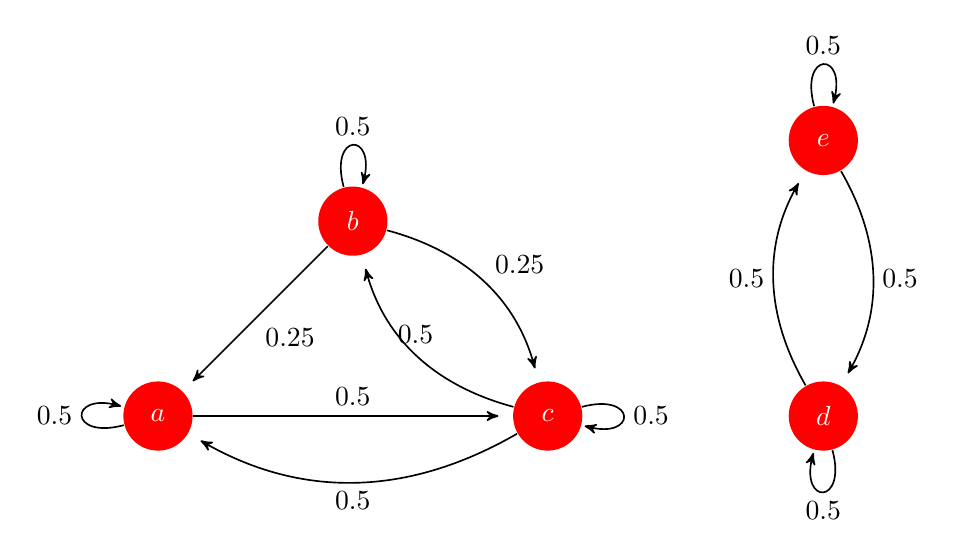
\begin{tikzpicture}[->,>=stealth',shorten >=5pt,auto,node distance=3.5cm,
                    semithick]
  \tikzstyle{every state}=[fill=red,draw=none,text=white]
  
  \node[state] (A)                    {$a$};
  \node[state]         (B) [above right of=A] {$b$};
  \node[state]         (C) [below right of=B] {$c$};
  \node[state]         (D) [right of=C] {$d$};
  \node[state]         (E) [above of=D] {$e$};
  


  \path (A) edge [loop left]  node {0.5} (A)
            edge              node {0.5} (C)
        (B) edge          node {0.25} (A)
            edge    [bend left]          node {0.25} (C)
            edge [loop above]  node {0.5} (B)
        
        (C) edge [loop right]  node {0.5} (C)
            edge [bend left] node[above] {0.5} (B)
            edge [bend left] node[below] {0.5} (A)
        
        (D) edge [bend left]   node {0.5} (E)
            edge [loop below]  node {0.5} (D)
            
        (E) edge [bend left] node {0.5} (D)
            edge [loop above] node {0.5} (E);
\end{tikzpicture}}
    \caption{A non connected graph}
    \end{subfigure}
    \hfill
    \begin{subfigure}{0.3\textwidth}
    \resizebox{\linewidth}{!}{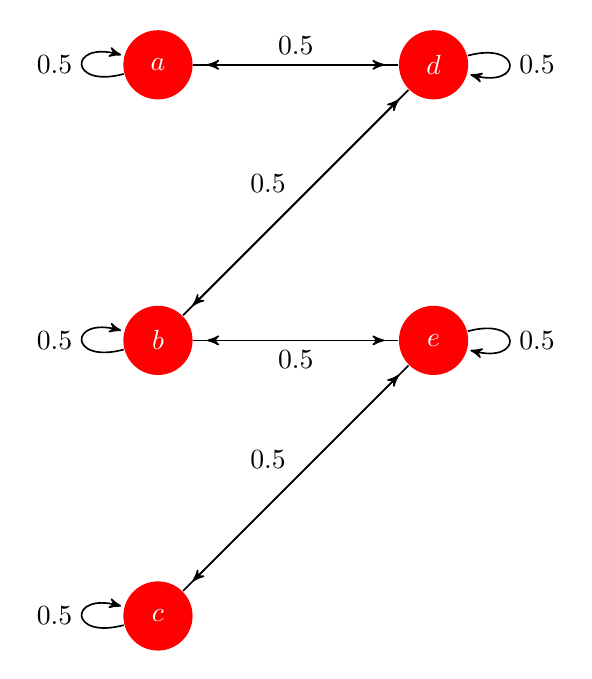
\begin{tikzpicture}[->,>=stealth',shorten >=5pt,auto,node distance=3.5cm,
                    semithick]
  \tikzstyle{every state}=[fill=red,draw=none,text=white]
  
  \node[state] (A)                    {$a$};
  \node[state]         (B) [below of=A] {$b$};
  \node[state]         (C) [below of=B] {$c$};
  \node[state]         (D) [right of=A] {$d$};
  \node[state]         (E) [below of=D] {$e$};


  \path (A) edge [loop left]  node {0.5} (A)
            edge              node {0.5} (D)
        (B) edge          node {0.5} (D)
            edge        node {} (E)
            edge [loop left]  node {0.5} (B)
        
        (C) edge [loop left]  node {0.5} (C)
            edge node {0.5} (E)
        
        (D) edge     node {} (A)
            edge     node {} (B)
            edge [loop right]  node {0.5} (D)
            
        (E) edge node {0.5} (B)
            edge node {} (C)
            edge [loop right] node {0.5} (E);
\end{tikzpicture}}
    \caption{A non aperiodic graph (bipartite graph)}
    \end{subfigure}
    
    \caption{Non ergodic markov chains}
    \label{fig:non_ergodic_markov_chains}
\end{figure}


Now let's introduce the limit distribution of a Markov Chain, that will allow us to define the importance vector.

\begin{definition}[Limit distribution of a Regular Markov Chain \cite{grinstead_snell_2006}]
Let $P$ be the transition matrix for a regular markov chain. Then, as $n \rightarrow \infty$, the powers $P^n$ approach a limiting matrix $W$ with all rows the same vector $w$. The vector $w$ is a strictly positive probability vector (all its components are strictly positive and they sum to one).

Then :
\begin{enumerate}
    \item $wP = w$ and any row vector $v$ such that $vP = v$ is a constant multiple of $w$.
    \item $P \mathbb{1} = \mathbb{1}$, where $\mathbb{1}$ is the column vector where all the coefficients are equal to 1
\end{enumerate}

The vector $w$ is called the \textbf{probability limit distribution} of the markov chain C associated with the transition matrix P. 

\end{definition}

In fact, the $P^k_{ij}$ coefficients of the successive powers of the transition matrix corresponds to the probability of a walker, starting from the node i, to get to the node j after k steps. $w$ being the rows of the matrix $\underset{k\rightarrow \infty}{lim} P^k$, the limit distribution probability coefficients $w_i$ can be interpreted as the probability to get to the node $i$ of the state graph after letting a random walker surfing on the state graph for an infinite number of steps, starting from any node in the state graph.

Hence, the definition of the probability limit distribution makes sense as a node with a high probability limit distribution value seems to attract a random walker starting from any node of the graph. 

The Perron-Frobenius Theorem is the exact transposition of the previous result to linear algebra. However, before stating the Perron-Frobenius Theorem, let's recall the definition of a left (resp right) eigenvector, as it will be heavily used in this paper.

\begin{theo}[Left/Right Eigenvector]\label{theo:limit_distrib_markov_chain}
A left (resp right) eigenvector associated with an eigenvalue $\lambda$ of a matrix $M \in \mathcal{M}_n(\mathbb{C})$ is a vector $X \in \mathbb{C}^n / \{0\}$ such that : 
\begin{equation*}
    XM = \lambda X
\end{equation*}
(respectively $MX = \lambda X$)
\end{theo}

\begin{definition-theo}[Perron-Frobenius Theorem for Positive Matrices \cite{meyer_2000}]\label{def-theo:perron-frob}
Let $M \in \mathcal{M}_n(\mathbb{C})$ be a regular matrix, ie a matrix so that 
\begin{equation*}
    \exists k \in \mathbb{N}, \mbox{ so that : } M^k_{ij} > 0, \forall (i,j) \in [1, n]
\end{equation*}

\begin{enumerate}
    \item Then, 1 is an eigenvalue of M and any other eigenvalue $\lambda$ of M is strictly smaller than 1 in absolute value, ie $\forall \lambda \in Sp(A) / 1, \|\lambda\| < 1$. 1 is called the Perron root, the Perron-Frobenius eigenvalue or the leading eigenvalue.
    \item Moreover, the Perron-Frobenius eigenvalue is simple, ie the eigenspace associated to 1 is one-dimensional.
    \item There exists a left (resp right) eigenvector $v = (v_1, \hdots, v_n)^T$ of M, associated to the Perron-Frobenius eigenvalue, with $\forall i \in [1, \hdots, n], v_i > 0$.
    \item There exists a unique left (resp right) eigenvector such that : 
    \begin{equation*}
        p M = p, \ p>0, \ and \ \|p\|_1 = 1
    \end{equation*}
    This eigenvector is called the left (resp right) Perron-vector of M.

\end{enumerate}

\end{definition-theo}

Hence, given a regular markov chain C associated with a regular matrix M, the probability limit distribution of C, is exactly the left Perron-vector of M.

Having laid the theoretical framework, we can now explain the motivations that led to the PageRank elaboration. 

\subsubsection{Classical Google PageRank}

Let $\mathcal{G}=(V,E)$ a directed graph with transition matrix P. 
If the graph $\mathcal{G}$ features dandling nodes, one transforms the matrix P into $\Bar{P}$ where 
\begin{equation*}\label{eq:dangling_nodes_free}
    \Bar{P_{i}} = \left\{
    \begin{array}{ll}
        P_{i} & \mbox{if i is not a dandling node}  \\
        (\rho_1, \hdots, \rho_n) & \mbox{if i is a dangling node}
    \end{array}
    \right.
\end{equation*} 
And where $\Bar{P_{i}}$ is the $i^{th}$ row of $\Bar{P}$ and  $(\rho_1, \hdots, \rho_n)$ is a row stochastic vector (ie $\underset{i \in [1, n]}{\sum} \rho_i = 1$). Generally, the uniform probability distribution is arbitrarily chosen \cite{langville_meyer_2004}. We will discuss the issue of dandling nodes in details in \ref{subsec:dandling}. We call the matrix $\Bar{P}$ the dangling-node free transition matrix of $C$.

In Lawrence Page $\&$ Sergey Brin's paper \cite{brin_page_1998}, the Google matrix is defined as : 

\begin{definition}[Google Matrix \cite{brin_page_1998}]
\label{def:google_matrix}
Let P be an dandling-free transition matrix associated a directed graph $\mathcal{G}$, the Google Matrix of $\mathcal{G}$ is :
\begin{equation*}
    G = (1-\alpha) P + \frac{\alpha}{n} \mathbb{1}
\end{equation*}
Where $\mathbb{1}$ is the matrix that only contains ones and $\alpha$ is a constant ($\alpha \in [0,1]$).

\end{definition}

The original intuition behind the introduction of the Google matrix is the following : let $\mathcal{G}=(V,E)$ be a directed graph representing the relations between web Pages - ie where $\forall x \in V$, $x$ is a Web Page, and ($e_{ij} \in E \leftrightarrow \mbox{ i has a link pointing towards j}$). We note $P$ the transition matrix of $\mathcal{G}$. We would like to quantify the "importance" of the nodes of the Graph - Sergey Brin and Lawrence Page chose to propagate a random walker on the Web Graph and compute the probability that the Walker get to a given node after a long time : the higher the probability is, the more importance the node has.

Thus, this amounts, formally, to define a Markov chain $C$ on the graph $\mathcal{G}=(V, E)$ whose transition matrix is $P$ and to compute the Perron vector of $P$. However, this vector does not exist necessarily and may not be unique for any transition matrix $P$ - $P$ may not be regular. Hence, the Google matrix : any Markov chain $C$ whose transition matrix is $G$ remains regular, which means one can apply the Perron-Frobenius theorem.

The Google matrix transforms the input graph by adding low-weighted edges between any pairs of nodes, making the input graph strongly connected (and thus regular). Google uses the value of 0.15 for its web search engine : this is an heuristic choice to balance fast convergence and pertinence of the results \cite{langville_meyer_2004}. In fact, the smaller the constant $\alpha$ is, the better the structure of the original graph is preserved, while the greater $\alpha$ is, the faster the PageRank converges.

Then, one can finally define the Google importance vector, using the Google matrix :
 
\begin{definition}[Google importance vector]
Let $\mathcal{G}=(V,E)$ the directed input graph. The Google importance vector is the Perron-vector of the Google Matrix of $\mathcal{G}$.

In other words, the Google importance vector is defined as being the only unit left row eigenvector associated to the eigenvalue equal to 1 of the Google Matrix. Ie I is the only vector so that:

\begin{equation}
    IG = I
\end{equation}

Since Google matrix is irreducible, it has only one eigenvalue equal to 1 and I is well defined.\\

\end{definition}

Finally, the classical PageRank algorithm performs the following steps : 

\begin{enumerate}
    \item Choose a starting vector $x^{(0)}$ (generally, $x^{(0)} = \mathbb{1}/n$ where $\mathbb{1}$ is the vector filled with ones).
    \item While $\|x^{(k)T} - x^{(k-1)T}\| < \epsilon$ (ie while the algorithm has not converged), perform the following update 
    \begin{equation*}
        x^{(k)T} = x^{(k-1)T} G
    \end{equation*}
    \item Output x.
    
\end{enumerate}

There are some ways to reduce the computational cost of the update operation : since the input transition matrix P is sparse and the Google matrix being a linear combination of P and a constant matrix - the update operation scales as $\mathcal{O}(nnz(P)) \simeq \mathcal{O} (n)$ where $nnz(P)$ is the number of non-zero components of P. See \cite{langville_meyer_2004} for more details on the explicit computation and optimisation of the classical PageRank.

\subsubsection{A few words on personalized PageRank} \label{subsec:preferential_pagerank}
Personalized PageRank was quickly introduced by L.Page and S.Brin after their pioneering work of \cite{brin_page_1998}: originally, this method was aimed to design different web Crawlers according to web Pages genres \cite{haveliwala_2003}. Indeed, personalized PageRank was designed to produce local rankings around a given node, instead of global and general graph nodes rankings. Informally, this method outputs a ranking of the most influential neighbours of a starting node.
Since its introduction, it has been applied to countless fields \cite{gleich_2015}.

Here we introduce and study the properties of this method and compare them with the original PageRank.

\begin{definition}[Personalized Google Matrix \cite{gleich_2015}]
Let $\mathcal{G}=(V,E)$ be a directed graph with transition matrix $P$ being dangling-node free (thanks to the transformation \ref{eq:dangling_nodes_free}), $\alpha \in [0,1]$ a constant and let $v \in \mathbb{R}_{+}^{|V|}, \mbox{ so that :} \sum_{i} v_i = 1$. We call $v$, the \textbf{personalization vector}. 

The \textbf{Personalized Google Matrix} of $P$ is :
\begin{equation}
    G_{pers} = \alpha P + (1-\alpha) ve^T
\end{equation}

Where $e^T=(1, \hdots, 1) \in \mathbb{R}^{|V|}$ is a row vector of ones. 

\end{definition}

Figure \ref{fig:personalized_pagerank} provides an example of construction of the personalized PageRank of a given initial weighted graph.

\begin{figure}[h!]
\centering
\begin{subfigure}{0.45\textwidth}
\centering
 \resizebox{\linewidth}{!}{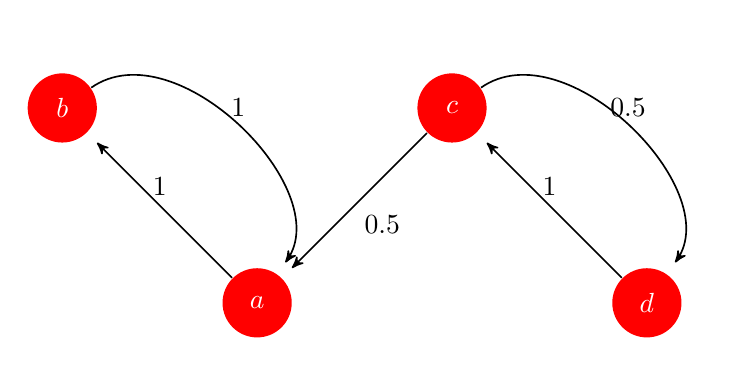
\begin{tikzpicture}[->,>=stealth',shorten >=5pt,auto,node distance=3.5cm,
                    semithick]
  \tikzstyle{every state}=[fill=red,draw=none,text=white]
  
  \node[state] (A)                    {$a$};
  \node[state]         (B) [above left of=A] {$b$};
  \node[state]         (C) [above right of=A] {$c$};
  \node[state]         (D) [below right of=C] {$d$};


  \path (A) edge              node[anchor = north, above] {1} (B)
            
        (B) edge    [bend left=80]          node[above] {1} (A)
            
        (C)  edge  node {0.5} (A)
             edge  [bend left=80] node[above] {0.5} (D)
        
        (D) edge            node[above] {1} (C);
\end{tikzpicture}}
\caption{Initial weighted graph}
\end{subfigure}%
\hfill
\begin{subfigure}{0.45\textwidth}
\centering
 \resizebox{\linewidth}{!}{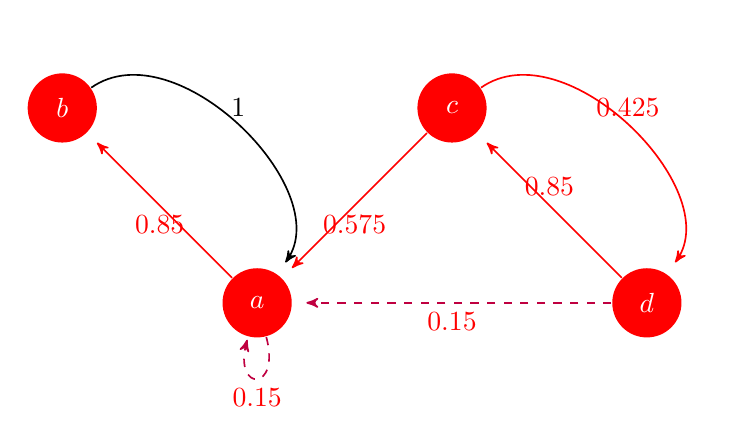
\begin{tikzpicture}[->,>=stealth',shorten >=5pt,auto,node distance=3.5cm,
                    semithick]
  \tikzstyle{every state}=[fill=red,draw=none,text=white]
  
  \node[state] (A)                    {$a$};
  \node[state]         (B) [above left of=A] {$b$};
  \node[state]         (C) [above right of=A] {$c$};
  \node[state]         (D) [below right of=C] {$d$};


  \path (A) edge [red] node[anchor = north, below, text=red] {0.85} (B)
            edge [purple, dashed, loop below] node[anchor = north, below, text=red] {0.15} (A)
            
        (B) edge  [bend left=80]          node[above] {1} (A)
            
        (C)  edge [red]  node[below, text=red] {0.575} (A)
             edge [red, bend left=80] node[above, text=red] {0.425} (D)
             
        (D) edge    [red]    node[above, text=red] {0.85} (C)
        edge    [purple, dashed]    node[below, text=red] {0.15} (A);
          
  
\end{tikzpicture}}
\caption{Final Personalized PageRank Graph.}
\end{subfigure}
\caption{An example of personalized PageRank procedure, for $\alpha = 0.15$ and $v= \delta_a$}
\label{fig:personalized_pagerank}
\end{figure}


\paragraph{Properties :} 
Let's note that $G_{pers}$ is aperiodic but not necessarily irreducible. One can prove however that $G_{pers}^k$ converges to a limit probability distribution that does not depends on the initial position of the walker, or the initial state of the markov chain \cite{gleich_2015}. In other words, the eigenspace associated with the eigenvalue 1 has a dimension exactly equal to 1.  \\
We are going to illustrate this fact with the simple example of figure \ref{fig:personalized_pagerank}. Given a Markov chain $C$ on the graph $\mathcal{G}$ of the figure, one can show that (application of the Borel-Cantelli theorem):  
\begin{equation}
    \mathbb{P}(\underset{n\in \mathbb{N}}{\bigcup}(X_n = a)) = 1
\end{equation}

This last equation can be interpreted by saying that any random Walker propagating long enough on $\mathcal{G}$ will fall on the node $a$ with a great probability that is converges to one, as the time passes by. If the walker falls on $a$, then it will remain in the connected component of $a$, which is a strongly connected component, since every node of the graph is connected to $a$. Which means that, asymptotically, the walker will have the same behaviour as another one that would have started from any node in the connected component of $a$.

This last explanation intuitively justifies the following property of a Markov chain on a Personalized Google Matrix: the non-zero limit probability distribution ($\Pi$) coefficients of the chain are those that belong in the connected components of the nodes associated with non-zero components of $v$ the personalized vector.  

\subsection{Quantum PageRank}

\subsubsection{Motivation and general considerations}

When it comes to Markov Chains, quantum computing provides an elegant framework for studying Random Walks as the different states of a random walker can be represented by a superposition of quantum states \cite{loke_tang_rodriguez_small_wang_2016}. Moreover, the properties of Quantum Random Walks are quite different from the classical random walks as state interference heavily modifies the walker probability distribution on the state graph \cite{kempe_2009}.

Indeed, some efforts \cite{paparo_2014, paparo_müller_comellas_martin-delgado_2013, sánchez-burillo_duch_gómez-gardeñes_zueco_2012, loke_tang_rodriguez_small_wang_2016, garnerone_zanardi_lidar_2012, paparo_martin-delgado_2012} have already been made to try and apply quantum computing principles to Pagerank computation. These results were rather interesting as they seemed to reveal the graph structure more clearly, outperforming the classical PageRank on several counts. In fact, discrete quantum rankings discriminate secondary hubs more clearly and the Quantum based methods can differentiate between hierarchical, scale-free and Erdős–Rényi networks \cite{paparo_2014, paparo_müller_comellas_martin-delgado_2013, loke_tang_rodriguez_small_wang_2016}.

Besides, some methods provide polynomial computational savings over its classical counterpart \cite{garnerone_zanardi_lidar_2012}, the Quantum MCMC method also provides a significant computational improvement. However, when it comes to discrete quantum walk based solutions from \cite{paparo_2014, paparo_müller_comellas_martin-delgado_2013, paparo_martin-delgado_2012}, these algorithms were designed to produce classical simulations of discrete quantum walks, hence does not provide significant improvements in comparison with the classical random walk based solutions. Nonetheless, this method seem to scale quite well to large networks \cite{loke_tang_rodriguez_small_wang_2016}. We will analyse more deeply the convergence and the performances of these algorithms in \ref{subsec:performanceIssues}.

\subsubsection{Szegedy's Discrete Quantum Walk}
\label{subsubsec:szegedy_discrete_quantum_walk}

For a classical Markov Chain represented by the graph G = (V, E) and the probability transition matrix P, a transition step establishes the map defined on the nodes of the graph G, $i\in V$: 
\begin{equation*}
    i \rightarrow \underset{j \in V}{\sum} P_{ij} j
\end{equation*}

Hence, a quantum equivalent of the last mapping may be :
\begin{equation*}
    \ket{i}\ket{0} \rightarrow \underset{j \in V}{\sum} \sqrt{P_{ij}} \ket{i} \ket{j}
\end{equation*}

Here we added the ancilla qBit $\ket{0}$ so that the last equation becomes reversible - every quantum transformation on a given state (except for the measurement operation) must be reversible.

Thus, this method allows one to quantize a Markov Chain, ie to transpose the classical representation of the Markov Chain into a quantum equivalent. This is called the Szegedy's procedure of quantization \cite{szegedy}.

The difference between the classical and quantum walks unveils after letting the walker propagate for a few steps : in the quantum framework the states interferes which heavily modifies the walker's presence probability distribution. The common example of a quantum walk on a line is well described in \cite{kempe_2009}.

Using Szegedy's procedure, one can build quantum walks to simulate the propagation of a quantum walker on the graph G - in fact, this quantization method is rather interesting as one can then rely on Szegedy's theorem that describes thoroughly the eigenspaces of a specific walk operator W :

\begin{theo}[Szegedy's theorem \cite{szegedy}]
Let $\mathcal{G}=(V,E)$ a graph, and P the probability transition matrix associated with a random walk on $\mathcal{G}$. Moreover, let $\mathcal{A}$ and $\mathcal{B}$, the two spaces defined by :

\begin{equation*}
    \mathcal{A} = Span\{\sum_y \sqrt{P_{xy}} \ket{x} \ket{y} : x \in V\}
\end{equation*}

\begin{equation*}
    \mathcal{B} = Span\{\sum_x \sqrt{P_{yx}} \ket{x} \ket{y} : y \in V\}
\end{equation*}

Then, let $W := ref(\mathcal{B})\ o \ ref(\mathcal{B)}$ and $D_{x,y} := \sqrt{P_{x,y}P_{y,x}}, \forall (x,y) \in V^2$ - its eigenvalues being $cos(\theta_1, \hdots, \theta_n)$ (see \cite{szegedy} for the justification of why the singular values of D are at most one) - one can say the following about the eigenvalues of $U^2$ : 

\begin{enumerate}
    \item On $\mathcal{A} \bigcup \mathcal{B}$ the eigenvalues of $W$ that have non-zero imaginary part are exactly $e^{-2i\theta_1}, e^{+2i\theta_1}, \hdots, e^{-2i\theta_n}, e^{2i\theta_n}$
    \item On $\mathcal{A} \bigcap \mathcal{B}$, $W$ acts as the identity - this space coincides with the set of eigenvectors of $D$ with singular value 1
    \item On $\mathcal{A} \bigcap \mathcal{B}^{\perp}$ and on $\mathcal{A}^{\perp} \bigcap \mathcal{B}$, $W$ acts as a reflection on the center (ie as -Id).
    \item On $\mathcal{A}^{\perp} \bigcap \mathcal{B}^{\perp}$, $W$ trivially acts (acts as the identity).
\end{enumerate}

\end{theo}
 
The operator W defined above is usually called the Walk operator : to simulate a step of the quantum Walk, one has to apply W to the current state of the walker. This theorem is fundamental for most of the Quantum algorithms relying on Szegedy's quantization procedure.

\subsubsection{Discrete Quantum PageRank} 
\label{subsubsection:Paparo_quantum_walk}
In \cite{paparo_martin-delgado_2012} the authors use Szegedy’s procedure \cite{szegedy} to Quantize markov chains and then apply a quantum walk, finding eigenvalues and eigenvectors of a specific Quantum diffusion operator, then extracting the value of the mean PageRank in time. In fact, \cite{paparo_martin-delgado_2012}, introduced a classical algorithm to compute its Quantum PageRank, estimating that simulations on a Quantum Computer were not feasible in a near future (the algorithm was introduced in 2012). Thus, the main contribution of this paper lies in the study of the influence of Quantum Probability interference stemming from Quantum Random Walks on the final score of the PageRank.

The Quantum walk takes place in the Hilbert Space $\mathcal{H}^{N^2} = \mathcal{H}^{N} \otimes \mathcal{H}^{N}$, which is spanned by vectors $\ket{j,k}$ representing an edge from node j to node k of the input directed graph.

Paparo \cite{paparo_martin-delgado_2012} starts the walk from the state :
\begin{equation*}
    \frac{1}{\sqrt{N}}\ket{\psi_j}
\end{equation*}
Where :
\begin{equation*}
    \ket{\psi_j} := \ket{j} \otimes \sum_{k=1}^N \sqrt{G_{kj}} \ket{k} = \sum_{k=1}^N \sqrt{G_{kj}} \ket{j,k}
\end{equation*}

The $G_{kj}$ being the coefficients of the Google matrix obtained from the input graph.
This $\ket{\psi_j}$ state represents the superposition of edge states $\ket{j} \ket{k}$ outgoing from the node j.

Then, \cite{paparo_martin-delgado_2012} defines the step operator as  $\hat{U} := \hat{S} (2 \hat{ \Pi} - \hat{{1}})$. Where $\hat{S}$ is the swap operator : 
\begin{equation*}
    \hat{S} := \sum_{j,k=1}^N \ket{j,k}\bra{k,j}
\end{equation*}
and $\hat{\Pi}$ is the projector on the space spanned by the $\ket{\psi_j}$, ie $\hat{\Pi} := \sum_{j=1}^N \ket{\psi_j}\bra{\psi_j}$. $\hat{1}$ is the identity operator.

These two operators act on the state space to propagate the Quantum Walk. In fact, $\hat{U}$ is then the composition of a reflection around the space spanned by the $\ket{\psi_j}$ - to simulate the random part of the walk, this is analogous to the coin-flip step in the simple line Quantum Walk - followed by a step which reverses the edges of the directed walk graph.

Hence, to preserve the directedness of the walk, one rather needs to use the two-step evolution operator : 
\begin{equation*}
    \hat{U}^2 := (2 \hat{S} \hat{\Pi} \hat{S} - \hat{1})
\end{equation*}

Which means that the edges are reversed twice and the input graph is still directed.

The introduction of these operators rely on Szegedy's theorem. Indeed, the walk operator W is exactly $U^2$ : applying $U^2$ to a quantum walk state amounts to composing two reflections - the first one on the space $Span\{\sum_y \sqrt{P_{xy}} \ket{x} \ket{y} : x \in V\}$; the second one on the space $Span\{\sum_x \sqrt{P_{yx}} \ket{x} \ket{y} : y \in V\}$ - which is exactly how W is defined. This theorem allows to reduce the number of computations since $U^2$ acts non trivially solely on a \textbf{dynamical subspace} of dimension 2N (where N is the number of nodes of the walk) while it admits $N^2$ eigenvalues.

Then, computing the random walk for a given time only amounts to applying the two-step evolution operator several times to an initial state from the \textbf{dynamical subspace}. The instantaneous discrete quantum PageRank is the probability that the walker ends its walk at the node $i$, after $t$ steps :
\begin{equation*}
    I_d(\ket{i}, t) = \bra{\psi_0} \hat{U}^{\dagger 2t} \ket{i} \bra{i} \hat{U}^{2t} \ket{\psi_0}
\end{equation*}

This instantaneous PageRank does not converge in time (ie $\underset{t\rightarrow\infty}{lim} I_d(\ket{i}, t)$) because of the quantum interference effect on the walk we mentioned earlier - however the mean of the instantaneous PageRanks converges for large enough $t_{max}$.

Hence, the global PageRank is defined as : 
\begin{equation*}
    I_{TA}(\ket{i}) := \braket{I_d(\ket{i}, t}= \frac{1}{t_{max}} \sum_{t=0}^{t_{max}-1} I_d(\ket{i}, t)
\end{equation*}

In practice, \cite{paparo_martin-delgado_2012} use the following closed form expression to compute the instantaneous pagerank on a classical computer : 
\begin{equation*}
    I_q(\ket{i}, m) = \| \underset{\mu}{\sum} \mu^{2m} \braket{i|\mu} \braket{\mu|\psi(0)} \|^2
\end{equation*}
Where $\ket{\mu}$ and $\mu$ are the eigenstates and eigenvalues of $U^2$ that lie on the dynamical subspace and $\psi(0)$ and initial state that lie on the dynamical subspace.

Hence, the Quantum PageRank Protocol \cite{paparo_martin-delgado_2012}:
\begin{enumerate}
    \item Write the Google Matrix for the input graph
    \item Write the matrix D (see Szegedy's theorem) and compute its eigenvalues + eigenvectors
    \item Find the eigenvectors and eigenvalues of $U^2$ in the dynamical subspace $H_dyn$
    \item Compute the instantaneous Quantum PageRanks and the mean value of the Quantum PageRanks starting from $\ket{\psi_0} = \frac{1}{\sqrt{N}} \sum_{i=1}^N \ket{\psi_j}$
\end{enumerate}


One again, this method is used to simulate a discrete Quantum Walk on a classical computer. Even though this approach is interesting as it allows one to study the influence of Quantum Interference on importance rankings, it does not provide a Quantum algorithm to solve the problem as it relies on classical computation.

\subsubsection{Continuous Quantum PageRank}

Continuous Time Quantum PageRanks have been introduced by \cite{sánchez-burillo_duch_gómez-gardeñes_zueco_2012}. Their approach is similar to the one of \cite{paparo_martin-delgado_2012} as they solely aim at studying Quantum Walk effects on the computation of PageRank rather than trying to improve its complexity - their paper provides a Classical computational algorithm based on Quantum formalism. Still, the quantum formalism is interesting as it differs on several grounds from the method used by \cite{paparo_martin-delgado_2012}. 

Indeed, one of the most interesting contributions of \cite{sánchez-burillo_duch_gómez-gardeñes_zueco_2012} is the use of the Lindblad equation to take into account the PageRank graph directedness into the continuous time quantum Walk. This technique is inspired by Quantum Stochastic Walks which were introduced by \cite{whitfield_rodríguez-rosario_aspuru-guzik_2010} in 2010. In other words, the evolution of the global system is governed by :
\begin{equation}\label{lindblad_general_form}
\partial_t \rho(t) = -i (1- \beta) [\hat{H}, \rho] + \beta \sum_{i,j} G_{ij} (\hat{L}_{ij} \rho \hat{L_ij}^{\dagger} - \frac{1}{2}\{\hat{L}_{ij} \hat{L}_{ij}^\dagger, \rho\})
\end{equation}
Where :
\begin{itemize}
    \item $\rho(t)$ is the system density matrix, initialized as $\rho_{ij}(t=0) = \frac{\delta_{ij}}{N}$ where $\delta_{ij} = 1 \mbox{ iff } i=j$
    \item $\hat{L}_{ij} = \ket{i}\bra{j}$ is a basis of unitary vectors of the space that contains $\rho$.
    \item $\hat{H}$ is the undirected adjacency matrix of the input graph
    \item $G$ is the Google Matrix
    \item And $\beta$ is a constant so that $\beta \in [0,1]$
\end{itemize}

The original purpose of this equation is to model open Quantum Systems by combining a pure Quantum effect and an environment perturbing effect - the first part of the right member : $-i [\hat{H}, \rho]$ accounts for the Quantum effect (it is the right member of Schrodinger's equation) and the second part, $\sum_{i,j} G_{ij} (\hat{L}_{ij} \rho \hat{L_ij}^{\dagger} - \frac{1}{2}\{\hat{L}_{ij} \hat{L}_{ij}^\dagger, \rho\})$, accounts for the environmental perturbations. Thus $\hat{L_{ij}}$ presents the effect of environmental perturbations on each state $\ket{i}\ket{j}$. The parameter $\beta$ models the degree of coupling between Pure Quantum Effects and Environmental Coupling.

Here this equation is used to solve the issues aforementioned in \ref{subsubsec:szegedy_discrete_quantum_walk} : Pure Quantum evolution processes need to feature reversible operations, hardly compatible with the directed structures of the input graphs, in addition to preventing the global process to converge (as duly noted in section \ref{subsubsection:Paparo_quantum_walk}) ; here open quantum processes are used to take into account graph directness as an environmental perturbation which eventually allow convergence towards an limit stationary distribution. In other words, introducing environmental effects to an Open Quantum System yields an irreversible evolution which may imply the convergence of the system to a limit state. Several analogies to the physics world can be used to better understand Open Quantum Systems : idealised perpetual pendulum motion can be seen as a "pure pendulum system" which becomes an open system losing energy when friction is taken into account ; in thermodynamics, this notion of closed and open systems is also heavily used.

A thorough introduction (and derivation) for the Lindblad master equation can be found here \cite{manzano_2020}.

In their paper \cite{sánchez-burillo_duch_gómez-gardeñes_zueco_2012}, Sánchez-Burillo et all prove that a $\rho(t)$ following \eqref{lindblad_general_form} converges to a unique stationary distribution if $\beta \neq 0$. In this case, the stationary distribution is a combination of Pure quantum walk effects and classical walk effects (the proportion of each effect being determined by the value of $\beta$) which unveils quite interesting properties on nodes rankings, especially for low ranked nodes which are much more affected by the quantum walk effects. 

Finally, Sánchez-Burillo et all compute each PageRank by solving numerically the differential equation $\delta_t \rho(t) = \mathcal{L}\rho$, where $\mathcal{L}$ is identified using \eqref{lindblad_general_form}.\\
$\mathcal{L}$ being a linear (respectively to $\rho$) time independent operator, until convergence to a stationary distribution. Hence, computing a classical solution of a quantum modeled problem.

Please note that Sánchez-Burillo et all note that other methods can be used to solve the Continuous Quantum PageRank such as Quantum Adiabatic Computation that was used in \cite{garnerone_zanardi_lidar_2012}. Quantum Adiabatic Computation being polynomially equivalent to Circuit-based quantum Computing \cite{aharonov_dam_kempe_landau_lloyd_regev_2008}, these results provide a first algorithm to compute PageRank on Quantum computers.

\subsection{Convergence analysis and performance issues.}
\label{subsec:performanceIssues}

To analyse the performances of the algorithms described above, it is important to make a clear distinction between \textit{classical computed classical-based algorithms}, \textit{classical computed quantum-based algorithms} and \textit{quantum computed quantum-based algorithms}. Indeed, classical-computed quantum-based algorithms are not firstly designed for computing efficiency: in fact, the main contribution of these algorithms is to study the effects of Quantum interference on the PageRank rankings \cite{paparo_müller_comellas_martin-delgado_2013, sánchez-burillo_duch_gómez-gardeñes_zueco_2012}. 

Nonetheless, let us note the computational improvement provided by the Continuous Quantum PageRank introduced in \cite{sánchez-burillo_duch_gómez-gardeñes_zueco_2012} over the classical PageRank : indeed, the authors of the paper have noted a constant factor performance improvement of the Quantum PageRank for a given value of the parameter $\beta$. Sánchez-Burillo et all claim that this speedup does account for a positive interference effect between the combination of Classical and Quantum Random Walks.

In fact, only \cite{garnerone_zanardi_lidar_2012} seem to provide a computational quantum method to solve the PageRank thanks to Quantum Adiabatic Computation. The authors used numerical simulations to derive a Quantum Pagerank computation complexity in $\mathcal{O}(polylog(n))$ for the $log(n)$ most influential nodes of the input graph. However, theoretical complexity results were not provided in this work, which is quite common as forecasting Quantum Adiabatic performances before computational time is non-trivial in comparison to Circuit based quantum algorithms.

\subsubsection{Convergence speed comparison}
It is possible to derive several results regarding PageRank's algorithm converging speed, one of the most notable results which we will prove using complexity theory in \ref{section:theoretical_proofs_of_convergence} (one would need to introduce several concepts of Spectral Graph Theory before), states that the original PageRank algorithm converges in $\mathcal{O}(1)$ time, which makes the complexity of the classical PageRank algorithm $\mathcal{O}(n)$ using optimization methods for sparse matrices.

Even though \cite{sánchez-burillo_duch_gómez-gardeñes_zueco_2012} introduced a Quantum algorithm enhancing computation speed in comparison with the classical PageRank, the complexity remains linear with the size of the input matrix.

The algorithm introduced by Paparo et all  \cite{paparo_martin-delgado_2012} does not significantly improve the computation speed.

One can find an instance of classical distributed algorithm which may be used to compute PageRank in $\mathcal{O}(log(n))$ in \cite{sarma_molla_pandurangan_upfal_2013}, however this distributed algorithm settles in the very specific environment of a distributed network of computing nodes, which is rather restrictive in comparison to our general setting.

Figure \ref{fig:pagerank_computation} summarize the above discussion :

\begin{figure}[h!]\label{fig:pagerank_computation}
    \centering
    \begin{tabular}{|c|c|c|c|}
    \hline
    Computation Type & Method name & Complexity \\
    \hline \hline
    Classical Computing & Classical PageRank & $\mathcal{O}(n)$\\ \hline
    Distributed Computing & Distributed PageRank (for intelligent nodes) & $\mathcal{O}(log(n))$ \\ \hline
    Classical Computing & Discrete Quantum PageRank \cite{paparo_martin-delgado_2012} & $\mathcal{O}(poly(n))$\\ \hline
    Classical Computing & Continuous Quantum PageRank \cite{sánchez-burillo_duch_gómez-gardeñes_zueco_2012} & $\mathcal{O}(n)$\\ \hline
    Adiabatic Quantum Computing & Adiabatic Continuous Quantum PageRank \cite{garnerone_zanardi_lidar_2012} & $\mathcal{O}(log(n))$ (experimental)\\
    \hline
\end{tabular}

    
    \caption{Comparison of the existing PageRank computation methods}
    \label{fig:pagerank_computation}
\end{figure}

\subsubsection{Ranking Performance results}

The algorithm introduced by Paparo et all in 2012 is interesting in the sense that it provides better ranking performances than the classical algorithm \cite{paparo_martin-delgado_2012, paparo_müller_comellas_martin-delgado_2013, paparo_2014}. In fact, it exhibits a different behavior and different performance improvements for different types of input graph structures : for scale-free networks, the quantum algorithm highlights better the secondary hubs, and seem to discriminate low-ranked nodes more precisely ; for hierarchical graphs, the algorithm separates hierarchical levels more clearly and achieve  better performances in comparison with the classical PageRank algorithm when it highlights the connectivity structure of each hierarchy level ; finally, the algorithm succeeds in detecting whether a graph belongs to the Erdös-Rényi type or the scale-free type. Discrete Quantum PageRank seems more robust to the $\alpha$ parameter variation (see definition \ref{def:google_matrix}).

However, this algorithm presents an increased sensitivity to coordinated attacks on the nodes (if an important node of the input graph is removed, the subsequent ranking varies more in the Discrete Quantum PageRank setting rather than in the classical PageRank algorithm).

The Continuous PageRank algorithm \cite{sánchez-burillo_duch_gómez-gardeñes_zueco_2012} also features improved ranking performances than the classical algorithm. In fact, continuous PageRank seems to give less importance to nodes connected to highly influential hubs and increase the score of nodes connected to other locally influential nodes. This may be explained, qualitatively, by the fact that hubs concentrate a great amount of nodes which tend to dilute the hub score across its nodes ; whereas a highly influential local hub has a low node density which makes each node have a higher score.

\subsection{Our Contributions}
This paper contributions are threefold :

\begin{itemize}
    \item Our first contribution consists in applying the Spectral Graph Theory Framework to the PageRank theory to generalize the scope of the original algorithm. To this effect, we introduce a generalized PageRank ranking based on the Directed Graph Fourier Transform which allows producing more pertinent rankings by filtering the spectrum of the Google Graph. We then introduce an extension of Google matrices that can be used conjointly with the generalized PageRank to fully exploit its versatility.
    
    \item Then we introduce one of the first Quantum Based Algorithms to perform a wide range of graph signal filters and Kernel-based signal production with a low gate complexity. This algorithm relies heavily on the Quantum Singular Value Transformation framework that stems from the recent field of Quantum Signal Processing. We then provide an application example of this Quantum Algorithm to our generalized PageRank model.
    
    \item Finally, we introduce a Quantum Circuit based equivalent of the Adiabatic Quantum algorithm introduced by \cite{garnerone_zanardi_lidar_2012}. This Circuit prepares the state $\ket{\pi}$, $\pi$ being the classical Google Importance vector, simulating an Hamiltonian for time $\mathcal{O}(\frac{log(N)}{\epsilon})$. 
    
\end{itemize}

\section{A thorough introduction to the Spectral Graph Theory for directed graphs.}
\label{sec:SGTIntro}

Spectral graph theory (SGT) is a new mathematical theory that aims to adapt signal processing to graph theory : SGT studies the influence of Graph Fourier Transform on graph properties \cite{shuman_narang_frossard_ortega_vandergheynst_2013}. This theory has numerous applications and consequences on the study of graphs : from Machine learning and Computer Graphics to pure mathematics. See \cite{chung_1997, ricaud_borgnat_tremblay_gonçalves_vandergheynst_2019, shuman_narang_frossard_ortega_vandergheynst_2013, sevi2019} for instance. In the following section, we aim at presenting several fundamental results and notions from this theory that will be useful to generalise the previous PageRank methods from \ref{sec:previousResults}. 

\subsection{From Classical Fourier Analysis to SGT}

\paragraph{Reminders of classical one-dimensional Fourier Analysis:} \label{par:classical_fourier_analysis}
Any integrable function, $f : \mathbb{R} \rightarrow \mathbb{C}$, can be expanded on the Fourier orthonormal basis of vectors $(x \rightarrow e^{2i\pi x y})_{y \in \mathbb{R}}$ thanks to the identity :

\begin{equation}
    \forall x \in \mathbb{R}, f(x) = \int_{y \in \mathbb{R}} \hat{f}(y) e^{2i\pi x y} dy
\end{equation}

And the expansion coefficients, which defines a function called the Fourier Transform of f, noted $\hat{f}$, follow the identity:
\begin{equation}
    \forall y \in \mathbb{R}, \hat{f}(y) = \int_{x \in \mathbb{R}} f(x) e^{-2i\pi x y} dx
\end{equation}

Thus, one may interpret the Fourier expansion of f as a summation over a continuous basis of waves, $(x \rightarrow e^{2i\pi x y})_{y \in \mathbb{R}}$, whose coefficients are the values of the Fourier transform of $f$, named $\hat{f}$.

This parallel to classical Fourier Analysis is interesting, as it allows to better understand the main ideas of SGT: study functions on graphs as a sum of waves that propagate at a given frequency. Indeed, SGT aims at defining a Fourier Graph Basis, whose elements can be interpreted as waves varying at a given frequency, that can be used to expand any function - or \textit{signal} - on a given graph.

Fourier Analysis is closely related to the Laplacian Operator $\Delta$. Indeed, the Fourier expansion draw its origins from the study of the solutions of the Heat Equation by Joseph Fourier - to which \cite{ricaud_borgnat_tremblay_gonçalves_vandergheynst_2019} dedicate their retrospective paper on SGT advances. 

Indeed, in the simplified one-dimensional bounded classical setting, the heat equation can be written as : $\partial_t u = \alpha^2 \Delta u$, where $u \in \mathcal{C}([0,L]\times \mathbb{R}^+) ; (x,t) \rightarrow u(x,t)$ is the heat distribution function and $\alpha$ is a constant. One chooses the case where initial condition can be written as an Fourier series, ie $u(x, 0) = \frac{c_0}{2} + \sum_{n=0}^{\infty} c_n cos(\frac{\pi n x}{L})$ and Neumann Boundary conditions ($\partial_t(x,t)=0 \ ; \forall x \in B$, where B is the boundary of the problem.
\\
The solution of the heat equation can then be written as :
\begin{equation}\label{eq:heat_eq_classical_solution}
    u(x,t) = \frac{c_0}{2} + \sum_{n=0}^{\infty} c_n e^{\frac{-n^2 k^2 \pi^2 t}{L^2}} cos(\frac{\pi n x}{L})
\end{equation}

It is the decomposition on the discrete Fourier basis of eigenvectors $x \rightarrow cos(\frac{\pi n .}{L})$ of the one-dimensional classical Laplacian, whose respective eigenvalues are $e^{-\lambda_n t} c_n$ with $\lambda_n = \frac{n^2 k^2 \pi^2}{L^2}$. Hence, the solution to the heat equation is an infinite sum of Fourier waves whose amplitudes decrease exponentially as their frequencies increase.

Thus, an intuitive way to define a Fourier Graph Basis is to define first a graph Laplacian operator, then rely on the eigendecomposition of the Laplacian to define the Graph Fourier Transform \cite{shuman_narang_frossard_ortega_vandergheynst_2013, ricaud_borgnat_tremblay_gonçalves_vandergheynst_2019}.

Please note that there exists a general solution of the heat equation on an unbounded domain, that does not suppose the initial condition to be Fourier expandable - this solution uses the Fourier Transform introduced above. However, getting into the solution details will make us getting too far away from our main purpose : providing an intuition of the reasons that will lead us to use SGT for generalizing the PageRank.

However, one may remark that the $((x \rightarrow e^{2i\pi x y })_{y\in \mathbb{R}})$ are eigenvectors for the one-dimensional Laplacian operator $\Delta = \partial^2_{x}$, associated with the eigenvalue $(2\pi y)^2$ : 
\begin{equation}
    - \Delta (e^{2i\pi x y}) = - \partial^2_x e^{2i\pi x y} = (2\pi y)^2  e^{2i\pi y x }
\end{equation}
One can associate a frequency to each wave - $x \rightarrow e^{2i\pi x y }$ - which is the eigenvalue $(2\pi y)^2$ : when y is close to 0 (low frequencies), the wave displays slow oscillations ; and when y is far from 0, the wave oscillates rapidly.


\paragraph{Transposition of classical Fourier Analysis to Spectral graph Theory.} 
From the previous paragraph, one can see that to adapt Fourier Analysis to Spectral Graph Theory, one must introduce : 
\begin{itemize}
    \item \textit{Graph Signals} : given $G=(V,E)$ a graph, a signal $\phi$ on G is a function $\phi : V \rightarrow \mathbb{C}$
    
    \item \textit{A Graph Laplacian}
    
    \item \textit{A Graph Fourier Transform}, and the associated \textit{Graph Fourier basis}
    
    \item \textit{Wave frequencies} associated with the vectors of the \textit{Graph Fourier basis}.
\end{itemize}

We have chosen to introduce Spectral Graph Theory (SGT) for Directed Graphs through the study of Markov Chains, in a similar fashion as \cite{sevi2019}. Indeed, previous results from \cite{sandryhaila_moura_2014,  sardellitti_barbarossa_lorenzo_2017} yielded interesting yet less exhaustive extensions of the theory as they introduce either non-closed form expressions for \textit{Graph Fourier Transform} \cite{sardellitti_barbarossa_lorenzo_2017}, or does not incorporate well previous works on undirected graphs -\cite{sandryhaila_moura_2014} providing a whole different approach to SGT.

What is more, \cite{sevi2019} approach is interesting as it incorporates the Random Walk framework that was already introduced in \ref{subsubsec:Theo_prepreq}, and nicely defines the Graph Fourier Transform within this context.

Please let us remind (see \ref{ergodic_regular_markov}) that \cite{sevi2019} uses the term of \textit{ergodic Markov Chain} to designate \textit{regular Markov Chains}. These two concepts are equivalent considering that we assume the studied Markov Chain state spaces are finite.

\subsection{Introduction to Spectral Graph Theory for directed graphs}

\subsubsection{Lazy and reversible Markov Chains.}
In the framework introduced by \cite{sevi2019}, Graph Fourier Transform are defined for regular random walks. Two Random walk extensions are used by \cite{sevi2019} : \textit{lazy random walk} and \textit{reversible random walk}.

\begin{definition}[Lazy Markov Chain \cite{sevi2019}]
Let $C$ be a Markov Chain on a directed graph $G$ with transition matrix $P$. One defines the Lazy Markov Chain version of $C$, $\Tilde{C}$ with transition matrix $\Tilde{P}$ by :
\begin{equation}
    \Tilde{P} = \frac{Id + P}{2}
\end{equation}
Where $Id$ is the identity matrix.

\end{definition}

The \textit{lazy Markov Chains} are often used as a mean to overcome periodicity issues for Markov Chains. Indeed, Lazy Markov Chains are aperiodic, which then guarantees the convergence of any irreducible walk to a unique stationary distribution. Making a Markov Chain lazy amounts to adding self looping edges to the former Markov Chain state graph.

One can define generalized Lazy Markov Chain by adjusting the barycenter between the Identity Matrix and P, the chain transition matrix. Namely, given $\gamma \in [0,1]$, the $\gamma-$generalized lazy Markov Chain version of $CC$, $\Tilde{C_{\gamma}}$ is defined by : 
\begin{equation}
    \Tilde{P_\gamma} = (1-\gamma) P + \gamma Id
\end{equation}

The generalized Lazy Markov Chain transition probability versions $\Tilde{P}$ of the original chain $P$ share the same eigenspaces - which is convenient since SGT bases its results on the study of eigenspaces of walk operators.

\begin{definition}[Time-Reversed Markov Chain \cite{sevi2019}]\label{def:time_reversed_chain}
Let $C$ be a Markov Chain on a directed graph $G=(V,E)$ with transition matrix $P$. Let $M>0$ be a positive integer, one defines the time-reversed Markov Chain $C^* = (C_n^*) = (C_{M-n})$, for $n = 0, \hdots, M$, with transition matrix $P^*$ as :
\begin{equation}
    \forall (x,y) \in V^2 ; P^*_{x,y} = \mathbb{P}(X^*_{n+1} = y | X^*_n = x) = \frac{\mathbb{P}(X_{M-n-1} = y)}{\mathbb{P}(X_{m-n}=x)} P_{y,x}
\end{equation}

If $C$ is regular with a limit probability distribution $\pi$, the time reversed Markov chain $C^*$ is also regular with stationary distribution $\pi$ and :

\begin{equation} \label{eq:reversed_markov_chain}
    \forall (x,y) \in V^2 ; P^*_{x,y} = \mathbb{P}(X^*_{n+1} = y | X^*_n = x) = \frac{\pi(y)}{\pi(x)} P_{y,x}
\end{equation}

Which is equivalent to the Matrix equation :

\begin{equation}
    P^* = \Pi^{-1} P^T \Pi
\end{equation}

Where $\Pi = diag(\pi(x)_{x\in V})$

\end{definition}

One possible interpretation of time reversed Markov Chains stems from the identity \ref{eq:reversed_markov_chain}. Multiplying by $\pi(x)$, one gets :

\begin{equation}\label{eq:power_equilibrium}
    \forall x,y \in V, \ \pi(x) P^*_{x,y} = \pi(y) P_{y,x}
\end{equation}

This equation can be interpreted as a power flow equilibrium. Indeed, drawing a parallel with heat propagation, $\pi(x)$ and $\pi(y)$ can be seen as temperatures, $P_{x,y}$ and $P^*_{y,x}$ as heat fluxes. Then the previous equilibrium states that the heat flowing from the node $x$ to the node $y$ should be equal to the heat coming form the node $y$ to the node $x$.

Using time-reversed Markov Chains, one can define reversible Markov Chains :

\begin{definition}[Reversible Markov Chain \cite{sevi2019}]
Let $C$ be a Markov Chain. $C$ is said reversible is $C = C^*$
\end{definition}

Time-reversed Markov chains transition matrices have display several peculiar algebric behaviours, that we will describe throughout this paper. Let's introduce one first property of time-reversed Markov chains:

\begin{propriete}[Time-Reversed Markov Chains are adjoint operators \cite{sevi2019}]
    Let $C$ be a regular Markov Chain on graph $G=(V,E)$ with transition matrix $P$ and stationary distribution $\pi$ ; $f, g \in \mathbb{C}^{V}$ be two signals on G.
    
    One can define a scalar product - $<.>_{\pi}$ - on $l^2(V, \pi)$, by : 
    
    \begin{equation}
        <f,g>_{\pi} = \sum_{v \in V} \hat{f(v)}g(v)\pi(v)
    \end{equation}

Then, $P^*$ is the adjoint of $P$ for the scalar product $<.>_{\pi}$

\end{propriete}

One will end this section by introducing Markov Chain additive Reversibilization, which may be a used to make a Markov chain reversible (and consequently irreducible).

\begin{definition}[Markov Chain Additive reversibilisation \cite{sevi2019}]
Let $C$ be a Markov Chain on $G=(V,E)$ with $P$ its probability transition Matrix. 

The additive reversibilization of $C$ - $\hat{C}$ - is the Markov Chain whose probability transition Matrix is defined by :

\begin{equation}
    \hat{P} = \frac{P + P^*}{2}
\end{equation}

In a similar way as the generalized Lazy Walks, given a parameter $\alpha \in [0,1]$ one can define a generalized Reversibilization of $C$ - $\hat{C_\alpha}$ by the transition matrix :

\begin{equation}
    \hat{P_\alpha} = (1-\alpha) P + \alpha P^*
\end{equation}

The additive reversibilization process makes a Random Walk reversible iff $\alpha = \frac{1}{2}$

\end{definition}

The additive reversibilization process adds reversible edges to the original graph G. The interpretation we've provided above may be used here to better understand the generalized reversibilization process : the $\alpha$ parameter may be used to introduce a bias between power flow coming from the original edges over the reversed ones. 

Let's precise that, if $P$ is regular, all the $\hat{P}_\alpha$ for $\alpha \in [0,1]$ share the same stationary distribution but do not have the same eigenspaces.

\subsubsection{Graph Laplacians}

H. Sevi et all \cite{sevi2019} defines three different Laplacians on directed graphs : the \textit{normalized graph Laplacian}, \textit{the Random Walk Lalacian} and the \textit{Combinatorial Laplacian}. We will mostly use the Random Walk Laplacian in this paper, however the two other definitions of random walk Laplacians are most commonly used for undirected graphs. In fact, the definition of undirected graph Laplacians, may be obtained directly by manipulating the heat propagation equation on graphs - such a derivation that can be found in \cite{ricaud_borgnat_tremblay_gonçalves_vandergheynst_2019}.

\begin{definition}[Random Walk Laplacian]
Let $C$ be a regular Markov chain on $G=(V,E)$ with probability transition matrix $P$. The Random Walk Laplacian of $C$ is defined by:
\begin{equation}
    \mathcal{L}^{rw} = I - \hat{P}
\end{equation}

\end{definition}

With $\hat{P}$ the reversibilized transition matrix of the regular Markov chain $C$.

One can also define a generalized Random Walk Laplacian, $\mathcal{L}^{rw}_\alpha = I - \frac{(1-\alpha)P + \alpha P^* }{2}$, but this notion is not necessary since one can prove (\cite{sevi2019}) that $\mathcal{L}^{rw}_\alpha = \mathcal{L}^{rw}$

The notion of random walk Laplacian is interesting since $\hat{P}$ and $\mathcal{L}^{rw}$ share the same eigenspaces ; besides, one can derive a simple relation for the eigenvalues of the random walk Laplacian and the reversibilized markov chain transition matrix, namely for every eigenvalue $\rho_i$ of the Random Walk Laplacian, there exists an eigenvalue $\eta_i$ $\hat{P}$ such that :
\begin{equation}\label{eq:relation_laplacian_eigenvalues}
    1-\rho_i = \eta_i
\end{equation}

The definitions of the Laplacian given by \cite{shuman_narang_frossard_ortega_vandergheynst_2013, ricaud_borgnat_tremblay_gonçalves_vandergheynst_2019,grinstead_snell_2006}, may be derived by considering random walks on undirected graphs instead of directed ones.

Let's introduce the notions of \textit{Normalized graph Laplacian} and \textit{Combinatorial Laplacian} that, derive from the SGT framework for undirected graphs.

\begin{definition}[Normalized graph Laplacian, Combinatorial Laplacian \cite{sevi2019}]
The Normalized graph Laplacian $\mathcal{L}$ is defined by the equation :

\begin{equation}
    \mathcal{L} = Id - \frac{\Pi^{1/2}P\Pi^{-1/2} + \Pi^{-1/2}P^T\Pi^{1/2}}{2}
\end{equation}

The normalized graph Laplacian is related to the Random Walk Laplacian by :

\begin{equation}
    \mathcal{L} = \Pi^{1/2}\mathcal{L}_{rw}\Pi^{-1/2}
\end{equation}

The combinatorial Laplacian is defined by :

\begin{equation}
    L = \Pi - \frac{\Pi P + P^T \Pi}{2} = D-W
\end{equation}
Where $D$ is the out-degree matrix and $W$ is the weighted adjacency matrix of the graph $G$.
It is related to the Random Walk Laplacian by :

\begin{equation}
    L = \Pi \mathcal{L}_{RW}
\end{equation}

\end{definition}

The definitions of the Laplacian given by \cite{shuman_narang_frossard_ortega_vandergheynst_2013, ricaud_borgnat_tremblay_gonçalves_vandergheynst_2019,grinstead_snell_2006}, may be derived by considering random walks on undirected graphs instead of directed ones.


\subsubsection{Graph Fourier Transform}
\textit{Until the end of this section, we are supposed given a Markov chain $C$, on a graph $G=(V,E)$ with a probability transition matrix $P$}

Defining a consistent graph Fourier Transform on directed graphs is a non-trivial task. Indeed, for an undirected graph $G=(V,E)$, the Graph Fourier Transform of a given signal $\phi$ (\cite{ricaud_borgnat_tremblay_gonçalves_vandergheynst_2019, shuman_narang_frossard_ortega_vandergheynst_2013}) is the decomposition of $\phi$ on an orthonormal family of eigenvectors of the Graph Laplacian of G - the existence of this orthonormal basis of eigenvectors is permitted by the fact that the Graph Laplacian of G is symmetric : this is only the case for undirected Graphs. 

For directed graphs, several attempts \cite{sandryhaila_moura_2014,  sardellitti_barbarossa_lorenzo_2017} were made to get similar results, yielding pioneering yet unsatisfactory frameworks for the application of SGT to directed graphs : \cite{sardellitti_barbarossa_lorenzo_2017} version of Fourier Transform requires to solve a non-convex optimization problem that does not necessarily converges to an optimal solution, and while \cite{sandryhaila_moura_2014} solution to use the Jordan transform to overcome the issues of diagonalization of the Laplacian is interesting, it does not incorporate well previous works on undirected graphs \cite{shuman_narang_frossard_ortega_vandergheynst_2013, grinstead_snell_2006, chung_1997}.

\cite{sevi2019} chose to define the Graph Fourier Transform from the probability transition matrix $P$ of a regular Markov chain. While the authors make the strong assumption that $P$ is diagonalizable, we will prove that $\hat{P}$ admits a $<.>_{\pi}$ orthogonal basis of eigenvectors which allows us to overcome the diagonalization hypothesis. 

Besides, drawing inspiration from \cite{sandryhaila_moura_2014} work, one can still define a Fourier Transform when P is not diagonalizable thanks to Jordan decomposition.

Let's first state the theorem that guaranties the diagonalizability of self-adjoint operators :

\begin{theo}[Self-adjoint operators for a given inner product are diagonalizable in an orthonormal basis for this inner product \cite{hoffman_kunze_1962}, 2nd edition, p.314]\label{theo:self_adjoint_operators}
Let V be a finite-dimensional inner product space, and let T be a self-adjoint linear operator on V. Then there is an orthonormal basis for V, each vector of which is an eigenvector for T. 
\end{theo}

Applying this theorem to $\hat{P}$ on the finite dimensional space $l^2(V, \pi)$, prove the existence of a $<.>_{\pi}$ orthogonal basis of eigenvectors for $\hat{P}$.

Besides, one will need to use the Jordan Decomposition theorem that we remind here :

\begin{definition}[Jordan Decomposition \cite{sandryhaila_moura_2014}]\label{def:Jordan_decomposition}
Every matrix $A \in \mathbb{C}^{N \times N}$ has $M \leq N$ eigenvectors, each eigenvector $\lambda_i$ being associated with an eigenspace of dimension $D_i$, spanned by the eigenvectors $(v_{i,0}, \hdots, v_{i, D_i - 1})$.\\
Each eigenvector, can generate a \textit{Jordan Chain} of $R_{m,d} \geq 1$ \textit{generalized eigenvectors} $v_{m,d,r}$, $0 \leq r < R_{m,d}$, where $v_{m,d,0} = v_{m,d}$, that satisfy : 
\begin{equation}\label{eq:generalized_eigenvector_equation}
    (A - \lambda_m Id)v_{m,d,r} = v_{m,d,r-1}
\end{equation}
All the generalized eignevectors (and thus, in particular the eigenvectors) are linearly independant. 

Given each eigenvector $v_{m,d}$ and its Jordan Chain of size $R_{m,d}$, one can define a \textit{Jordan Block} matrix of size $R_{m,d} \times R_{m,d}$ as 
\begin{equation}
    J_{R_{m,d}}(\lambda_m) = \begin{pmatrix} \lambda_m & 1 & & \\ & \lambda_m & \ddots & \\ & & \ddots & 1   \\ & & & \lambda_m   \end{pmatrix}
\end{equation}

The Jordan Decomposition is then obtained by the concatenation of every Jordan Chain in a Block Diagonal Matrix :

\begin{equation}
    A = VJV^{-1}
\end{equation}

And :
\begin{equation}
    J = \begin{pmatrix} J_{R_{0,0}(\lambda_0)} & & \\
& \ddots & \\ & & J_{R_{M-1, D_{M-1}}(\lambda_{M-1})} \end{pmatrix}
\end{equation}

The Jordan Decomposition is a generalization of the diagonalization as if a Matrix can be diagonalized then every Jordan Block is a $1\times1$ matrix and the Jordan Decomposition coincides exactly with the eigendecomposition.

\end{definition}

Let's then define a directed graph Fourier Transform, this version is a bit different from the one introduced by \cite{sevi2019}, as they make the assumption that $P$ is diagonalizable. We have chosen to extend this definition to non diagonalizable transition matrices by using the Jordan decomposition.

\begin{definition}[Directed Graph Fourier Transform]\label{def:directed_graph_fourier_transform}
Let $P$ be the transition probability matrix of a given regular Markov chain $C$ on a graph $G=(V,E)$. 

$\hat{P}$ is a diagonalizable operator (\ref{theo:self_adjoint_operators}) and admits a $<.>_{\pi}$ orthonormal basis of eigenvectors $\Xi_{1/2}$ for $\hat{P}$.\\
In other words : $\hat{P} = \Xi \Sigma \Xi^{-1}$ and $\Xi$ is an orthonormal family of vectors for the inner product $<.>_{\pi}$, $\Sigma$ is a diagonal matrix of eigenvalues of $\hat{P}$.

This orthogonal basis is called the $\Xi_{1/2}$ Fourier Basis of $C$. Since, the eigenspaces of $\hat{P}$ and $\mathcal{L}^{rw}$ coincides exacly, the $\Xi_{1/2}$ Fourier Basis of $C$ is also a basis of eigenvectors of $\mathcal{L}^{rw}$.

More generally, any $\hat{P}_\alpha, \alpha \in [0,1]$ can be Jordan Decomposed. Then the Jordan basis of $\hat{P}_\alpha$ is called the $\Xi_\alpha$ Fourier basis of $C$. If $\hat{P}_\alpha$ is diagonalizable, then the Jordan decomposition coincides with the classical eigendecomposition. 

Now, let $\phi$ a signal on G, and $\Xi_\alpha$ a Fourier Basis. The $\alpha$-Fourier Transform of $\phi$, noted $\hat{\phi}_\alpha$ is defined by :
\begin{equation}
    \hat{\phi}_\alpha = \Xi_\alpha^{-1} \phi
\end{equation}

And the inverse Fourier Transform is :
\begin{equation}
    \phi = \Xi_\alpha \hat{\phi}_\alpha
\end{equation}

\end{definition}

Hence, it is possible to define an infinite number of Graph Fourier Transforms depending on the value of the parameter $\alpha$ - but also on the orientation of the eigenspaces if $\hat{P}_\alpha$ admits an eigenvalue of multiplicity $>1$, hence the notation $\Xi_\alpha$ for the Fourier basis. However, it does not seem that the multi-dimensional eigenspaces case arises often in practical applications according to \cite{sevi2019}.\\
However, let's note that the $\alpha = 1/2$ case is particularly interesting since $\hat{P}$ is diagonalizable and one can find a $<.>_{\pi}$ orthogonal basis of eigenvectors for $\hat{P}$. Besides, this basis is also an eigenvector basis of $\mathcal{L}^{rw}$, which elegantly draws a parallel with the classical Fourier analysis, as well as the SGT framework for directed graphs.

Finally, \cite{sevi2019} has proved that one can derive a generalized Parseval's theorem for the $\Xi_{1/2}$ eigenbasis, ie that $\Xi_{1/2}$ is an isometry from $l^2(V, \pi)$ to $l^2(\{1, \hdots, N \})$.

\subsubsection{Frequency Analysis of the directed Graph Fourier Transform}

H. Sevi, G. Rilling, P. Borgnat \cite{sevi2019} have introduced several tools to interpret the frequencies of the Graph Fourier Transform. These tools are widely inspired from the other works of SGT and adapts well to the directed graph setting. We will introduce these tools in this section - after introducing the Graph Gradient and Dirichlet energy, one will define the notion of frequencies for the vectors of the Fourier Basis. We will provide a physical based interpretation of these frequencies and of the Fourier Basis, largely inspired by \cite{sevi2019}.

Throughout this section, one will mainly focus on the Fourier Basis $\Xi_{1/2}$ and if not precised otherwise, one will drop the $1/2$ index to simplify the notations. 

At the end of this section, one will state quickly the possible modifications of these results for a general $\alpha$.

\paragraph{Smoothness of Signals on graphs:}
Graph signals smoothness or regularity are fundamental notions of the SGT: just as in classical Fourier Analysis, the main objective of SGT is to decompose signals on a basis of waves with different frequencies, or varying regularity. The higher the frequency of a wave, the lower its smoothness or regularity. \\
Let's define the length of the graph gradient of a given graph signal that measures the smoothness of a graph signal around a given vertex : 

\begin{definition}[Length of the graph gradient \cite{sevi2019, coulhon_grigoryan_1998}]
Let $G=(V,E)$ be a directed graph and $\nu : E \rightarrow [0, \infty)$ be a positive measure defined on the edge set E. The length of a graph gradient $\phi$ at vertex $x \in V$ on an arbitrary graph $G$ under the measure $\nu$ is

\begin{equation}
    | \nabla f(x) | = (\frac{1}{2} \underset{y \in V, (x,y) \in E}{\sum} |f(x)-f(y)|^2 \nu(x,y))^{1/2}
\end{equation}

\end{definition}

Besides, the notion of \textit{Dirichlet energy} is important as it is closely related to \textit{Graph gradient} : while the Graph gradient locally measures the smoothness of a graph signal around a given vertex, the Dirichlet energy measures the global smoothness of a graph signal on $G$.

\begin{definition}[Dirichlet Energy and Rayleigh Quotient \cite{sevi2019, montenegro_tetali_2005}]

The Dirichlet energy of a graph signal $\phi$ is
\begin{equation}
    D^2_{\pi, P} (\phi) = \frac{1}{2} \underset{(x,y)\in E}{\sum} \pi(x) p(x,y) |\phi(x)-\phi(y)|^2 = <\phi, L_{RW} \phi>_{\pi} 
\end{equation}

This Dirichlet energy is closely related to the \textit{Graph gradient} :
\begin{equation}
    D^2_{\pi, P} (\phi) = \| |\nabla \phi| \|^2_{2, \nu}
\end{equation}

Where $\nu(x,y) = \pi(x) p(x,y)$. \\

Besides, let's note that :

\begin{equation}
    D^2_{\pi, \hat{P}_\alpha}(\phi) = D^2_{\pi, P}(\phi) = <\phi, L_{RW} \phi>_{\pi}
\end{equation}

Finally, let's define the Rayleigh Quotient $\mathcal{R}_{\pi, P}(\phi)$ of a graph signal $\phi$ that is closely related to \textit{Dirichlet Energy} :

\begin{equation}
    \mathcal{R}_{\pi, P}(\phi) = \frac{D_{\pi, P}^2(\phi)}{\| \phi \|_{\pi}^2} = \frac{\| |\nabla \phi| \|^2_{2, \nu}}{\| \phi \|_{\pi}^2}
\end{equation}
With the measure $\nu$ defined above.

The Rayleigh Quotient can be understood as a normalized graph Gradient.

\end{definition}

\paragraph{Frequency Analysis on directed graphs:}
One major contribution of \cite{sevi2019} was the introduction of a meaningful frequency interpretation that links the directed graph Fourier Basis to the Rayleigh Quotient values. Here we introduce the relation between the two notions and provide several useful interpretations :

\begin{prop}[Rayleigh Quotients for the Fourier Basis vectors \cite{sevi2019}]\label{prop:frequencies_rayleigh}
We are given a $\Xi_{1/2} = (\xi_1, \hdots, \xi_n)$ Fourier basis of $\hat{P}$, associated with the eigenvalues $(\lambda_1, \hdots, \lambda_n)$ of $\hat{P}$. Then one has the relation :

\begin{equation}
    \forall i \in [|1, n|], \ \mathcal{R}_{\pi, \hat{P}}(\xi_i) = 1 - \lambda_i
\end{equation}
With $\Re(\lambda_i)$ being the real part of the vector $\lambda_i$.\\
This equation yields an explicit relation between the smoothness of an eigenvector $\xi_i$ of the Fourier Basis, and its corresponding eigenvalue.

Besides, thanks to equation \ref{eq:relation_laplacian_eigenvalues}, one can write that for every $\xi_i \in \Xi_{1/2}$ there exists a $\rho_i$, eigenvalue of $\mathcal{L}^{rw}$ such that:
\begin{equation}
    \mathcal{R}_{\pi, \hat{P}}(\xi_i) = \rho_i
\end{equation}

This relation links the random walk Laplacian eigenvalues to the Rayleigh Quotients of the Fourier Basis vectors.

\end{prop}

Let's remind here that the eigenvalues of $\hat{P}$ and $\mathcal{L}^{rw}$ are real numbers: the eigenvalues of a self adjoint operator are real \cite{hoffman_kunze_1962}, Ed n°2, p312.

One has then defined a framework that still respects the directedness of the graph $P$ in addition to incorporate the theory introduced by \cite{shuman_narang_frossard_ortega_vandergheynst_2013, ricaud_borgnat_tremblay_gonçalves_vandergheynst_2019} for undirected graphs. The proposition \ref{prop:frequencies_rayleigh} is of uttermost importance to understand the intuition behind SGT : the smoothness of a given eigenvector $\xi_i$ of the Fourier basis is directly related to the Random Walk eigenvalue associated with $\xi_i$. Hence, drawing a parallel the classical Fourier Analysis framework \ref{par:classical_fourier_analysis}, the eigenvalues of the Graph Laplacian can be interpreted as frequencies since eigenvectors of the Fourier Basis associated with great eigenvalues vary rapidly (their \textit{Rayleigh quotient} is high).\\
However, here one may note that the eigenvalues of the Laplacian are not necessarily distinct. This situation was prohibited in the classical setting because the eigenfunctions of the Laplacian are the $e^{iyx}$ which yields different eigenvalues.


\paragraph{General setting: Fourier analysis for generalized reversibilization of Markov Chains}
In the case where one consider the general $\Xi_\alpha$ Fourier Basis, there are several important changes to take into account. Indeed, let's remind here that, in general, the eigenvalues of $\hat{P}_\alpha$ are complex numbers: this is one of the greatest differences between the undirected and the general directed graph Fourier Transforms. In the undirected setting, $P$ is symmetric, hence diagonalizable in an orthonormal basis of real vectors.

In the case of partial reversibilization (ie $\alpha \neq \frac{1}{2}$), the eigenspaces of the Laplacian and $\hat{P}_\alpha$ may be distinct. However, given an eigenvector $\xi_i$ of $\hat{P}_\alpha$, associated with the eigenvalue $\lambda_i$ one can still use the relation :
\begin{equation}\label{eq:rayleigh_generalized_correspondance}
    \mathcal{R}_{\pi, \hat{P}_\alpha}(\xi_i) = 1 - \Re(\lambda_i)
\end{equation}

With $\Re(\lambda_i)$ the real part of the eigenvalue $\lambda_i$.

Thus, one can define generally the Fourier frequencies for any eigenvector of $\hat{P}_\alpha$ matrix :

\begin{definition}[Fourier Frequency of eigenvectors of the Fourier Basis]

Let $\hat{P}_\alpha$ a generalized reversibilization of $P$, $\xi^\alpha_i$ an eigenvector of $\hat{P}_\alpha$ associated with the eigenvalue $\lambda^\alpha_i$. We define the frequency $\omega^\alpha_i$ of $\xi^\alpha_i$ by:

\begin{equation}
    \omega^\alpha_i = 1- \Re(\xi^\alpha_i)
\end{equation}

\end{definition}

However, let's note that the relation \ref{eq:rayleigh_generalized_correspondance} does not hold for generalized eigenvectors : because of the identity \ref{eq:generalized_eigenvector_equation}, the frequency expression contains a parasite term. H.Sevi et all \cite{sevi2019} have avoided this consideration by only considering the case where $P$ is diagonalizable. However, we prove that introducing the Jordan Transform in the \cite{sevi2019} framework, one can get similar a modified expression of the Rayleigh Quotient that resembles the result \cite{sandryhaila_moura_2014} gets for Jordan Decomposition based Graph Fourier Transform.

\begin{prop}[General eigenvector Rayleigh Quotient expansion]
One uses the notations introduced in \ref{def:Jordan_decomposition}
If $v_{i,d,r}$ is a generalized eigenvector of $\hat{P}_\alpha$, one has the expression:

\begin{equation}
    \mathcal{R}_{\pi, \hat{P}_\alpha}(\xi_{n,d,r}) = 1 - \Re(\lambda_i) - \Re(\frac{<\xi_{n,d,r}, \xi_{n,d,r-1}>_\pi}{\|\xi_{n,d,r}\|^2_\pi})
\end{equation}

By using the convention $\forall n, d ; \ \xi_{n,d, -1} = 0$

Hence, for a generalized eigenvector $\xi_{n,d,r}$ of the matrix $\hat{P}_\alpha$, associated with the eigenvalue $\lambda_n$ one can introduce the frequency $\omega_{n,d,r}^\alpha = 1 - \Re(\lambda_i) - \Re(\frac{<\xi_{n,d,r}, \xi_{n,d,r-1}>_\pi}{\|\xi_{n,d,r}\|^2_\pi})$.

\end{prop}

\begin{proof}
\begin{align*}
    \mathcal{R}_{\pi, \hat{P}_\alpha}(\xi_{n,d,r}) &= \frac{<\xi_{n,d,r}, \mathcal{L}^{rw} \xi_{n,d,r}>_\pi}{\|\xi_{n,d,r}\|^2_\pi} =  \frac{1}{\|\xi_{n,d,r}\|_\pi^2}(<\xi_{n,d,r}, \xi_{n,d,r}>_\pi - \frac{1}{2} < \xi_{n,d,r}, \hat{P}_\alpha \xi_{n,d,r}>_\pi - \frac{1}{2}<\xi_{n,d,r}, \hat{P}_\alpha^* \xi_{n,d,r}>_\pi) \\
    &= \frac{1}{\|\xi_{n,d,r}\|_\pi^2} (\| \xi_{n,d,r}\|^2_\pi - \frac{1}{2} < \xi_{n,d,r}, \hat{P}_\alpha \xi_{n,d,r}>_\pi - \frac{1}{2} \overline{<\xi_{n,d,r}, \hat{P}_\alpha \xi_{n,d,r}>_\pi}) \\
    &= \frac{1}{\|\xi_{n,d,r}\|_\pi^2} (\| \xi_{n,d,r}\|^2_\pi - \Re(< \xi_{n,d,r}, \hat{P}_\alpha \xi_{n,d,r}>_\pi)) \\
    &= \frac{1}{\|\xi_{n,d,r}\|_\pi^2} (\| \xi_{n,d,r}\|^2_\pi - \Re(\lambda_i) - \Re(\frac{<\xi_{n,d,r}, \xi_{n,d,r-1}>_\pi}{\|\xi_{n,d,r}\|^2_\pi}))
\end{align*}

The case $\mathcal{R}_{\pi, \hat{P}_\alpha}(\xi_{n,d,0})$ corresponding to the already proven \cite{sevi2019} expression of frequency for the $\hat{P}_\alpha$ eigenvectors. 
\end{proof}
The parasite term in the Rayleigh Quotient expansion of generalized eigenvectors symbolises local properties in the $\hat{P}_\alpha$ expression that leads to the degeneracy of the eigenspaces into a lower dimensional space. In fact, there exists a $k_0$ so that $\hat{P}^{k_0}_\alpha$ becomes diagonalizable - when a walker has propagated long enough, every generalized eigenvector of $\hat{P}_\alpha$ becomes an eigenvector for $\hat{P}^k_\alpha, \forall k \geq k_0$.

\paragraph{Graph Kernels:} \label{par:graph_kernel}

\cite{shuman_narang_frossard_ortega_vandergheynst_2013} introduce the notion of Graph Kernels. Given a Graph Fourier Transform Basis $\hat{P}_\alpha$, a graph Kernel is a vector defined directly in the Graph Fourier Space. \\
One important example of Graph Kernel is the signal $\hat{\phi} = (e^{-\lambda_1 t}, e^{-\lambda_2 t}, \hdots, e^{-\lambda_n t})$, $t \in \mathbb{R^+}$, where $\lambda_i$ are the eigenvalues of $\hat{P}_\alpha$.
$\hat{\phi}$ is called the \textit{heat Kernel} in direct reference to the Heat equation - we will now designate the \textit{heat Kernel} by $\mathbb{H}$.

Hence, given a graph $G=(V,E)$, a direct transposition of this equation to the directed graph setting is : $\partial_{t} \phi = - \mathcal{L}^{rw} \phi$. Let $\Xi_\alpha$ be a Fourier Basis of $G$ ; a solution of this equation, given an initial condition $\phi(i,0), \forall i \in V$ and $t \in \mathbb{R}^+$ is given by $\phi(i, t) = (\Xi_\alpha \times (e^{-\lambda_1 t}, e^{-\lambda_2 t}, \hdots, e^{-\lambda_n t})^T)_i \ \phi(i, 0)$. 

One can then understand the origin of the Heat Kernel : the solution of the Heat equation is the reverse Fourier Transform of the Heat Kernel multiplied by an initial condition.


\subsection{Vector Spaces considerations.}\label{subsec:vector_spaces_relation}
One major contribution of \cite{sevi2019} was that, supposing $P$ is regular and converges $P^k$ to the stationary distribution matrix $(\pi, \pi, \hdots, \pi)$ (\ref{def-theo:perron-frob}), then the introduction of the space $l^2(V, \pi)$ allows one to directly transpose the results of the undirected spectral graph theory framework (on the space $l^2(V)$) to a space adapted for directed graphs. Indeed, all the results described in \ref{sec:SGTIntro}, most notably the \textit{Generalized Parseval Theorem}, or the reversible matrix properties, can be obtained for the $l^2(V)$ space equipped with the classical $R^{|V|}$ euclidean inner product thanks to the following proposition: 

\begin{prop}[Canonical operators on directed Graphs and Hilbert Spaces \cite{sevi2019}]

Let $\phi: l^2(V) \rightarrow  l^2(V, \pi) $ so that :
\begin{equation}
    f \rightarrow \Pi^{-1/2}f
\end{equation}  

As defined above, $\phi$ is an isometry, ie it conserves the inner product.

Besides, if one defines $T(P) = \Pi^{1/2} P \Pi^{-1/2}$, then $ T(P)^* = T(P)^T$ : the transposition is equal to the reversibilization for the operator $T(P)$.

Then, one has a simple correspondance between the two spaces $l^2(V)$ and $l^2(V, \pi)$ given by the operators $\phi$ for the vectors, and $T$ that acts on the set of operators of $l^2(V, \pi)$.

\end{prop}

Please note that the \textit{Combinatorial Laplacian} and the \textit{Normalized Laplacian}, usually defined for directed graphs, translate the properties of the \textit{Random Walk Laplacian} from $l^2(V)$ to $l^2(V, \pi)$. Indeed, the \textit{Combinatorial Laplacian} $L = D-W$ follows the identity :
\begin{equation}
    D_{\pi, P}(f) = <f, L_{RW} f>_\pi = <f,Lf>
\end{equation}

In the undirected setting, L being symmetric and semi-definite, its eigenvalues are nonnegative and real and there exists an orthonormal basis of eigenvectors of L ($\phi_i$), respectively associated with $\lambda_i$ such that $\mathcal{R}_{\pi,P}(\phi_i) = \lambda_i, \forall i \in [1,N]$. This allows to define a $l^2(V)$ version for frequencies that matches exactly the ones from the $l^2(V, \pi)$ inner-space.


\section{First contribution: Application of the Spectral Graph Theory to the PageRank.}\label{sec:SGTapplicationToPR}

\textit{Throughout this section, we will assume given an input directed weighed graph $\mathcal{G}=(V,E,W(E))$ and its associated transition matrix $P$.}

In this section, one will introduce our first contribution to the PageRank theory. We claim that using the framework of Spectral Graph Theory, we are able to derive a generalization of the PageRank algorithm that is able to better translate local graph properties on the nodes ranking produced by the algorithm. This work is the first in its kind, as - to our knowledge - a complete adaptation of the spectral graph theory to the PageRank has not yet been produced. Our algorithm is able to adjust precisely the influence of local and global graph structures to the final ranking, and unveils previously indistinguishable graph properties.

In addition, our method extends the works on Continuous Quantum Random Walks from \cite{sánchez-burillo_duch_gómez-gardeñes_zueco_2012}, producing one of the first Quantum Spectral Graph Theory Based algorithm. We will see that Graph Fourier Transform is well adapted to the Quantum Realm, due to the similarities between Schrodinger's and Heat equations. We will study the influence of Quantum Fluctuations on the outputed ranking and the Graph Fourier Basis, paving the way to fascinating research results in Quantum Information Theory. 
 
\subsection{Generalized Importance Vector}
Having set the spectral graph theory framework, one can define the importance vector using Fourier Transform.\\

\begin{definition}[Generalized importance vector]\label{def:generalized_importance_vector}
Let $\lambda_1 \leq \lambda_2 \leq ... \leq \lambda_n$ the eigenvalues of the Laplacian associated with a given transition matrix $P$ of the input graph and $(u_1, ..., u_n)$ a basis of unit eigenvectors associated to these eigenvalues.\\

Given a non-increasing Graph Kernel $\mathbb{K}$ (see \ref{par:graph_kernel}), the $\mathbb{K}$-generalized importance vector is the reversed Fourier Transform of $\mathbb{K}$, ie so that :.
\begin{equation}
    \forall (i,j) \in V^2. i \leq j \implies \mathbb{K}_i \geq \mathbb{K}_j.
\end{equation}

\end{definition}

Here are some remarks regarding the previous definition :
\begin{itemize}
    \item Most of the time, the transition matrix $P$ will be chosen to be either the classical or the personalized Google Matrices, since these matrices are regular and easily computable. However, we have found that other candidates yielding interesting properties: we give some examples of candidates in [ins], and discuss their usefulness in our framework.

    \item A first useful example of generalized importance vector is given by the Kernel $\delta^0$, where $\delta^0_{i} = \delta_{i \in \mathbb{J}}$ where $\mathbb{J} = \{ i \in V \mbox{ st: } \lambda_i = 0 \}$ and $\lambda_i$ is the $i^{th}$ eigenvalue of the Laplacian of the Google Matrix. In the case of the Google Matrix, this amounts to compute the classical PageRank, and then to compute the probability limit distribution of $\mathcal{G}$. Thus, we call the Kernel $\delta^0$, the classical PageRank Kernel.
    
    \item An interesting choice of Kernel may be the Heat Kernel $\mathbb{H} = (e^{-\lambda_1 t}, e^{-\lambda_2 t}, \hdots, e^{-\lambda_n t})$, $t \in \mathbb{R^+}$, introduced in $\ref{par:graph_kernel}$. Indeed, this Kernel models the propagation of Heat Waves on the Laplacian: for a given choice of $t$, one can choose the duration of the Heat propagation, and then carefully adjust the locality of the ranking. Note that the work from \cite{yang_king_lyu_2007}, is in fact the Heat Kernel particular case of our PageRank generalization.
    
    \item \cite{baeza-yates_boldi_castillo_2006} work is also encapsulated in our framework. Indeed, the power series decomposition $\underset{k\in [|0,\infty|]}{\sum} \gamma_k P^k$ can be rewritten, using the Jordan decomposition of $P=JUJ^{-1}$ : 
    
    \begin{align}
        \underset{k\in [|0,\infty|]}{\sum} \gamma_k P^k &= J (\underset{k\in [|0,\infty|]}{\sum} \gamma_k (diag(\lambda_1^k, \hdots, \lambda_n^k) + R^k) J^{-1} \\ &= J  (diag(f(\lambda_1), \hdots, f(\lambda_n)) + \underset{k\in [|0,r^{max}|]}{\sum} \gamma_k R^k) J^{-1}
    \end{align} 
    Where $r^{max} < \infty$ and $f : \mathbb{C} \rightarrow \mathbb{C}; z \rightarrow \underset{k\in [|0,\infty|]}{\sum} \gamma_k z^k$ is an analytic function.
    
\end{itemize}

\paragraph{A word on the Google Matrix}\label{subsec:main_consequences}
The Fourier Transform framework allows us to derive a generalized version of the PageRank which may solve the issues listed in \ref{subsec:performanceIssues}. The generalized importance vector allows one to tune finely the balance between global graph structure and local graph properties. \\
In fact, this property can be easily understood for the \textit{Heat Kernel}, $\mathcal{H}$ : when the parameter $t$ is close to 0, the heat has not yet propagated through the whole input graph, leading to a more prominent local description of the input graph ; whereas when $t \rightarrow \infty$, one has access to a global description of the properties of the input graph.\\

To fully exploit the power of spectral graph theory, we have decided to introduce several classes of candidate matrices that can be used to compute the Generalized PageRank: indeed, we have seen in \ref{sec:SGTIntro} that only connectivity and aperiodicity are properties are required to be able to apply the Perron-Frobenius Theorem. Thus the initial Google Matrix captures a very special case of matrix regularization, which does favor general graph structure over local properties by adding a complete graph with low transition weights to the original graph. Similarly, the personalized PageRank use of the personalization vector does refine the ranking around a specific node but does introduce dense matrix rows which may be complicated to deal with in practice \cite{langville_meyer_2004}.

We introduce a generalization of the Google Matrix, and study some interesting applications of our novel PageRank Matrices - Almost Directed Stochastic Matrices (ADSM) - while proving that the classical PageRank Matrix is in fact a very particular instance of ADSM. Then ( \ref{section:theoretical_proofs_of_convergence}), we will prove several convergence speed results, useful to fully understand the use cases of our methods. 




Hence, the introduction of almost directed stochastic matrices based on the completing graph extension is relevant because according to the shape of the completing graph extension, the heat flow through the graph will change and the local properties of the graph won't be translated the same way in the final result.

\subsection{Results and analysis}
\label{sec:results}
To better understand the peculiarities of our PageRank extensions, we have produced several rankings Graph rankings on a classical computer. Here are the results we obtained for various input graphs.

The figures \ref{fig:heatKComparison} and \ref{fig:heatKComparison2} compares the Classical PageRank to several Heat Kernel based Importance distributions. On the figure \ref{fig:heatKComparison}, one can note that the importance vectors produced are fairly close to the standard classical PageRank importance vector - the greater the time, the more amortized the Kernel distribution becomes and the closer to the stationary distribution the Importance vector becomes. One can note that for a lower t parameter ($t=5$ and below), the importance vector unveils secondary hubs more clearly - this is manifested by the greater oscillations of the Generalized Importance Vector associated with these Kernels. These oscillations can be clearly seen on figure \ref{fig:heatKComparison2} where the Heat Kernel based Importance vectors get farther from the classical PageRank.

\begin{figure}[h!]
    \centering
    \centerline{
    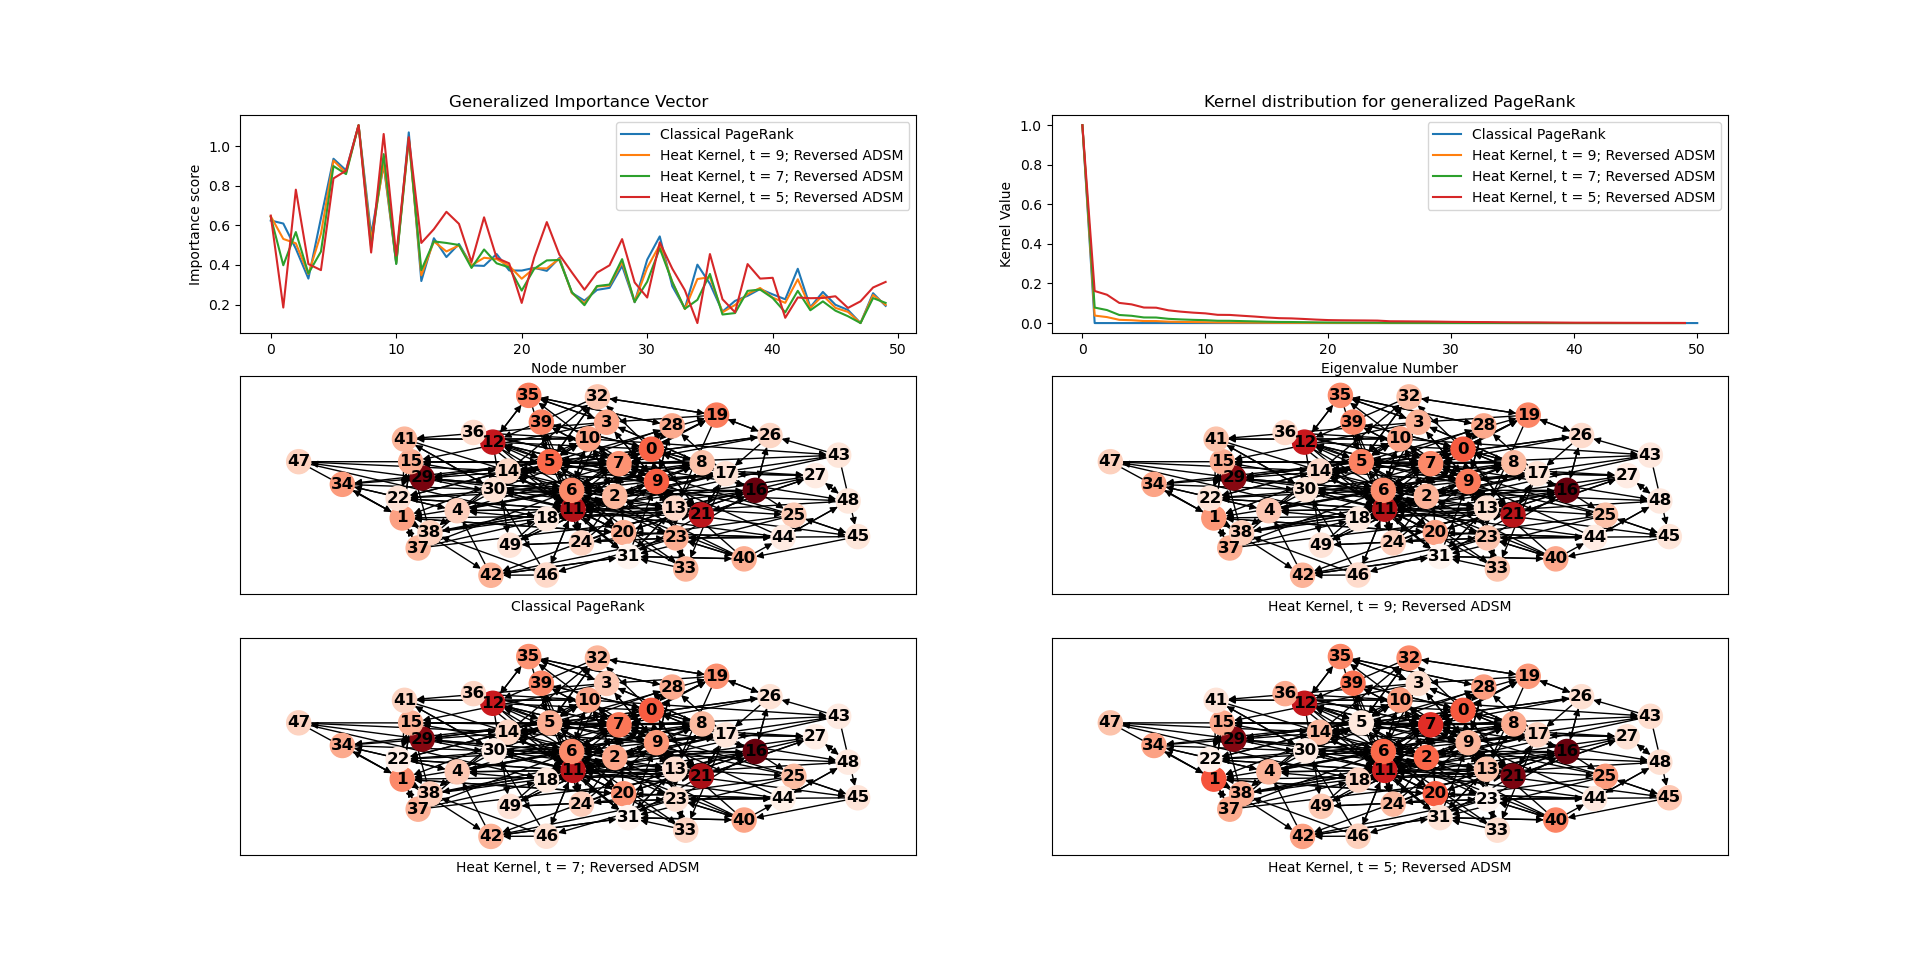
\includegraphics[width= 1.55\textwidth]{results_figures/heat_kernel_comparison.png}
    }
    \caption{Generalized PageRank Simulation Using different heat Kernels for the Reversibilized version of the ADSM}
    \label{fig:heatKComparison}
\end{figure}

\begin{figure}[h!]
    \centering
    \centerline{
    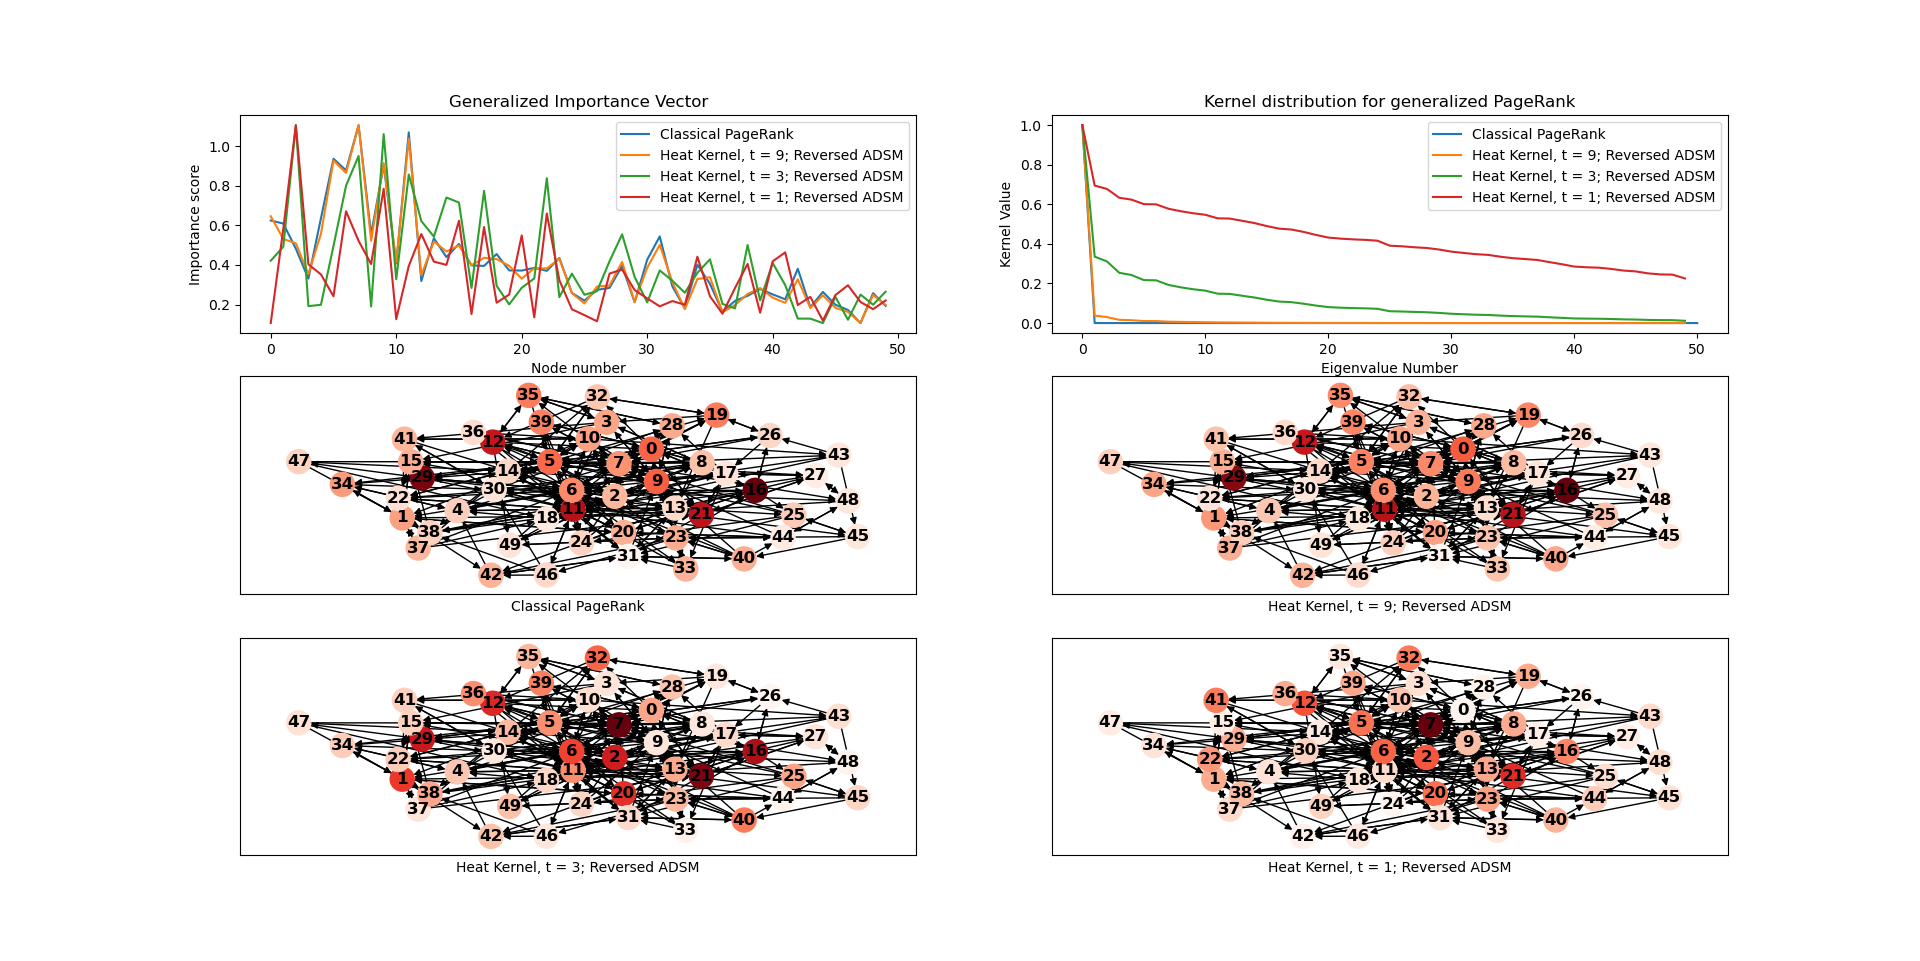
\includegraphics[width= 1.55\textwidth]{results_figures/heat_kernel_comparison_2.png}}
    \caption{Generalized PageRank Simulation Using different heat Kernels for the Reversibilized version of the ADSM}
    \label{fig:heatKComparison2}
\end{figure}

\begin{figure}[h!]
    \centering
    \centerline{
    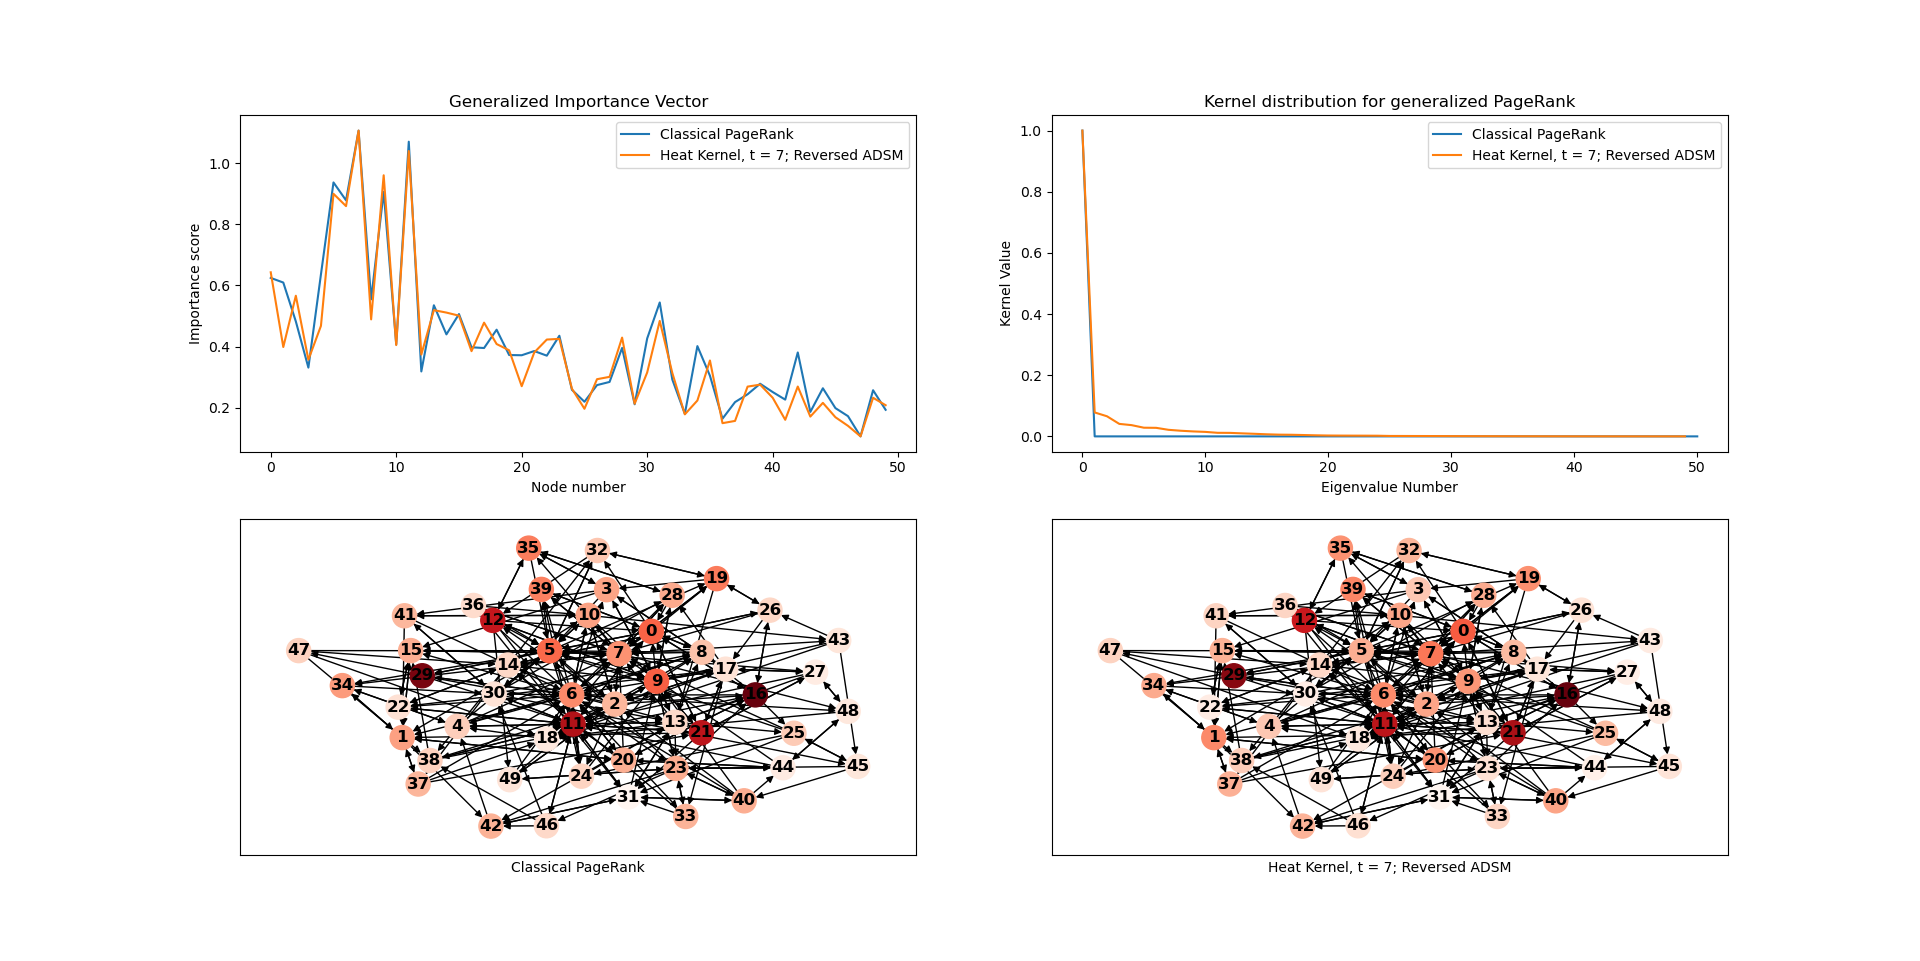
\includegraphics[width= 1.55\textwidth]{results_figures/heat_kernel_7.png}
    }
    \caption{Generalized PageRank heat Kernel comparison with the Classical PageRank. Parameter : time = 7}
    \label{fig:heatK9}
\end{figure}

On the figures \ref{fig:heatK9} \ref{fig:heatK5} and \ref{fig:heatK3}, we compare individually the behaviour of the Generalized Importance Vector to the Classical PageRank for Heat Kernels of parameters $t \in \{9, 5, 3\}$. 

\begin{figure}[h!]
    \centering
    \centerline{
    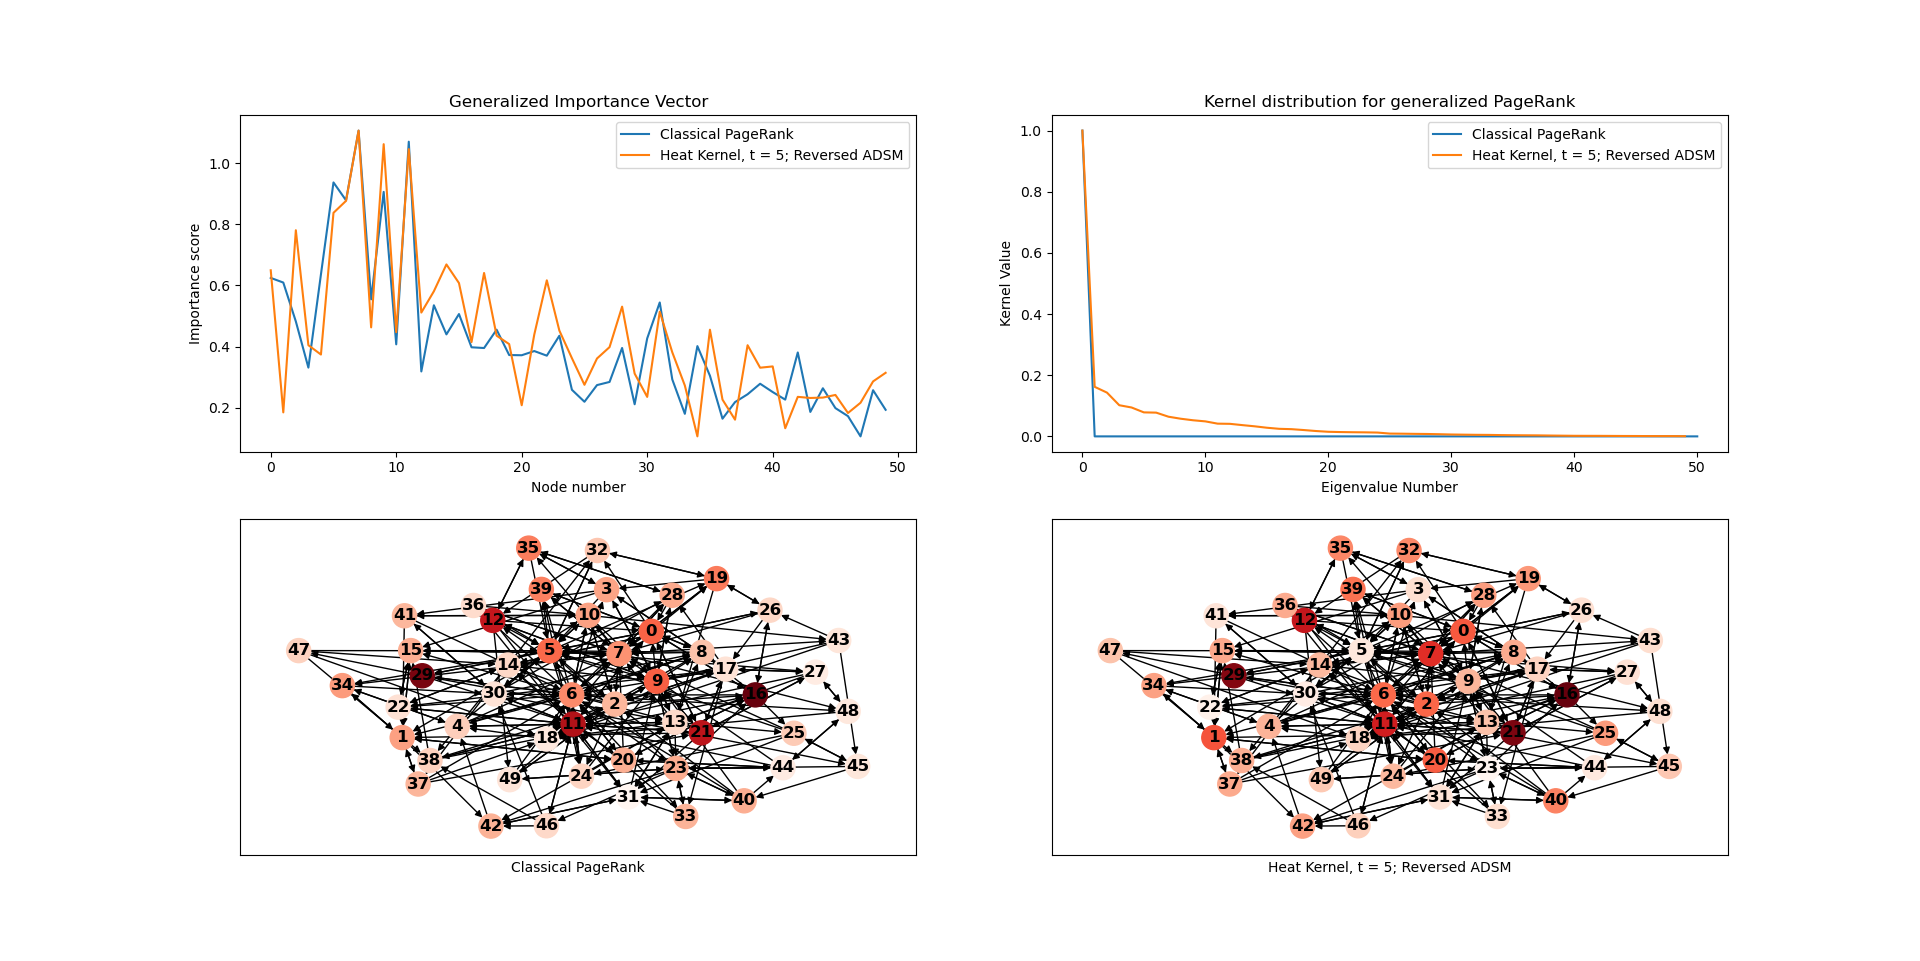
\includegraphics[width= 1.55\textwidth]{results_figures/heat_kernel_5.png}
    }
    \caption{Generalized PageRank heat Kernel comparison with the Classical PageRank. Parameter : time = 5}
    \label{fig:heatK5}
\end{figure}


\begin{figure}[h!]
    \centering
    \centerline{
    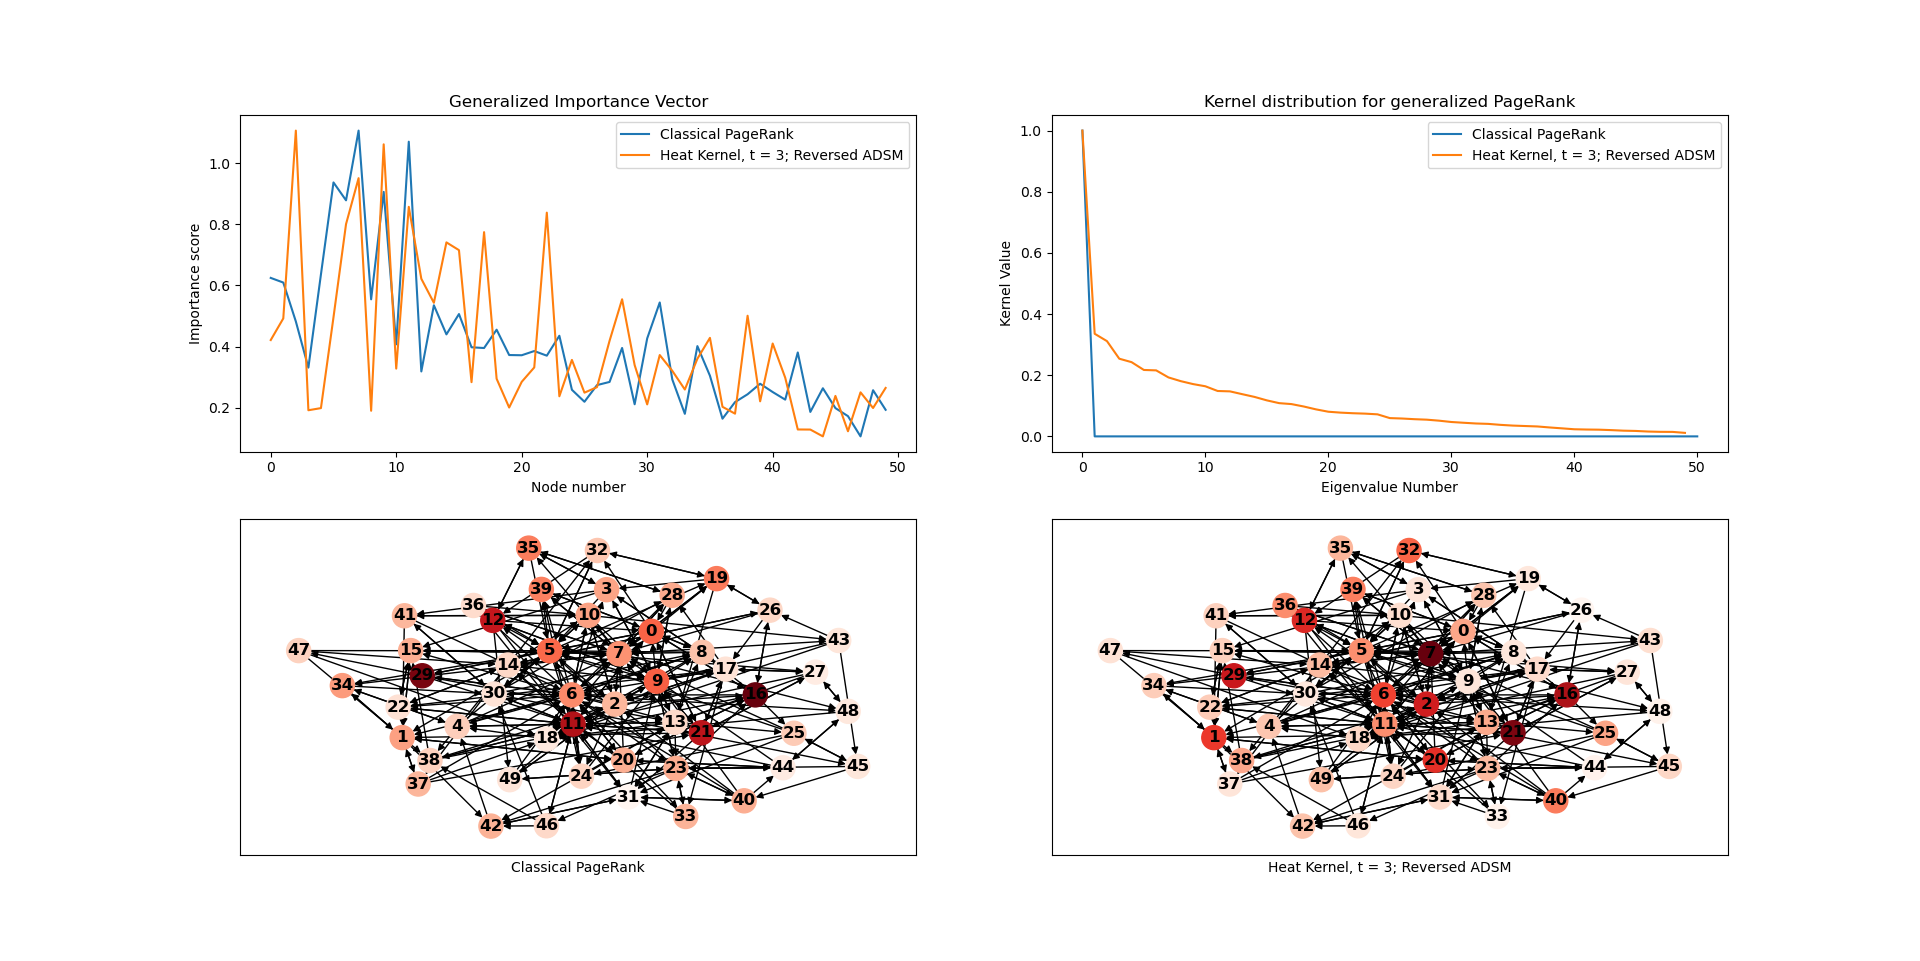
\includegraphics[width= 1.55\textwidth]{results_figures/heat_kernel_3.png}
    }
    \caption{Generalized PageRank heat Kernel comparison with the Classical PageRank. Parameter : time = 3}
    \label{fig:heatK3}
\end{figure}

Several interesting Kernels can be used to prepare less common rankings, we have given some examples of such Kernels in \ref{fig:cosineK3} (cosine Kernel), \ref{fig:monomialK3} (monomial Kernel) and \ref{fig:inverseKcomparison} (inverse Kernel). The monomial Kernel \ref{fig:monomialK3} seems to preserve the most important nodes better than the heat Kernels \ref{fig:heatK3}, while enhancing the secondary hubs. The inverse kernels \ref{fig:inverseKcomparison} seem to converge slower to the stationary distribution while being more sensitive to the exponent parameter. Finally the cosine Kernel \ref{fig:cosineK3}, provides a more equalitarian ranking where secondary hubs achieve score similar to the ones of principal hubs.

Besides, \ref{fig:ranking1} and \ref{fig:ranking2} provide a comparison of the rankings obtained for the classical PageRank and our generalized PageRank for two different Kernels (the classical Google Kernel and the Heat Kernel of parameter 1). One can see that while the Classical Google Kernel outputs a ranking that is fairly similar to the classical Google PageRank, the Heat Kernel outputs a new importance vector, that keeps the first ranked nodes at a high position while giving more importance to nodes coming from secondary hubs.

Finally, \ref{fig:benchmark} provides a first benchmark for convergence analysis of ADSM using the power method. One can note that the number of iterations given a precision epsilon remains constant increasing the number of nodes of randomly generated Barabasi-Albert graphs. Adding this observation to the fact that ADSM are sparse matrices, computing the reversibilized version of an ADSM can be done in $\mathcal{O}(nnz(P))$ operations, which $P$ the transition matrix of the input graph - which is at least as fast as the classical PageRank. 

\begin{figure}[h!]
    \centering
    \centerline{
    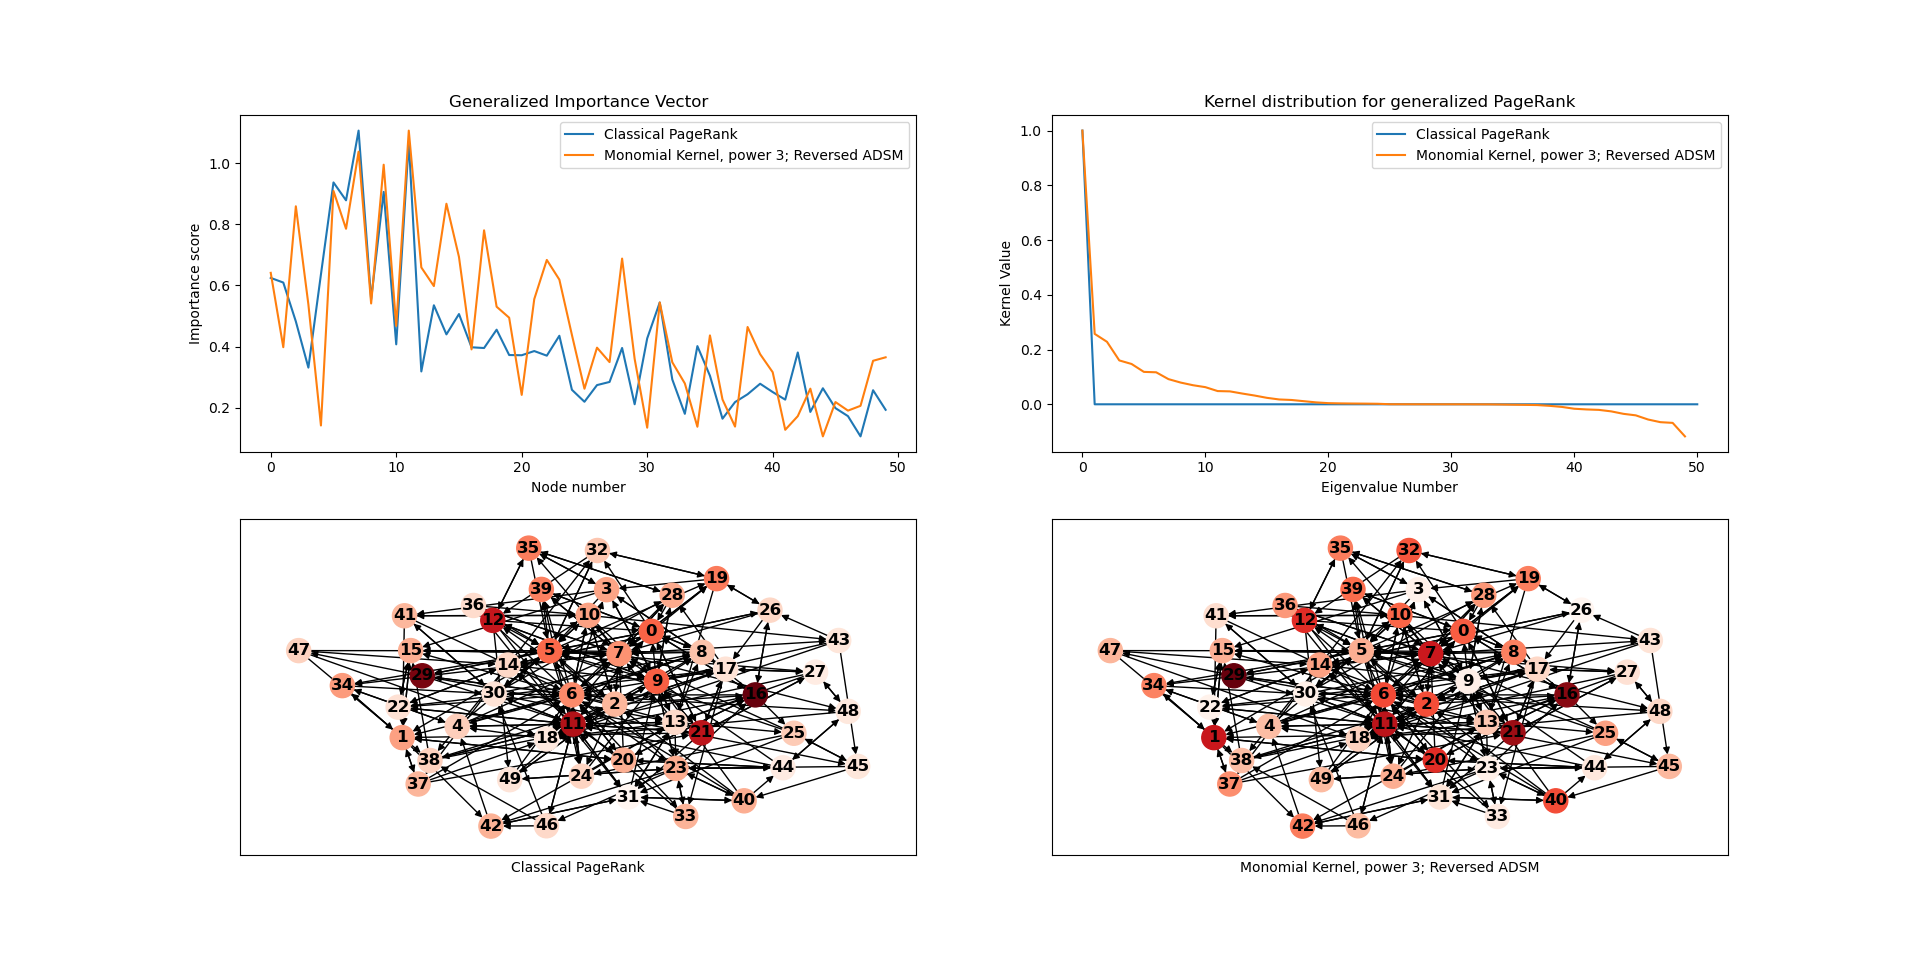
\includegraphics[width= 1.55\textwidth]{results_figures/monomial_kernel_3.png}
    }
    \caption{Generalized PageRank Monomial Kernel comparison with the Classical PageRank. Parameter : exponent = 3}
    \label{fig:monomialK3}
\end{figure}

\begin{figure}[h!]
    \centering
    \centerline{
    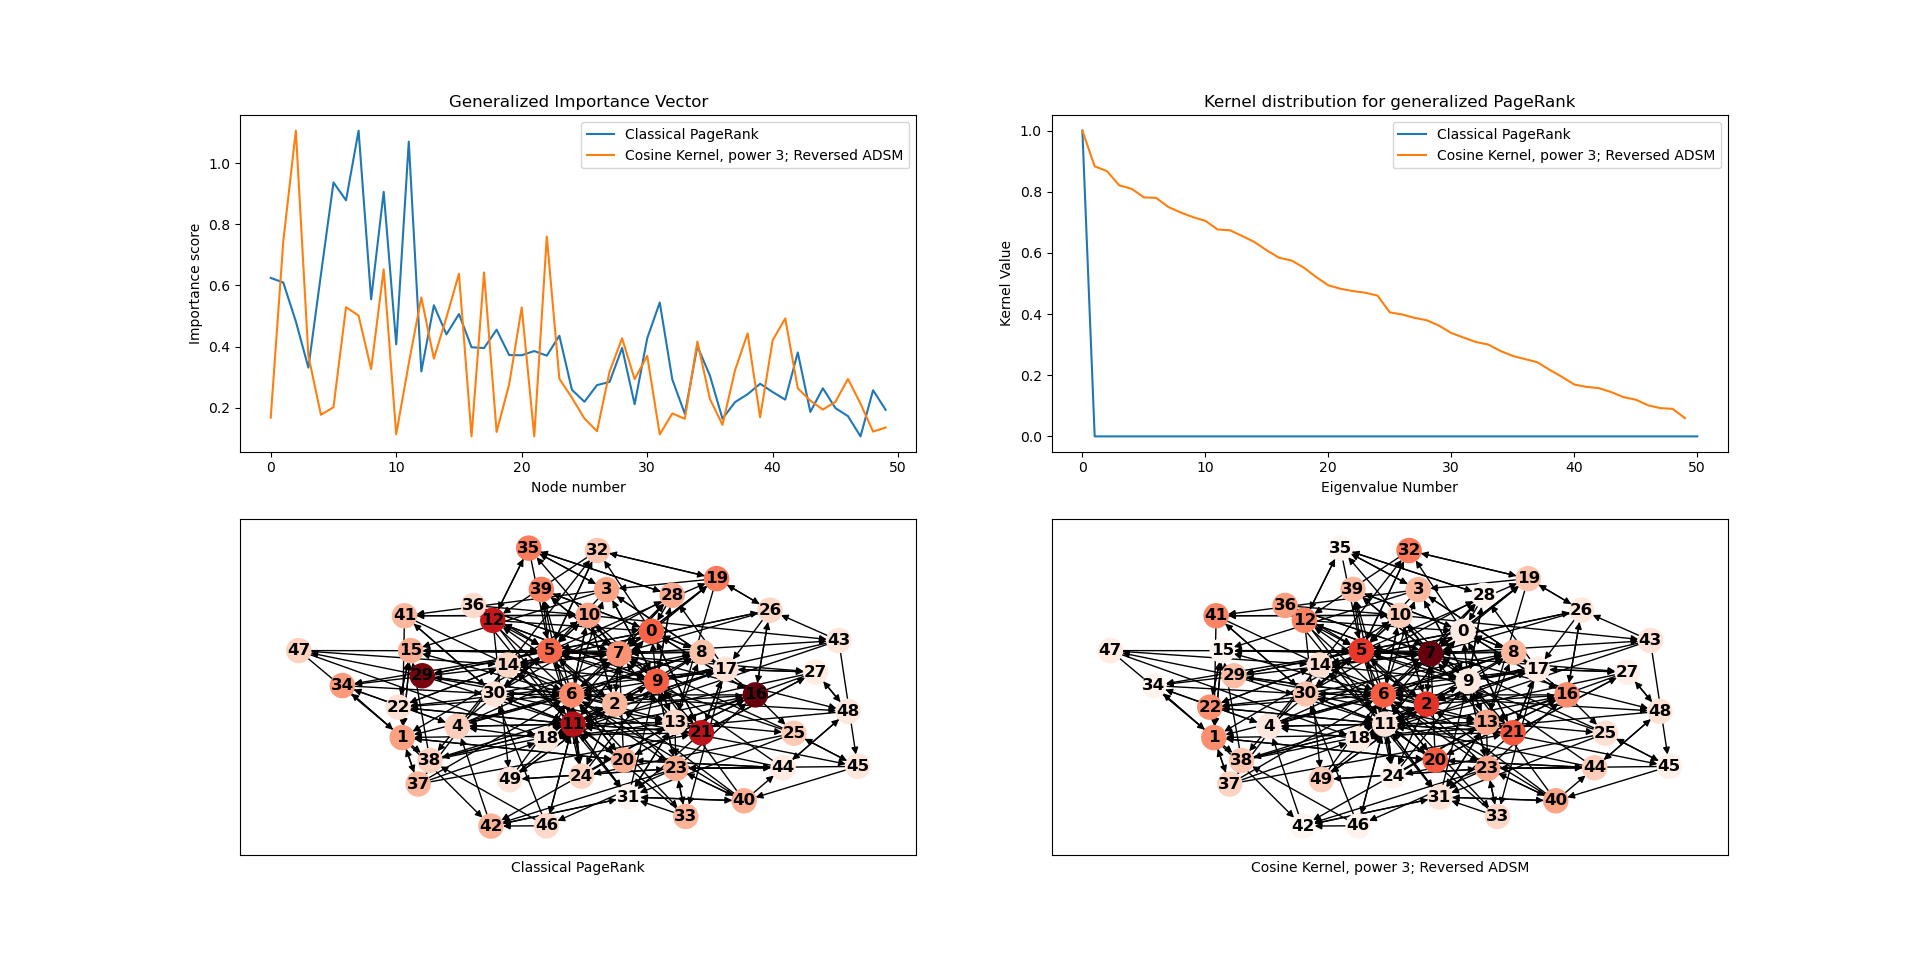
\includegraphics[width= 1.55\textwidth]{results_figures/cosine_kernel_3.png}
    }
    \caption{Generalized PageRank Cosine Kernel comparison with the Classical PageRank. Parameter : exponent = 3}
    \label{fig:cosineK3}
\end{figure}

\begin{figure}[h!]
    \centering
    \centerline{
    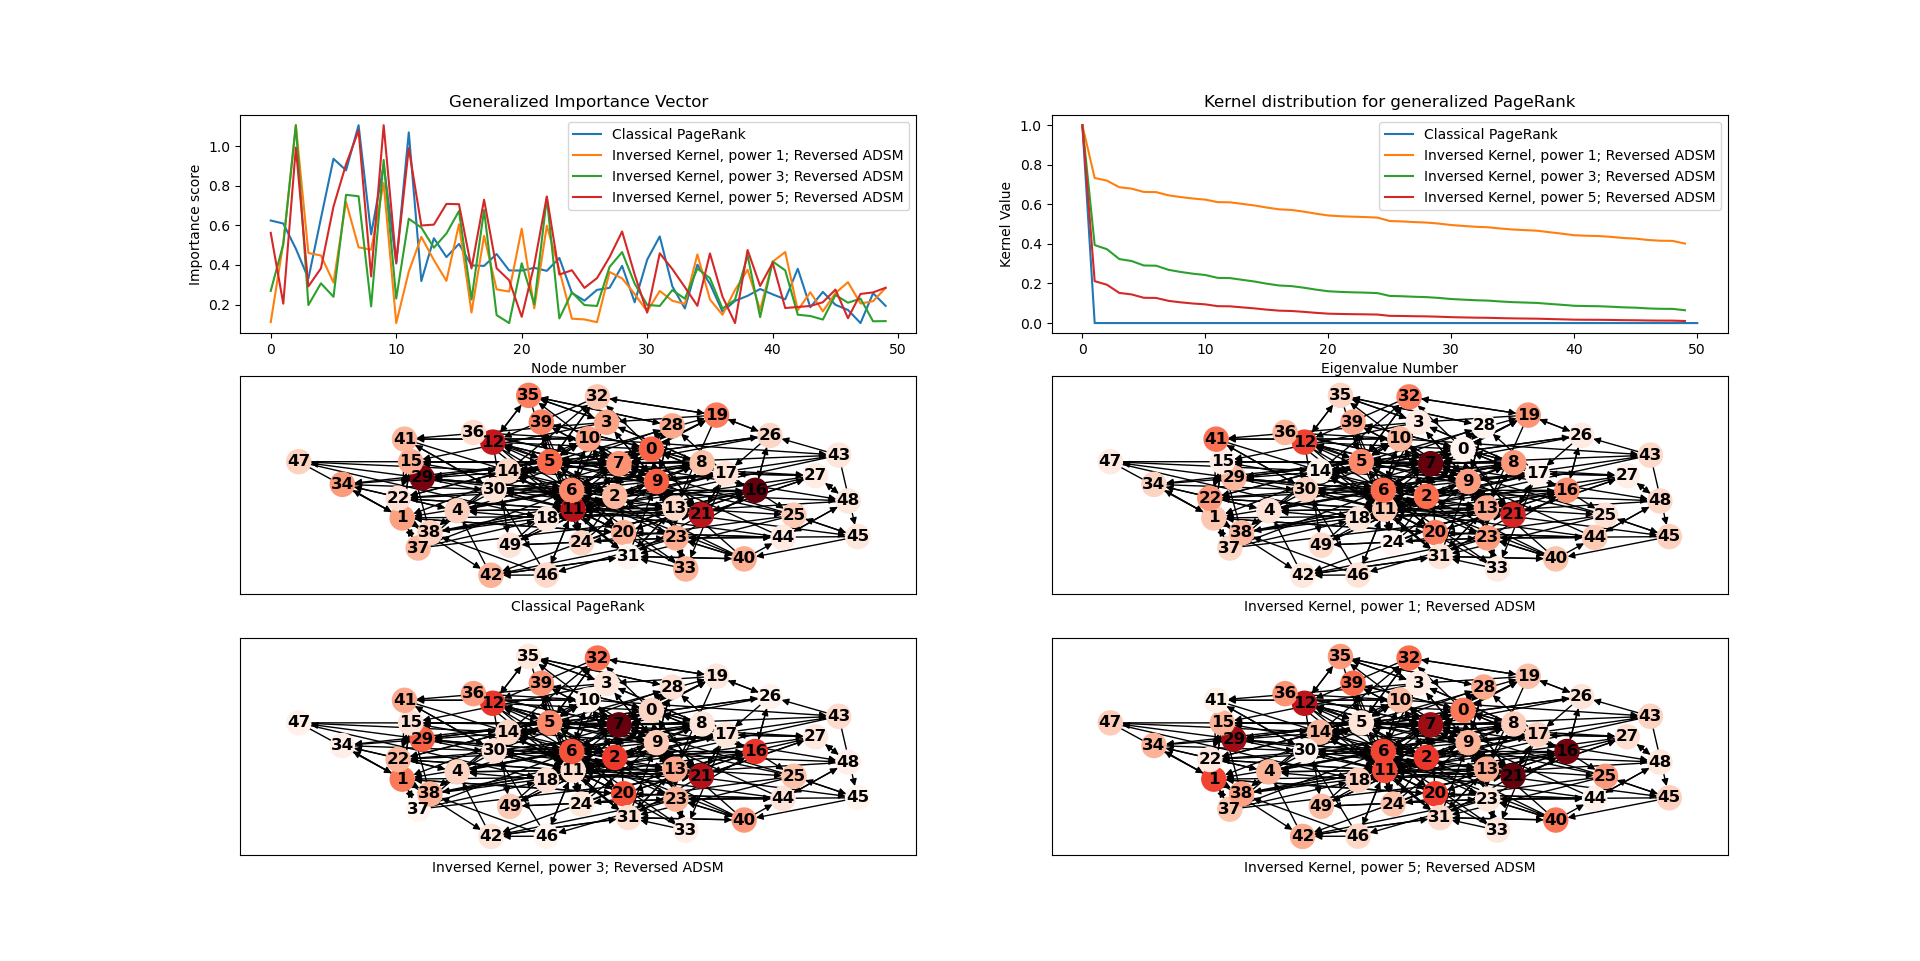
\includegraphics[width= 1.55\textwidth]{results_figures/inverse_kernel_comparison.png}
    }
    \caption{Generalized PageRank Inverse Kernel comparison with the Classical PageRank. Several Parameters}
    \label{fig:inverseKcomparison}
\end{figure}

\begin{figure}[h!]
\centering
\begin{tabular}{c|c|c}
    \textbf{Order} & \textbf{Classical PageRank} & \textbf{Generalized PageRank} \\
    \hline
    1 & 9 & 9 \\
    2 & 10 & 10\\
    3 & 72 & 50\\
    4 & 50 & 72\\
    5 & 48 & 31 \\
    6 & 31 & 71\\
    7 & 71 & 48\\
    \hline
    
\end{tabular}

    \caption{Ranking comparison between the classical Pagerank and the generalized pagerank using the importance vector $(1, 0, \hdots, 0)$}
    \label{fig:ranking1}
\end{figure}



\begin{figure}[h!]
    \centering
    
\begin{tabular}{c|c|c}
    \textbf{Ordre} & \textbf{Classical PageRank} & \textbf{Generalized PageRank} \\
    \hline
        1 & 30 & \textbf{50} \\
    2 & 28 & 32\\
    3 & 68 & 8\\
    4 & 8 & 11\\
    5 & 29 & 40 \\
    6 & 12 & 31\\
    7 & \textbf{50} & 28\\
    \hline
    
\end{tabular}

    \caption{Ranking comparison between the classical Pagerank and the generalized pagerank using the importance vector $(e^{\lambda_0}, e^{\lambda_1}, \hdots, e^{\lambda_n})$, with $\lambda_i$ the $i^{th}$ eigenvalue of the ADSM}
    \label{fig:ranking2}
\end{figure}

\begin{figure}
    \centering
    \begin{tabular}{c|c}
        \textbf{Number of nodes} & \textbf{Number of iterations}\\
        \hline
        100 & 21 \\
        215 & 22 \\
464 & 22 \\
1000 & 22 \\
2154 & 21 \\
4641 & 20 \\
10000 & 20 \\
21544 & 18 \\
46415 & 22 \\
100000 & 17
    \end{tabular}
    \caption{Results of convergence benchmark for the ADSM. Precision $10^{-7}$, graph type : Barabasi-Albert, parameter $5$}
    \label{fig:benchmark}
\end{figure}

\newpage
\section{Second contribution : Quantum Algorithms for Graph Fourier Transform Computation}
\label{sec:quantumPagerank}

\textit{Throughout this section, we will assume given an input directed weighed graph $\mathcal{G}=(V,E,W(E))$ and its associated transition matrix $P$.}

In this section, we introduce a Quantum Algorithms that may be used in application to the theory developed in \ref{sec:SGTapplicationToPR}.
Our method, based on the Quantum Singular Value Transformation introduced by \cite{gilyén_su_low_wiebe_2019}, is used to prepare a quantum state that reproduces a wide range of spectral graph Fourier transforms. The generalized PageRank theory introduced in \ref{sec:SGTapplicationToPR} is derived as at a particular application of our novel algorithm - this first algorithm has indeed a vast range of applications within the SGT.
    
\subsection{Graph Fourier eigenbasis filtering based on Quantum SVT.}

\subsubsection{Elements of Singular Value Transformation}
\paragraph{Singular Value Decomposition:}
Any $n\times m$ matrix admits a Singular Value Decomposition (SVD), ie for every matrix $A \in \mathcal{M}_{n\times m}(\mathbb{K})$, with $\mathbb{K} = \mathbb{R}$ or $\mathbb{C}$, there exists a pair of unitaries $(U,V)\in \mathcal{M}_{n\times n}(\mathbb{K}) \times \mathcal{M}_{m\times m}(\mathbb{K})$, and a diagonal $n \times m$ matrix $\Sigma$ such that (here $\dagger$ is the standard adjoint operator in $\mathbb{R}$ or $\mathbb{C}$):

\begin{equation}
    A = U \Sigma V^\dagger
\end{equation}
The elements of $\Sigma$ are called \textit{Singular Values} of $A$, the columns of $U$ are the \textit{left singular vectors} of $A$ and those of $V$ the \textit{right singular vectors} of A. Besides, if $A$ is real, one can also guarantee $U$ and $V$ to be orthogonal.

The SVD is an extremely popular matrix decomposition that has spread to several fields of Computer Science and Mathematics, such as image compression \cite{image_compression_svd}, signal processing \cite{alter_brown_botstein_2000} and recommender systems \cite{fang_guo_ding_lan_2014}. These numerous applications have made the SVD a well studied and extremely powerful linear algebra tool. 

One first capital result we will extensively exploit in this paper links the SVD to the eigendecomposition :

\begin{propriete}[SVD and eigendecomposition]\label{propriete:svd_eigen}
    Let $A$ be a $n\times m$ real or complex matrix, $(U,V)$ unitaries matrices and $\Sigma$ a diagonal matrix so that $A = U\Sigma V^\dagger$, then :
    \begin{itemize}
        \item The non-zero singular values (diagonal elements of $\Sigma$) are the square roots of the non-zero eigenvalues of $AA^\dagger$ and $A^\dagger A$
        \item The left-singular vectors (columns of $U$) are the eigenvectors of $A^\dagger A$
        \item The right-singular vectors (columns of $U$) are the eigenvectors of $A A^\dagger$
    \end{itemize}
    
    In particular, if $A$ is a square positive semi-definite normal matrix (ie $AA^\dagger = A^\dagger A$ and the eigenvalues of $A$ are non-negative), then the SVD and the eigendecomposition of $A$ are the same.
    
\end{propriete}

\paragraph{Singular Value Transformation:}

In \cite{gilyén_su_low_wiebe_2019}, A. Gilyén et all define the Singular Value Transformation as :

\begin{definition}[Singular Value Transformation]
Let $P \in \mathbb{C}[X]$ be a polynomial and $A$ an operator, whose SVD is $A = W\Sigma V^\dagger$. 

Then the $P$-Singular Value Transformation of $A$ is the transformation:

\begin{equation}
        P^{(SV)}(A) := \left\{ \begin{array}{cc}
            WP(\Sigma)V^\dagger & \mbox{if P is odd} \\
            VP(\Sigma)V^\dagger & \mbox{if P is even}
        \end{array} \right.
\end{equation}

\end{definition}

This former definition of Singular Value Transformation, relies on the notion of \textit{projected unitary encodings}:

\begin{definition}[Projected unitary encodings/Block encodings \cite{gilyén_su_low_wiebe_2019}]

Let $\widetilde{\Pi}$ and $\Pi$ orthogonal projectors, $U$ a unitary and $A$ any real operator, we say that $(\widetilde{\Pi}, \Pi, U)$ form a projected unitary encoding of $A$ iff : 
\begin{equation}
    A = \widetilde{\Pi} U \Pi
\end{equation}

From now on, to avoid confusion with the limit probability distribution $\Pi$, we choose to use the letter $R$ to represent projected unity encodings - modifying the notations used in \cite{gilyén_su_low_wiebe_2019}.

In the next section, we are going to use particular case of Unitary Encoding: Block encodings.

Suppose A is an s-qubit operator, $\alpha, \epsilon \in \mathbb{R}_+$ and $a \in \mathbb{N}$. We say that the $(s+a)-qubit$ unitary U is an $(\alpha, a, \epsilon)$-block encoding of A if :
\begin{equation}
    \|A - \alpha(\bra{0}^{\otimes a} \otimes I) U (\ket{0}^{\otimes a} \otimes I) \| \leq \epsilon
\end{equation}

In other words, the top left block of the matrix $U$ is an $\nicefrac{\epsilon}{\alpha}$-close approximation of $\nicefrac{A}{\alpha}$.

\end{definition}

These projected unitary encoding are used to make the bridge between Quantum unitary operators ($U$) and classical operators ($A$). In fact, if $(\widetilde{R}, R, U)$ forms a projected unitary encoding of $A$, quantum circuits will act on the operator $U$ whose changes will reflect the Singular Value Transformation on $A$ via the orthogonal projections $\widetilde{R}$ and $R$. In other words, given a degree-d odd polynomial, bounded by 1 in absolute value on [-1, 1], the singular value transformation performs the operation :

\begin{equation}
    A = \widetilde{R} U R \rightarrow P^{SV}(A) = \widetilde{R} U_{\phi} R
\end{equation}

Where the unitary $U_\phi$ can be implemented with a circuit using $U$ and its inverse $d$ times. In the case where $P$ is even, the same result holds, replacing $\widetilde{R}$ by $R$.

These results are considerably powerful, as the authors of \cite{gilyén_su_low_wiebe_2019} manage to derive a several use cases of their Quantum Singular Value Transformation while featuring near optimal complexity for every algorithm. Application fields include Quantum Walks, Matrix Arithmetics, Quantum Machine Learning and Quantum Language theory. Our paper will prove that Singular Value Transformation provides an powerful framework to implement a wide range of inverse graph Fourier Transforms, being on the very first Quantum based Spectral Graph Theory algorithms of this kind. As a direct application, we will show how to derive a Quantum Graph Fourier Transform based PageRank algorithm, exploiting the results presented in \ref{sec:SGTapplicationToPR}.

\subsubsection{On Graph Frequency-Based inverse Fourier Transform}

Our algorithm is able to solve the following problem :

\paragraph{Input:}\label{par:algo_1_inputs} Let $C$ be a regular, reversible Markov Chain on the Graph $\mathcal{G}$ with transition matrix $P$ and let $(u_1, \hdots, u_n)$ be its Fourier Basis associated with eigenvalues $(\lambda_1, \hdots, \lambda_n)$. Let $h: \mathbb{R} \rightarrow \mathbb{R} $ a real sequentially continuous function. For every $\epsilon > 0$, $h$ admits an $\epsilon$-close Polynomial approximation by a polynomial $Q$ of degree $d(\epsilon)$, such that $\forall x \in [-1,1], \|Q(x)\|< \nicefrac{1}{2}$. Let $h(\lambda_i)_{i\in [1, n]}$ a graph Kernel defined by : $h(\lambda_i)_{i\in [1, n]}=(h(\lambda_1), \hdots, h(\lambda_n))$

\paragraph{Output:} A Quantum state $\ket{\psi_o}$ representing the inverse graph Fourier transform of $h(\lambda_i)_{i\in [1, n]}$, as defined in \ref{def:directed_graph_fourier_transform} :

\begin{equation}
    \ket{\psi_o} = \sum_{i \in [1,n]} \Tilde{h}(\lambda_i) \ket{u_i} 
\end{equation}

Where $\|\Tilde{h} - h\|_{[0,1]} < \epsilon$.

Hence, from this formulation, and the definition \ref{def:generalized_importance_vector} one can understand that this problem is tightly related to our generalized PageRank framework.

These methods suppose granted an efficient access to a Quantum memory (QRAM for instance) being able to represent Classical data in a quantum state.\label{rmq:QRAM_assumptions} \cite{giovannetti_lloyd_maccone_2008} introduced a bucket brigade QRAM structure which may be able to provide and store classical information in $\mathcal{O}(poly-log(n))$ complexity. However, this structure does not seem to provide a sufficient enough stability to guarantee constant error prediction for sublinear complexity Quantum based algorithms (see \cite{arunachalam_gheorghiu_jochym-o’connor_mosca_srinivasan_2015} for more detailed explanations). Other data structures were introduced since the Bucket Brigade version, see \cite{park_petruccione_rhee_2019} for instance. 

Besides, the complexity results depend heavily on the regularity of the function $h$. Indeed, the algorithm time complexity depends directly on the degree of a polynomial approximation of $h$. We are proposing a detailed analysis of the complexity of the Quantum algorithm in \ref{subsubsec:algo_1_complexity}.

\subsubsection{Quantum SVT major steps.}
Here are the major steps of our Graph Fourier Transform computation method. We are given a regular and reversible transition matrix $P$, and define $\mathcal{P} := \Pi^{-1/2} P \Pi^{1/2}$, where $\Pi$ is the probability limit distribution of $P$. $\mathcal{P}$ is decomposed as $\mathcal{P}= U \Sigma U^T$ using SVD : indeed, since $P$ is regular, $\mathcal{P}$ is symmetric and the SVD of $\mathcal{P}$ is exactly its eigendecomposition. \\

\textbf{Step 1 :} - We suppose being given $2b = 2 log_2(N)$ initial QBits in the state $\ket{0}_A \ket{0}_B$, such as the register $A$ and the register $B$ contains both exactly $b$ qBits. Prepare the initial Quantum state $\ket{\psi_P}=\sum \mathcal{P}_{i,j} \ket{i}_A \ket{j}_B = \sum_{k=1}^T \sigma_k \ket{u_k}_A \ket{v_k}_B$, the same way as \cite{lin_bao_zhang_li_wang_2019} and \cite{duan_yuan_liu_li_2018}. The preparation of this initial state can be performed by using a QRAM where one can retrieve the values of $\mathcal{P}_{i,j}$ for state preparation.\\

\textbf{Step 2 :} - Let $(\bra{0} \otimes Id, \ket{0} \otimes Id, U) $ be a unitary encoding of $\mathcal{P}$ such that $(\ket{0}\bra{0} \otimes Id) U (\ket{0}\bra{0} \otimes Id) = \begin{pmatrix} \mathcal{P} & 0 \\ 0 & 0 \end{pmatrix}$. This step consists in combining the results of \cite{gilyén_su_low_wiebe_2019} to get build circuits that can produce the polynomial transformations $T_i^{SV}(\mathcal{P}) = \widetilde{R} U_{\phi_i} R$. Then, one can use the block matrix arithmetic results (Lemma 53 of \cite{gilyén_su_low_wiebe_2019}) to build successions of block encoding unitaries - since $T(\mathcal{P}) = U T(\sigma) U^T$, applying two successive polynomials $T_1$ and $T_2$ to $\mathcal{P}$ amounts to applying directly the product $T_1 \times T_2$ to $\mathcal{P}$. Here one only need to use the product of two block encoding unitaries: the first one encoding a polynomial approximation of the inverse function on [-1,1], the second one encoding any polynomial Q of degree d bounded by $1/2$.

\begin{itemize}
    \item \textbf{First unitary: Inverse function approximation}. Since the matrix $\mathcal{P}$ is invertible, there exist a $\delta>0$ such that $\forall x \in [-\delta, \delta], x \not\in Sp(\mathcal{P})$ where $Sp(\mathcal{P})$ is the spectrum of $\mathcal{P}$. Then, according to the \textit{Corollary 69} of \cite{gilyén_su_low_wiebe_2019}, there is an odd polynomial $L \in \mathcal{R}[X]$ of degree $\mathcal{O}(\nicefrac{1}{\delta} log(\nicefrac{1}{\epsilon})$ that is $\epsilon-approximating$ the function $f(x) = \frac{3\delta}{4 x}$ on the domain $I = [-1, 1] \setminus [-\delta, \delta]$. \cite{gilyén_su_low_wiebe_2019} gives a method to build recursively the polynomial $P$. Then using Quantum Singular Value Transformation, one can build the operator $U_{\phi}$ so that $(\ket{0}\bra{0} \otimes I)U_{\phi}(\ket{0}\bra{0} \otimes I) = \begin{pmatrix} L^{(SV)}(\mathcal{P}) & 0 \\ 0 & 0 \end{pmatrix}$
    \item \textbf{Second unitary : h function approximation}. We apply Hermitian Quantum Singular Value Transformation (Theorem 56) from \cite{gilyén_su_low_wiebe_2019} to build the operator $U_{\phi}$ so that $(\ket{0}\bra{0} \otimes I)U_\phi (\ket{0}\bra{0} \otimes I) = \begin{pmatrix} Q^{(SV)}(\mathcal{P}) & 0 \\ 0 & 0 \end{pmatrix}$. 
    
    \item \textbf{Patching up : Multiplication of the previous encodings.} The multiplication theorem of \cite{gilyén_su_low_wiebe_2019} provides a final unitary encoding of $T(\mathcal{P}) L(\mathcal{P})$ : $\widehat{U}$.
    
\end{itemize}

\textbf{Step 3:} - Apply $\widetilde{R}\widehat{U} R$ to the register B. The system state is now $\ket{\psi_3} = \sum_i Q(\lambda_i) \ket{u_i}\ket{u_i}$.\\

\textbf{Step 4:} - Uncompute the register B. This can be done without the need of external ancilla qBits, by only applying CNOT gates to every pair of QBits from register A and B. After the operation, the register B will be in the pure state $\ket{0}_B$ and one can uncompute it by measurement.\\

\textbf{Step 5 :} The final system state is $\ket{\psi_f} = \sum_i Q(\lambda_i) \ket{u_i}$.

\subsubsection{Detailed explanation of the main steps of the algorithm.}\label{subsubsec:algo_1_explanation}

This algorithm relies on the property \ref{propriete:svd_eigen} : for normal semi-definite matrices the eigendecomposition and SVD coincides. Hence, reversible transition matrices $P$ being adjoint operators in the space $l^2(V, \pi)$, the operator $\mathcal{P} = \Pi^{-1/2} P \Pi^{1/2}$ is an adjoint operator in the classical $l^2(V)$ space, equipped with the standard inner product - ie $\mathcal{P}^* = \mathcal{P}^T = \mathcal{P}$ (see remark \ref{subsec:vector_spaces_relation}. The whole framework developed in \ref{sec:SGTIntro} then directly applies to the SVD of $\mathcal{P}$, which explains how one can simply identify the singular values to eigenvalues and eigenvectors to singular vectors for the matrix $\mathcal{P}$.\\
Our algorithm also applies to non reversible transition matrices, however one looses some properties introduced in \ref{sec:SGTIntro}: we discuss the non reversible case in \ref{subsubsec:algo_1_extensions}.

For \textbf{Step 2}, the polynomial $T$ can represent a wide range of functions. We are going to give several examples of Kernel functions $h$ in \ref{subsubsec:algo_1_extensions}.  

In our SVT algorithm, we build explicitly a unitary encoding $(\mathcal{R}, R, U)$ of $\mathcal{P}$, drawing our inspiration from \cite{gilyén_su_low_wiebe_2019} construction used in its \textit{Corollary 34}, which stems from Szegedy's construction of Quantum Walk Operators (see \ref{subsubsection:Paparo_quantum_walk}). Indeed, the unitary $U = U_L^\dagger U_R$ is formed thanks to the two state preparation unitaries $U_L$ and $U_R$:

\begin{align}
    U_R : \ket{0} \ket{x} &\rightarrow \sum_{y \in V} \sqrt{P_{xy}} \ket{x} \ket{y} \\
    U_L : \ket{0} \ket{y} &\rightarrow \sum_{x \in V} \sqrt{P^*_{yx}} \ket{x} \ket{y}
\end{align}

Which implies, choosing $R = \widetilde{R} = (\ket{0}\bra{0} \otimes I)$, that $\widetilde{R}UR = \begin{pmatrix} \mathcal{P} & 0 \\ 0 & * \end{pmatrix}$. Indeed, we remind that $P^*_{x,y} := P_{y,x} \frac{\pi(y)}{\pi(x)}$, which allows getting $\mathcal{P}$ from $(\sqrt{P_{xy}P^*_{yx}})_{ij \in [1,n]}$.

Using the above operator, and apply it to the register B and a b-size ancilla set of qBits, yields :

\begin{align}
    \sum_{k\in [1,n]} \sigma_k \ket{u_k}_A \widetilde{R}U_\phi R (\ket{v_k}_B \ket{0}_C) &= \sum_{k\in [1,n]} \sigma_k \ket{u_k}_A  (\sum_{i \in [1,n]} T(\sigma_i) \ket{u_i}\bra{v_i}\ket{v_k}_B) \ket{\zeta}_C )\\
    &= \sum_{k\in [1,n]} \sigma_k T(\sigma_k) \ket{u_k}_A  \ket{u_k}_B \ket{\zeta}_C \\
    &= \sum_{k\in [1,n]} Q(\sigma_k) \ket{u_k}_A  \ket{u_k}_B \ket{\zeta}_C \\
    &= \sum_{k\in [1,n]} Q(\sigma_k) \ket{u_k}_A  \ket{u_k}_B
\end{align}

Let's simply recall that the $\ket{v_i}$ form an orthonormal basis of vectors, which allows one to derive the second line equality in the previous set of equations.

The register C being untangled from register B, due to the diagonal block-form of the operator $\widetilde{R}U_\phi R$, one can uncompute the register without modifying the global state of the system.

\paragraph{Circuit implementation of the algorithm:}
The figure \ref{fig:quantum_circuit_algo_1} presents a macroscopic Quantum Circuit implementation of the algorithm introduced in the previous paragraph. 
\begin{figure}
    \centering
    $\begin{array}{c}
    \Qcircuit {
    \lstick{C : \ket{0}_{n_b}} & {/} \qw &\qw &  \multigate{1}{\widetilde{R}U_\phi R} & \meter & \qw & \qw \\
    \lstick{B : \ket{0}_{n_b}} & {/} \qw & \multigate{1}{QRAM}  & \ghost{\widetilde{R}U_\phi R} &  \targ & \meter & \rstick{\ket{0}} \cw \\
    \lstick{A : \ket{0}_{n_b}} & {/} \qw & \ghost{QRAM} & \qw  & \ctrl{-1} &   \rstick{\sum_i \Tilde{h}(\lambda_i) \ket{u_i}} \qw \\
    & & \dstick{\ket{0}_A\ket{0}_B \rightarrow \sum_{ij} P_{i,j} \ket{i}_A \ket{j}_B} \cwx & & & }       
    \end{array}$
    
    \bigskip
    \caption{The Quantum Circuit used by the Graph Fourier eigenbasis filtering}
    \label{fig:quantum_circuit_algo_1}
\end{figure}

\subsubsection{Complexity analysis.}\label{subsubsec:algo_1_complexity}

This algorithm being the combination of three macroscopic quantum processes, one has to estimate the gate and memory cost of each process and sum each individual computational cost to get the global computational cost.

\paragraph{Cost of QRAM state preparation:}
As noticed in \ref{rmq:QRAM_assumptions}, several authors have introduced Quantum Random Access Memory structures that are able to prepare any loaded state in time $\mathcal{O}(polylog(n))$ with a low degree of polynomial scaling. 

\paragraph{Cost of $\widetilde{R}U_\phi R$ preparation:}
Let $(\widetilde{R}, R, U)$ be a unitary encoding of $P$, a real operator. According to the results of \cite{gilyén_su_low_wiebe_2019} (\textit{Corollary 18 
\& Lemma 19}), given a real odd polynomial of degree $d$, bounded by 1 in $[0,1]$, one can build $U_\phi$ - after $\mathcal{O}(poly(d, log(\frac{1}{\epsilon})))$ preprocessing computations on classical computer - using for d-times : 
\begin{itemize}
    \item The operators $U$ and $U^\dagger$
    \item The gates $C_R NOT$ and $C_{\widetilde{R}} NOT$
    \item Single QBit Gates.
\end{itemize}
And uses a constant number of ancila qBits. Which makes the overall number of gates required scaling as $\mathcal{O}(d \mathcal{T}(U))$ with $\mathcal{T}(U)$ the cost of implementing $C_R NOT$ and $U$ gates \cite{gilyén_su_low_wiebe_2019}.

\paragraph{Cost of last $C_{NOT}$ preparation}

The last $CNOT$ operator requires the use of $n_b$ 2-QBits CNOT, which makes an overall of $\mathcal{O}(log(n))$ Quantum gates.

\paragraph{Patching up:}
By combining all the previous equalities, one can deduce that the overall Quantum gate cost to implement the circuit \ref{fig:quantum_circuit_algo_1} scales as $\mathcal{O}(d \mathcal{T}(U) + S(log(n)))$ with $S$ a low degree polynomial. This result proves a direct dependency between the number of quantum gates required and the degree of the polynomial simulated : which explains why our algorithm is most efficient mostly Fourier Kernels well approximated by low degree polynomials.

\subsection{Algorithm Discussions}\label{subsubsec:algo_1_extensions}

We have been able to derive several interesting and general results from a precise exploitation of the Quantum Singular Value Transformation algorithm introduced by A. Gilyén et all \cite{gilyén_su_low_wiebe_2019}. In this part we analyse several extensions to this algorithm that may be of interest, while giving examples of Kernels efficiently implemented within the algorithm.

\paragraph{Undirected graph version:}
Even though until now we have only worked with directed graphs, our Quantum Graph Frequency-Based Inverse Fourier Transform transposes well to the undirected framework. Indeed, undirected graphs are always reversible and symmetric which means that the reversible condition on the input may be dropped in the undirected setting. Several spectral graph theory applications only make use of undirected graphs \cite{ortega_frossard_kovacevic_moura_vandergheynst_2018, shuman_narang_frossard_ortega_vandergheynst_2013, ricaud_borgnat_tremblay_gonçalves_vandergheynst_2019} and our algorithm may be of great use in those cases. Please note also that these undirected graphs does not need to be regular and that our results also apply to undirected non-regular graphs (whereas power method for PageRank does not converge for these graphs).

\paragraph{Non reversible graphs:}
Please also note that our algorithm does produce results for regular non-reversible graphs: however, one looses the direct correspondence between transition matrix singular values and eigenvalues due to the absence of symmetries for the transition matrix. Indeed, the operator $\mathcal{P} = \Pi^{-1/2} P \Pi^{1/2}$ is no longer self-adjoint and one can only claim that the singular values of $\mathcal{P}$ are the square root of the eigenvalues of $\mathcal{P}\mathcal{P}^* = \Pi^{-1/2} P \Pi P^* \Pi^{-1/2}$ which may not yield a simple nor intuitive Spectral Graph based interpretation of eigenspaces.

However, please note that, with several modifications to the original algorithm, one can apply a singular value transformation on a Fourier basis that corresponds to a rescaled version of the original transition matrix P. The following changes have to be performed :

\begin{itemize}
    \item Let $\sqrt{P}$ be the transition matrix such as $(\sqrt{P}_{ij}) = \frac{\sqrt{P_{ij}}}{\sum_{k \in [1,n]} \sqrt{P_{ik}}}$
    
    \item Let $\widehat{\sqrt{P}} = (diag(\frac{1}{\|\sqrt{P}\|_1})^{1/2}) \sqrt{P}$, where :
    \begin{equation}
        diag(\frac{1}{\|\sqrt{P}\|_1})^{1/2} = diag(\sqrt{\frac{1}{\sum_{i\leq n}\frac{\sqrt{P_{i1}}}{\sum_{k \in [1,n]} \sqrt{P_{ik}}}}}, \hdots, \sqrt{\frac{1}{\sum_{i\leq n}\frac{\sqrt{P_{in}}}{\sum_{k \in [1,n]} \sqrt{P_{ik}}}}}
    \end{equation}.
    
    \item Instead of loading the state $\sum_{ij} \mathcal{P}_{ij} \ket{i}_A \ket{j}_B$ from the QRAM, one loads the state $\sum_{ij} \widehat{\sqrt{P}}_{ij} \ket{i}_A \ket{j}_B$ from the QRAM.
    
    \item Instead of preparing the unitaries $U_R$ and $U_L$ in \textbf{Step 2} of our algorithm, one has to prepare the unitaries :
    
    \begin{align}
        \sqrt{U_R} : \ket{0}\ket{x} &\rightarrow \sum_{y\in V} \sqrt{\sqrt{P}_{x,y}} \ket{x} \ket{y} \\
        \sqrt{U_L} : \ket{0}\ket{y} &\rightarrow \sum_{x\in V} \sqrt{\sqrt{P}^{T_{stoch}}_{y,x}} \ket{x} \ket{y}
    \end{align}
    Where the stochastic transposition operator have already been introduced in \ref{def:ADSM1}.
\end{itemize}

The remaining parts of the algorithm remains unchanged. At the issue of the algorithm, one computes the Singular Value Transformation of $\widehat{\sqrt{P}}$, putting the system in the final state $\ket{\psi}_f = \sum_i h(\widehat{\sigma_i}) \ket{\widehat{u_i}}$, where $\widehat{\sigma_i}$ and $\widehat{u_i}$ are respectively the singular values and the singular vectors of $\widehat{\sqrt{P}}$. However, the singular spaces of $\widehat{\sqrt{P}}$ matches the eigenspaces of the matrix :

\begin{equation}
    \widehat{\sqrt{P}}\widehat{\sqrt{P}}^* = (diag(\frac{1}{\|\sqrt{P}\|_1})^{1/2} \times diag(\frac{1}{\|\sqrt{P}\|_0})^{1/2}) \times P \times (diag(\frac{1}{\|\sqrt{P}\|_0})^{1/2} \times diag(\frac{1}{\|\sqrt{P}\|_1})^{1/2})
\end{equation}

Where $diag(\frac{1}{\|\sqrt{P}\|_0})^{1/2} = diag(\frac{1}{\sum_{k\in [1,n]} \sqrt{P_{1k}}}, \hdots, \frac{1}{\sum_{k\in [1,n]} \sqrt{P_{nk}}})^{1/2}$. 

This last matrix is itself similar to the matrix $(diag(\frac{1}{\|\sqrt{P}\|_1})) \times diag(\frac{1}{\|\sqrt{P}\|_0})) P$ which is a rescaled version of $P$.

Thus, the squared singular values of $\widehat{\sqrt{P}}$ are in fact, the eigenvalues of $(diag(\frac{1}{\|\sqrt{P}\|_1})) \times diag(\frac{1}{\|\sqrt{P}\|_0})) P$. The singular vectors of $\widehat{\sqrt{P}}$ are the eigenvectors of $(diag(\frac{1}{\|\sqrt{P}\|_1})^{1/2} \times diag(\frac{1}{\|\sqrt{P}\|_0})^{1/2}) \times P \times (diag(\frac{1}{\|\sqrt{P}\|_0})^{1/2} \times diag(\frac{1}{\|\sqrt{P}\|_1})^{1/2})$.

Please note that while one has lost a direct correspondance between singular values and eigenvalues, one now has a way to compute a wider class of admissible filters. Indeed, now, using the relation $\widehat{\sigma_i}^2 = \widehat{\lambda_i}$, one can compute an approximation of any analytic function $h(x)=\sum_i \gamma_i x^i$ where $sup_{[0,1]} \frac{h(x)}{x} < 1$ and $h(0)=0$ : the even-parity constraint on the polynomial approximation of $h$ have been removed and one can apply the algorithm under the reversible case conditions.

\paragraph{Spectral Graph signal filtering application:}
Another interesting use case of the previous algorithm rises for a slightly modified version of our original problem. Given $\mathcal{P} = \Pi^{-1/2} P \Pi^{1/2}$, where $P$ is a regular and reversible transition matrix, and granted that one can produce an initial quantum superposition of eigenvectors $\ket{u_k}$ of $\mathcal{P}$, $\ket{\psi}_i = \sum_k c_k \ket{u_k}$, for every polynomial $Q$ bounded by 1 on $[-1,1]$, the algorithm presented above can output the state :

\begin{equation}
    \ket{\psi}_f = \sum_k c_k Q(\lambda_k) \ket{u_k} 
\end{equation}
    
Where $\lambda_k$ is the eigenvalue associated with $\ket{u_k}$.

Thus, if $h$ is an analytical function bounded by 1 on $[-1,1]$ $\epsilon$-approximated by a polynomial $Q_\epsilon$ on $[-1,1]$, one can build the state to a precision $\epsilon$ on the values of $h(\lambda_k)$ :

\begin{equation}
    \ket{\psi}_f = \sum_k c_k h(\lambda_k) \ket{u_k} 
\end{equation}

Please note that results can be derived for complex graph filters (according to the corollary 8 of \cite{gilyén_su_low_wiebe_2019}), providing that the norm of the graph filter is bounded by $\nicefrac{1}{4}$ on $[-1,1]$

Another consequence of our last comment is that, given any initial graph signal $\phi$ (which can be written as a quantum superposition of $\mathcal{P}$ Fourier Basis eigenvectors), one can apply the linear filter $h(\lambda_1, \hdots, \lambda_n)$ to its Graph Fourier components, where $h$ is any real function, $\epsilon$-approximated by a given family of polynomials, and bounded by 1 on $[-1,1]$.

Signal filtering is ubiquitous in spectral graph theory applications \cite{sandryhaila_moura_2014, shuman_narang_frossard_ortega_vandergheynst_2013, sevi2019, ortega_frossard_kovacevic_moura_vandergheynst_2018}, and our algorithm may be used to implement a wide range of such linear filters on Graph Fourier Components, the only condition on these filters being that it these must be bounded by 1 on $[-1,1]$. Note that any continuous function can be made bounded by 1 on $[-1,1]$ by dividing it by its maximum value on $[-1,1]$ (which exists since the function is continuous).

\paragraph{Application to the PageRank Problem.}
When it comes to the PageRank framework defined in \ref{def:generalized_importance_vector}, our algorithm can be of direct use as it can simulate any $\epsilon$-polynomially function on the squares of the eigenvalues of the transition matrix of any reversible Markov Chain.

The main possible use case when applied to the PageRank problem is that, after having computed a classical ranking with the Google Matrix (or any candidate matrix we have introduced in \ref{sec:SGTapplicationToPR}), one can use the limit probability distribution vector to build a reversible transition matrix and then apply our algorithm to build a finer ranking. Amplitude estimation routines can be applied to the final quantum state to get subtle rankings for hardly distinguishable set of nodes.

\paragraph{Comparison with Paparo's discrete PageRank:} One can note several similarities between our Generalized Quantum PageRank and the one G. Paparo introduced in 2012. Indeed, in \cite{paparo_martin-delgado_2012}, the authors finally derive the following expression for the instantaneous PageRank :

\begin{equation}
    I_q(P_i, m) = \| \sum_\mu \mu^{2m} \bra{i}\ket{\mu} \bra{\mu} \ket{\psi (0)} \|^2
\end{equation}

Where $\psi_{0}$ is an initial state, $\mu$ is the eigenvalues of the Quantum walk step operator (see \ref{sec:previousResults}) and $\ket{\mu}$ the associated eigenvector.

First note that because $U$ is an 


\section{Third contribution : Google's matrix Probability Limit Distribution State preparation using HHL.}

Now we would like to tackle another problem, which is the computation of the limit probability density of a very particular class of matrices.

\paragraph{Inputs:}
We are given any personalized Google matrix $G = \alpha P + \frac{(1-\alpha)}{N} e v^T$ where P is a stochastic transition matrix of an dangling node free graph, $\alpha$ is a constant and $v \in \mathbb{R}^{+}$, so that $v^T e = 1$ is a personalization vector.

For the algorithm to perform well, $P$ needs to be \textit{s-sparse}. In order to comply with this requirement, the dangling node removal procedure should not to produce dense rows for the dangling free transition matrix. To this effect, we choose to follow one of the following \textit{Weak Preferential PageRank} behaviours for the dangling nodes :
\begin{itemize}
    \item \textit{Sink Preferential PageRank} : we apply the transformation $P \rightarrow P + diag(c_i)$, where $c_i = 1 \mbox{ iff i is a dangling node}$. This amounts for the walker to wait on the dangling node with probability $\alpha$, and leave it to go to another node following the personalization vector $v$ with probability $1 - \alpha$.
    \item \textit{Node reversal Preferential PageRank} : we apply the transformation $P \rightarrow P + diag(c_i) (\beta P^{T_stoch} + (1-\beta)Id)$, with $\beta$ a constant. This amounts to jumping back to a node that points towards the dangling node with a probability $\alpha\beta$, staying on the dangling node with probability $\alpha(1-\beta)$ or leaving following the teleportation vector with probability $(1-\alpha)$.
\end{itemize}

These dangling node removal methods preserve the sparsity of the input matrix. The first method increase the score of the dangling nodes in comparison to the \textit{Strongly preferential PageRank}, the second one increase the score of the nodes linked to dangling nodes - however this does not seem to modify significantly the global score produced by the PageRank since in most applications dangling nodes represent a very small proportion of the nodes of the graph (often bogus nodes \cite{brin_page_1998}).

\paragraph{Resources:}
We suppose having access to an efficient method to prepare the state $\ket{v} = \sum \sqrt{v_i} \ket{i}$ and an oracle whose matrix representation is $(I - \alpha P)^T$.

\paragraph{Outputs:}
Our algorithm outputs a final state that represents the limit probability distribution of the Google Matrix $\ket{\pi} = \sum_i \sqrt{\pi} \ket{i}$.

\subsection{Introduction to HHL}

The Quantum Algorithm for linear systems of equations was introduced by A. Harrow, A. Hassidim and S. Lloyd in 2009 in their work \cite{Harrow_2009}. Given a linear system $Ax = b$ - where $A$ is an $n \times n$ s-sparse hermitian matrix - the HHL algorithm prepares the solution $x$ in a Quantum state $\ket{x}$ using $\mathcal{O}(\frac{log(N) s^2 \kappa^2}{\epsilon})$ Quantum gates, where $\kappa$ is the conditioning number of A.

Please note that if $A$ is not hermitian (which is the case here), one can solve the extended linear system $\begin{pmatrix} 0 & A \\ A^T & 0 \end{pmatrix} \hat{x} = \hat{b}$, where $\hat{b} = \begin{pmatrix} b \\ 0 \end{pmatrix}$ and $\hat{x} = \begin{pmatrix} 0 \\ x \end{pmatrix}$. The computational complexity remains the same as the eigenvalues of $C = \begin{pmatrix} 0 & A \\ A^T & 0 \end{pmatrix}$ are the same as $A$, each eigenvalue of $A$ appearing twice in the eigendecomposition of $C$.

This algorithm has had profound repercussions in several fields of Physics and Computer Science such as Electromagnetism \cite{Clader_2013} or Quantum Machine Learning \cite{Zhao_2019}.

\subsubsection{Application to the PageRank problem}
Interestingly enough, the PageRank problem is surprisingly well adapted to the use of the HHL algorithm. 

Let $\pi$ be the limit probability distribution vector, one has the following series of equalities:

\begin{align}
    &\pi G = \pi \\
    &\Leftrightarrow \pi (\alpha P + (1-\alpha) ev^T) = \pi \\
    &\Leftrightarrow \pi (Id - \alpha P) = (\alpha - 1) \pi e v^T \\
    &\Leftrightarrow \left\{ \begin{array}{c}
        (Id - \alpha P)^T \pi^T = (\alpha - 1) v \\
           \pi e = 1
    \end{array} \label{eq:linear_system_formulation} \right.
\end{align}

Using that $\pi e = 1$. This last equation \ref{eq:linear_system_formulation} is called the linear system formulation of the PageRank. This formulation is equivalent to the eigensystem formulation and is rather popular among the classical formalism \cite{langville_meyer_2004, gleich_2015}.

The linear system \ref{eq:linear_system_formulation} exhibits interesting properties that are of great use when it comes to the HHL algorithm, among them the most interesting one is the following :

\begin{propriete}[Condition number of the Linear system formulation of the PageRank \cite{langville_meyer_2004}]
    The condition number $\kappa_\infty(PageRank)$ of $(Id - \alpha P)$, is entirely determined by $\alpha$:
    \begin{equation}
        \kappa_\infty(PageRank) = \frac{1+\alpha}{1-\alpha}
    \end{equation}
    
\end{propriete}

Besides, please note that as the row sums of $(I - \alpha P)$ are $(1-\alpha)$, the maximum eigenvalue of $(I - \alpha P)$ is $(1 - \alpha)$ (consequence of the Gershgoring theorem applyed to stochastic matrices). As the eigenvalues of $C = \begin{pmatrix} 0 & A \\ A^T & 0 \end{pmatrix}$ are the same as those of $A$, and the eigenvalues and singular values of $C$ are confounded, the minimum singular value of $C$ is $\sigma_{min} = \frac{(1-\alpha)^2}{(1+\alpha)}$. To apply the HHL algorithm, one needs to rescale the matrix $(I-\alpha P)$ by a $(\frac{1}{1-\alpha})$ factor so that every singular value of $C$ is comprised between $\frac{1}{\kappa}$ and $1$.

Which yields the theoretical complexity for our PageRank vector computation :

\begin{prop}[Gate complexity of the Circuit Based Quantum PageRank]
Providing efficient oracle access to the matrix $\frac{1}{1-\alpha}(Id - \alpha P)^T$, of size $N\times N$ and sparsity $s$, and the personalized vector $v$, our circuit Based Quantum PageRank can prepare the state $\ket{\pi}$ with $\epsilon$ precision, with a runtime $\mathcal{O}(\frac{log(N) s^2}{\epsilon})$.
\end{prop}

\subsection{Algorithm Major Steps and Applications}
\begin{figure}
    \centering
    $\begin{array}{c}
    \Qcircuit {
    \lstick{D : \ket{0}} & \qw & \qw & \qw & \multigate{2}{\mbox{Eigenvalue Inversion}} & \qw & \meter  \\
    \lstick{C : \ket{0}_{n_l}} & {/} \qw &\qw &  \multigate{2}{QPE} & \ghost{\mbox{Eigenvalue Inversion}} & \multigate{2}{QPE^\dagger} & \qw  \\
    \lstick{B : \ket{0}_{n_a}} & {/} \qw & \multigate{1}{Load \ket{v}}  & \ghost{QPE} & \ghost{\mbox{Eigenvalue Inversion}} & \ghost{QPE^\dagger} & \qw\\
    \lstick{A : \ket{0}_{n_b}} & {/} \qw & \ghost{Load \ket{v}} & \ghost{QPE}  & \qw &  \ghost{QPE^\dagger} & \rstick{\ket{\pi}} \qw \gategroup{1}{4}{4}{6}{.7em}{--} \\
    & & & & \dstick{\mbox{\textit{Repeat until sucess}}} \cwx & &}       
    \end{array}$
    
    \bigskip
    \caption{The Quantum Circuit to prepare the Google matrix Probability Limit Distribution}
    \label{fig:quantum_circuit_algo_2}
\end{figure}

The Quantum circuit used in this algorithm is detailed in figure \ref{fig:quantum_circuit_algo_2}. In this section, we are going to make few comments on this circuit - which have already been widely analysed and detailed in scientific literature and on the Internet \cite{Harrow_2009, Pan_2014, qiskit_hhl}, and rather focus on the potential applications of our method.

This algorithm operates the map $\ket{0}_{n_b} \rightarrow \ket{\pi}$ using 1 ancilla qBit. This map can be used to prepare the POVM $\Pi = \sum_i \sqrt{\pi_i} \ket{i}\bra{i}$ which can be used in our first algorithm to prepare update unitaries without the need of an explicit computation of the time reversed transition matrix $P^*$. Indeed, supposing one can prepare the unitary $U_R : \ket{0}\ket{y} \rightarrow \ket{\psi}_y = C_y \sum_x \sqrt{P_{xy}} \ket{x} \ket{y}$, with $C_y$ a normalization constant for the state preparation, applying the POVM $\Pi$ to the first register of the state $\psi_y$ yields:
\begin{equation}
    \ket{\psi}_\Pi = \sum_i \frac{\sqrt{\pi_i P_{ij}}}{\sqrt{\pi_i}} \ket{i}\ket{j} = \sum_i P_{ji}^* \ket{i}\ket{j}
\end{equation}
With probability $\pi_j$. Using fixed point state amplification (\cite{gilyén_su_low_wiebe_2019}), one can produce the state $\psi_\Pi$ with probability $1-\epsilon$ using $\mathcal{O}(\frac{log(1/\epsilon)}{min_{j\in V} \pi_j})$ quantum gates, which roughly equates $\mathcal{O}(N log(1/\epsilon))$. 

Besides, these limit distribution operators can provide an input to the Random Walk Algorithms developed in \cite{gilyén_su_low_wiebe_2019, Magniez_2011, Krovi_2015} as an initial state preparation routine.

Finally, this algorithm being the Quantum Circuit equivalent of the Adiabatic Quantum Computing method introduced by \cite{garnerone_zanardi_lidar_2012}, the use cases they have developed in their paper still apply in this circuit. However, contrarily to their method, which scales polylogarithmically with N and in $(\frac{1}{\epsilon^2})$, our method scales as $\frac{log(n)}{\epsilon}$ for a $\mathcal{O}(1)$ sparse input graph (which is often the case for web graphs) - providing efficient state generation and Quantum Data access. 

Using our method, followed by amplitude estimation, one can determine the amplitude of a given component of $\ket{\pi}$ with precision $\epsilon$ in time that scales as $\mathcal{O}(\sqrt{N}log(N) / \epsilon)$ \cite{brassard_høyer_mosca_tapp_2002}, which is quadratically faster than the classical algorithm.

\section{Conclusion and subsequent work.}
Our paper introduce three contributions to the field of Quantum Information Processing:

\begin{itemize}
    \item Our first contribution consists in applying the Spectral Graph Theory Framework to the PageRank theory to generalize the scope of the original algorithm. To this effect, we introduce a generalized PageRank ranking based on the Directed Graph Fourier Transform which allows producing more pertinent rankings by filtering the spectrum of the Google Graph. We then introduce an extension of Google matrices that can be used conjointly with the generalized PageRank to fully exploit its versatility.
    
    \item Then we introduced one of the first Quantum Based Algorithms to perform a wide range of graph signal filters and Kernel-based signal production with a low gate complexity. This algorithm relies heavily on the Quantum Singular Value Transformation framework that stems from the recent field of Quantum Signal Processing. We then provide an application example of this Quantum Algorithm to our generalized PageRank model.
    
    \item Finally, we introduce a Quantum Circuit based equivalent of the Adiabatic Quantum algorithm introduced by \cite{garnerone_zanardi_lidar_2012}. This Circuit prepares the state $\ket{\pi}$, $\pi$ being the classical Google Importance vector, simulating an Hamiltonian for time $\mathcal{O}(\frac{log(N)}{\epsilon})$. We have then detailed several use cases of this algorithm, notably as a sub-process of our first Quantum Algorithm.
    
\end{itemize}

Our work on the links between Spectral Graph Theory, PageRank, and Quantum Information Processing have paved the way to a new, yet exciting extension of Quantum Signal Processing - the use of Quantum Algorithms in application to Spectral Graph Theory. To this extent, one of the most interesting questions that is raised by this topic may be to provide a consistent Quantum Computing framework for Quantum wavelets propagation, as well as the influence of wavelets on our Generalized PageRank framework. 


\section{Contributions}
T. Chapuis-Chkaiban, as the main author, produced most of the results presented in this paper and wrote the first version of the manuscript. Z.Toffano and B.Valiron, as co-authors, have made several research suggestions - both of them contributed equally to the scientific content. Besides, Z.Toffano and B.Valiron corrected and contributed to the redaction and clarification of the manuscript and made several structural improvements for the final submitted version of this paper. 

\printbibliography

\end{document}
